\chapter{Introduction}
	In this course we will look at lots of methods from the domain of \emph{\ac{RL}.} \ac{RL} is an approach for agent-oriented learning where the agent learns by repeatedly acting with the environment and from rewards. Also, it does not know how the world works in advance. \ac{RL} is therefore close to how humans learn and tries to tackle the fundamental challenge of \ac{AI}:
	\begin{center}
		"The fundamental challenge in \acl{AI} and \acl{ML} is learning to make good decisions under uncertainty." (Emma Brunskill)
	\end{center}
	\ac{RL} is so general that every \ac{AI} problem can be phrased in its framework of learning by interacting. However, the typical setting is that at every time step, an agent perceives the state of the environment and chooses an action based on these perceptions. Subsequently, the agent gets a numerical reward and tries to maximize this reward by finding a suitable strategy. This procedure is illustrated in \autoref{fig:rl}.

	\section{Artificial Intelligence}
		The core question of \ac{AI} is how to build "intelligent" machines, requiring that the machine is able to adapt to its environment and handle unstructured and unseen environments. Classically, \ac{AI} was an "engine" producing answers to various queries based on rules designed by a human expert in the field. In (supervised) \ac{ML}, the rules are instead learned from a (big) data set and the "engine" produces answers based on the data. However, this approach (leaning from labeled data) is not sufficient for \ac{RL} as demonstrations might be imperfect, the correspondence problem, and that we cannot demonstrate everything. We can break these issues down as follows: supervised learning does not allow "interventions" (trial-and-error) and evaluative feedback (reward).

		The core idea leading to \ac{RL} was to not program machines to simulate an adult brain, but to simulate a child's brain that is still learning. \ac{RL} formalizes this idea of intelligence to interpret rich sensory input and choosing complex actions. We know that this may be possible as us humans do it all the time. This lead to the \ac{RL} view on \ac{AI} depicted in \autoref{fig:rl} and is based on the hypothesis that learning from a scalar reward is sufficient to yield intelligent behavior (Sutton and Barto, 2018).

		\begin{figure}
			\centering
			\begin{tikzpicture}[->, cmp/.style = { draw, rectangle, minimum width = 2.5cm, minimum height = 0.75cm }]
				\node [cmp] (agent) {Agent};
				\node [cmp, right = 2 of agent] (env) {Environment};
				\coordinate [above = 0.5 of agent] (a);
				\coordinate [above = 0.5 of env] (b);

				\coordinate [left = 0.5 of agent.south] (agentL);
				\coordinate [right = 0.5 of agent.south] (agentR);
				\coordinate [below = 1.25 of agentL] (fL);
				\coordinate [below = 0.50 of agentR] (fR);

				\coordinate [left = 0.5 of env.south] (envL);
				\coordinate [right = 0.5 of env.south] (envR);
				\coordinate [below = 0.50 of envL] (eL);
				\coordinate [below = 1.25 of envR] (eR);

				\draw (agent) to (a) to node[above]{Action \(a_t\)} (b) to (env);
				\draw (envL) to (eL) to node[below]{Reward \( r_t \gets r_{t + 1} \)} (fR) to (agentR);
				\draw (envR) to (eR) to node[below]{State \( s_t \gets s_{t + 1} \)} (fL) to (agentL);
			\end{tikzpicture}
			\caption{The Reinforcement Learning Cycle}
			\label{fig:rl}
		\end{figure}
	% end

	\section{Reinforcement Learning Formulation}
		\ac{RL} tries to \emph{maximize the long-term reward} by finding a strategy/policy with the general assumption that it is easier to assess a behavior by specifying a cost than specifying the behavior directly. In general, we have the following things different to most (un)supervised settings:
		\begin{itemize}
			\item no supervision, but only a reward signal
			\item feedback (reward) is always delayed and not instantaneous
			\item time matters, the data is sequential and by no means i.i.d.
			\item the agent's actions influence the subsequent data, i.e., the agent generates its own data
		\end{itemize}
		In addition to this, \ac{RL} is challenged by a numerous complicated factors and issues, e.g., dynamic state-dependent environments, stochastic and unknown dynamics and rewards, exploration vs. exploitation, delayed rewards (how to assign a temporal credit), and very complicated systems (large state spaces with unstructured dynamics). For designing an \ac{RL}-application, we usually have to choose the state representation, decide how much prior knowledge we want to put into the agent, choose an algorithm for learning, design an objective function, and finally decide how we evaluate the resulting agent. By all these decisions, we want to reach a variety of goals, e.g., convergence, consistency, good generalization abilities, high learning speed (performance), safety, and stability. However, we are usually pretty restricted in terms of computation time, available data, restrictions in the way we act (e.g., safety constraints), and online vs. offline learning.

		This sounds like a lot and, in fact, is! We therefore often limit ourselves onto specific (probably simpler) sub-problems and solve them efficiently under some assumptions. Some common flavors of the \ac{RL} problem are, for instance:
		\begin{itemize}
			\item \emph{Full:} no additional assumptions, the agent can only probe the environment through the state dynamics and its actions; the agent has to understand the environment
			\item \emph{Filtered State and Sufficient Statistics:} assumption of a local Markov property (i.e., the next state only depends on the current state and action, and not on the past), decomposable rewards (into specific time steps); we can show that every problem is a (probably infinite) instance of this assumption, but how to filter the state to get such properties?
			\item \emph{Markovian Observable State:} assume that we can observe the state fulfilling the Markov property directly
			\item \emph{Further Simplifications:} contextual bandits (the dynamics do not depend on the action or the past and current state at all); bandits (only a single state)
		\end{itemize}
		We can summarize the different \ac{RL}-like problems in a matrix, see \autoref{tab:problemClassification}.

		\begin{table}
			\centering
			\begin{tabular}{c||cc}
				\toprule
				            & actions \emph{do not} change the state of the world & actions change the state of the world \\ \midrule
				 no model   &                (Multi-Armed) Bandits                &        Reinforcement Learning         \\
				known model &                   Decision Theory                   &       Optimal Control, Planning       \\ \bottomrule
			\end{tabular}
			\caption{Problem Classification}
			\label{tab:problemClassification}
		\end{table}

		\subsection{Components}
			To solve an \ac{RL} problem, we need three ingredients:
			\begin{enumerate}
				\item Model Learning
					\begin{itemize}
						\item we want to approximate and learn the state transfer using methods from supervised learning
						\item need to generate actions for model identification
						\item estimation of the model or the model's parameters
					\end{itemize}
				\item Optimal Control/Planning
					\begin{itemize}
						\item generation of optimal control inputs
					\end{itemize}
				\item Performance Evaluation
			\end{enumerate}
		% end
	% end

	\section{Wrap-Up}
		\begin{itemize}
			\item why \ac{RL} is crucial for \ac{AI} and why all other approaches are ultimately doomed
			\item background and characteristics of \ac{RL}
			\item classification of \ac{RL} problems
			\item core components of \ac{RL} algorithms
			\item Additional reading material:
				\begin{itemize}
					\item Book: "Introduction to Reinforcement Learning" (Sutton and Barto, 2018), Chapter 1
				\end{itemize}
		\end{itemize}
	% end
% end

\chapter{Preliminaries}
	In this chapter we cover some preliminaries that are necessary for understanding the rest of the course. Note that most of this content is dense and should be used as a reference throughout this course as oppose to an actual introduction to the topic.

	\section{Functional Analysis}
		\begin{definition}[Normed Vector Space]
			A \emph{normed vector space} is a vector space \(\mathcal{X}\) over \(X\) equipped with a \emph{norm} \( \lVert \cdot \rVert : \mathcal{X} \to \R \) that has the following properties:
			\begin{enumerate}
				\item \( \lVert x \rVert \geq 0 \) for all \( x \in \mathcal{X} \) and \( \lVert x \rVert = 0 \) iff \( x = 0 \) (non-negativity)
				\item \( \lVert \alpha x \rVert = \lvert \alpha \rvert \lVert x \rVert \) for all \( \alpha \in X \) and \( x \in \mathcal{X} \) (homogenity)
				\item \( \lVert x_1 + x_2 \rVert \leq \lVert x_1 \rVert + \lVert x_2 \rVert \) for all \( x_1, x_2 \in \mathcal{X} \) (triangle inequality)
			\end{enumerate}
		\end{definition}
		For the rest of this course we usually use real finite-dimensional vectors spaces \( \mathcal{X} = \R^d \), \( d \in \N^+ \), the \(L_\infty\)-norm \( \lVert \cdot \rVert_\infty \), and (weighted) \(L_2\)-norms \( \lVert \cdot \rVert_{2, \rho} \).

		\begin{definition}[Complete Vector Space]
			A vector space \(\mathcal{X}\) is \emph{complete} if every Cauchy sequence\footnote{This section is already overflowing with mathematical rigor compared to the rest of the course, so we will skip the definition of a Cauchy sequence here.} in \(\mathcal{X}\) has a limit in \(\mathcal{X}\).
		\end{definition}

		\begin{definition}[Contraction Mapping]
			Let \(\mathcal{X}\) be a vector space equipped with a norm \(\lVert \cdot \rVert\). An operator \( T : \mathcal{X} \to \mathcal{X} \) is called an \emph{\(\alpha\)-contraction mapping} if \( \exists \alpha \in [0, 1) : \forall x_1, x_2 \in \mathcal{X} : \lVert T x_1 - T x_2 \rVert \leq \alpha \lVert x_1 - x_2 \rVert \). If only \( \exists \alpha \in [0, 1] : \forall x_1, x_2 \in \mathcal{X} : \lVert T x_1 - T x_2 \rVert \leq \alpha \lVert x_1 - x_2 \rVert \), \(T\) is called \emph{non-expanding.}
		\end{definition}

		\begin{definition}[Lipschitz Continuity]
			Let \(\mathcal{X}\) and \(\mathcal{Y}\) be vector spaces equipped with norms \(\lVert \cdot \rVert_X\) and \(\lVert \cdot \rVert_Y\), respectively. A function \( f : \mathcal{X} \to \mathcal{Y} \) is called \emph{Lipschitz-continuous} if \( \exists L \geq 0 : \forall x_1, x_2 \in \mathcal{Y} : \lVert f(x_1) - f(x_2) \rVert_Y \leq L \lVert x_1 - x_2 \rVert_X \).
		\end{definition}

		\begin{remark}
			Obviously, every contraction mapping is also Lipschitz-continuous with Lipschitz-constant \(L \triangleq \alpha\) and is therefore continuous. Also, the product of two Lipschitz-continuous mappings is Lipschitz-continuous and therefore \(T^n = T \circ \dots \circ T\) is Lipschitz-continuous, too.
		\end{remark}

		\begin{definition}[Fixed Point]
			Let \(\mathcal{X}\) be a vector space equipped and let \( T : \mathcal{X} \to \mathcal{X} \) be an operator. Then \(x \in \mathcal{X}\) is a \emph{fixed point} of \(T\) if \( T x = x \).
		\end{definition}

		\begin{theorem}[Banach Fixed Point Theorem]
			Let \(\mathcal{X}\) be a complete vector space with a norm \(\lVert \cdot \rVert\) and let \( T : \mathcal{X} \to \mathcal{X} \) be an \(\alpha\)-contraction mapping. Then \(T\) has a unique fixed point \(x^\ast \in \mathcal{X}\) and for all \(x_0 \in \mathcal{X}\) the sequence \( x_{n + 1} = T x_n \) converges to \(x^\ast\) geometrically, i.e., \( \lVert x_n - x^\ast \rVert \leq \alpha^n \lVert x_0 - x^\ast \rVert \).
		\end{theorem}
	% end

	\section{Statistics}
		This section introduces some concepts of statistics, but you should

		\subsection{Monte-Carlo Estimation}
			Let \(X\) be a random variable with mean \( \mu = \E[X] \) and variance \( \sigma^2 = \Var[X] \) and let \( \{ x_i \}_{i = 1}^{n} \) be i.i.d. realizations of \(X\). We then have the \emph{empirical mean} \( \hat{\mu}_n = \frac{1}{n} \sum_{i = 1}^{n} x_i \) and we can show that \( \E[\hat{\mu}_n] = \mu \) and \( \Var[\hat{\mu}_n] = \sigma^2/n \). Also, if the sample size \(n\) goes to infinity, we have the \emph{strong} and \emph{weak law of large numbers,} respectively:
			\begin{align}
				P\bigl( \lim\limits_{n \to \infty} \hat{\mu}_n = \mu \bigr) &= 1 &
				\lim\limits_{n \to \infty} P\bigl( \lvert \hat{\mu}_n - \mu \rvert > \epsilon \bigr) &= 0
			\end{align}
			Also, we have the \emph{central limit theorem:} no matter the distribution of \(P\), its mean value converges to a normal distribution, \( \sqrt{n} (\hat{\mu}_n - \mu) \overset{D}{\to} \mathcal{N}(0, \sigma^2) \).
		% end

		\subsection{Bias-Variance Trade-Off}
			When evaluating/training a \ac{ML} model, the error is due to two factors (illustrated in \autoref{fig:biasVariance}):
			\begin{itemize}
				\item \emph{bias,} i.e., the distance to the expected prediction
				\item \emph{variance,} i.e., the variability of a prediction for a given data point
			\end{itemize}
			In general, we want to minimize both, but we can only minimize one of them! This is known as the \emph{bias-variance trade-off.}

			\begin{figure}
				\centering
				\begin{subfigure}{0.3\linewidth}
					\centering
					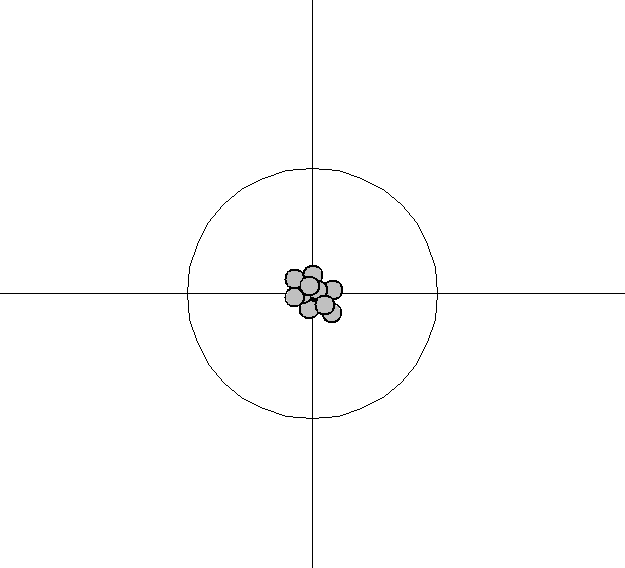
\includegraphics[width=\linewidth]{figures/low-bias-low-variance}
					\caption{Low Bias, Low Variance}
				\end{subfigure}
				~
				\begin{subfigure}{0.3\linewidth}
					\centering
					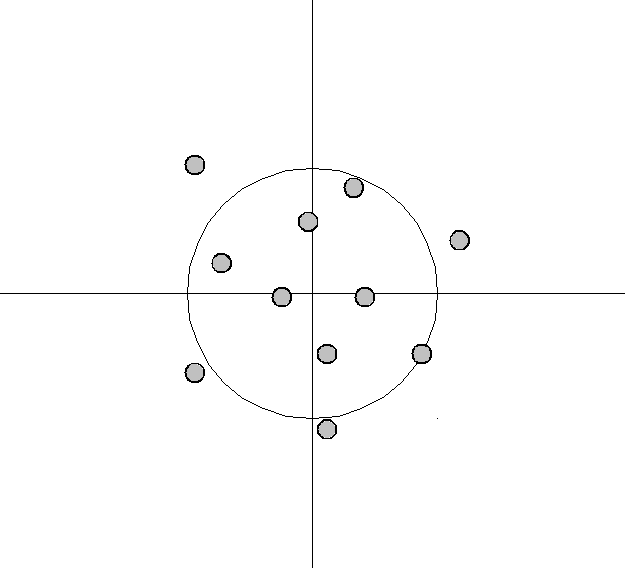
\includegraphics[width=\linewidth]{figures/low-bias-high-variance}
					\caption{Low Bias, High Variance}
				\end{subfigure}
				\\[5pt]
				\begin{subfigure}{0.3\linewidth}
					\centering
					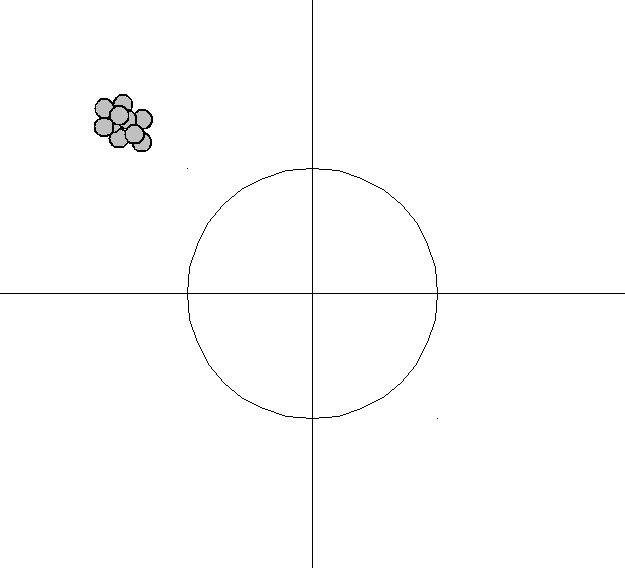
\includegraphics[width=\linewidth]{figures/high-bias-low-variance}
					\caption{High Bias, Low Variance}
				\end{subfigure}
				~
				\begin{subfigure}{0.3\linewidth}
					\centering
					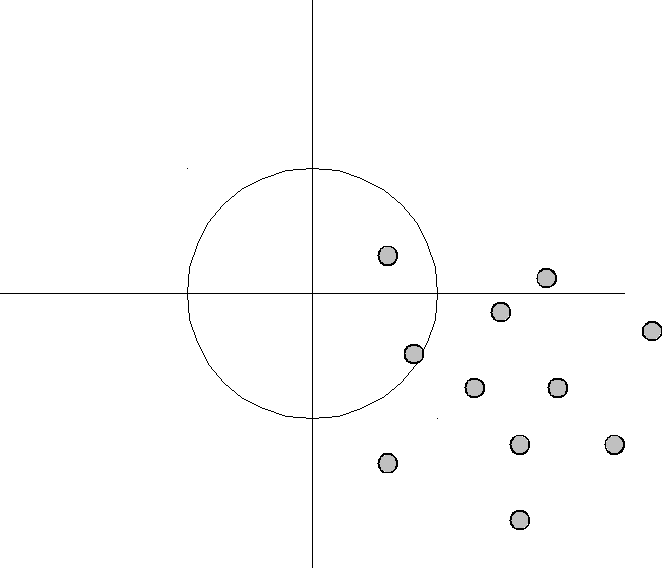
\includegraphics[width=\linewidth]{figures/high-bias-high-variance}
					\caption{High Bias, High Variance}
				\end{subfigure}
				\caption[Bias-Variance Trade-Off]{Bias-Variance Trade-Off; Source: Bernhard Thiery (CC BY-SA 3.0)}
				\label{fig:biasVariance}
			\end{figure}
		% end

		\subsection{Important Sampling}
			\label{subsec:importanceSampling}

			If we want to estimate the expectation of some function \(f(x)\) for \( x \sim p(x) \), but cannot sample from \(p(x)\) (which is often the case for complicated models), we can instead use the following relation(s):
			\begin{gather}
				\E_{x \sim p}\bigl[ f(x) \bigr]
					= \sum_x f(x) p(x)
					= \sum_x f(x) \frac{p(x)}{q(x)} q(x)
					= \E_{x \sim q} \biggl[ f(x) \frac{p(x)}{q(x)} \biggr] \\
				\E_{x \sim p}\bigl[ f(x) \bigr]
					= \int\! f(x) p(x) \dd{x}
					= \int\! f(x) \frac{p(x)}{q(x)} p(x) \dd{x}
					= \E_{x \sim q} \biggl[ f(x) \frac{p(x)}{q(x)} \biggr]
			\end{gather}
			and sample from a surrogate distribution \(q(x)\). This approach obviously has problems if \(q\) does not cover \(p\) sufficiently well along with other problems. See Bishop, 2006, Chapter 11 for details.
		% end

		\subsection{Linear Function Approximation}
			A basic approximator we will need often is the linear function approximator \( f(\vec{x}) = \vec{w}^\transposed \vec{\phi}(\vec{x}) \) with weights \(\vec{w}\) and features \(\vec{\phi}(\vec{x})\). As the weights are optimized and the features are designed, we have lots of variability here. Actually, constructing useful features is the influential step on the approximation quality. Most importantly, features are the only point where we can introduce interactions between different dimensions. A good representations therefore captures all dimensions and all (possibly complex) interaction.

			We will now go over some frequently used features.

			\paragraph{Polynomial Features}
				\emph{Polynomial features} are particularly simple and capture the interaction between dimensions by multiplication. For instance, the first- and second-order polynomial features of a two-dimensional state \( \vec{x} = (x_1, x_2)^\transposed \) are:
				\begin{align}
					\vec{\phi}_\mathit{P1}(\vec{x}) &= (1, x_1, x_2, x_1 x_2)^\transposed &
					\vec{\phi}_\mathit{P2}(\vec{x}) &= (1, x_1, x_2, x_1 x_2, x_1^2, x_2^2, x_1 x_2^2, x_1^2 x_2, x_1^2, x_2^2)
				\end{align}
				However, the number of features grows \emph{exponentially} with the dimension!
			% end

			\paragraph{Fourier Basis}
				Fourier series can be used to approximate periodic functions by adding sine and cosine waves with different frequencies and amplitudes. Similarly, we can use them for general function approximation of functions with bounded domain. As it is possible to approximate any even function with just cosine waves and we are only interested in bounded domains, we can set this domain to positive numbers only and can therefore approximate any function. For one dimension, the \(n\)-th order \emph{Fourier (cosine) basis} is
				\begin{equation}
					\phi_m(x) = \cos(\pi m \tilde{x}),\quad m = 0, 1, \dots, n.
				\end{equation}
				and \( \tilde{x} \) is a normalized version of \(x\), i.e., \( \tilde{x} = (x - x_\mathrm{max}) / (x_\mathrm{max} - x_\mathrm{min}) \).
			% end

			\paragraph{Coarse Coding}
				\emph{Coarse coding} divides the space into \(M\) different regions and produced \(M\)-dimensional coding features for which the \(j\)-th entry is \num{1} iff the data point lies withing the respective region; all values the data point does not lie in are \num{0}. Features with this codomain are also called \emph{sparse.}
			% end

			\paragraph{Tile Coding}
				\emph{Tile coding} is a computationally efficient form of coarse coding which use square \emph{tilings} of space. It uses \(N\) tilings, each composed of \(M\) tiles. The features "vector" is then an \(N \times M\) matrix where a single value is \num{1} iff \(x\) lies inside the tile and \num{0} otherwise. \autoref{fig:tileCoding} shows an illustration of this coding.

				\begin{figure}
					\centering
					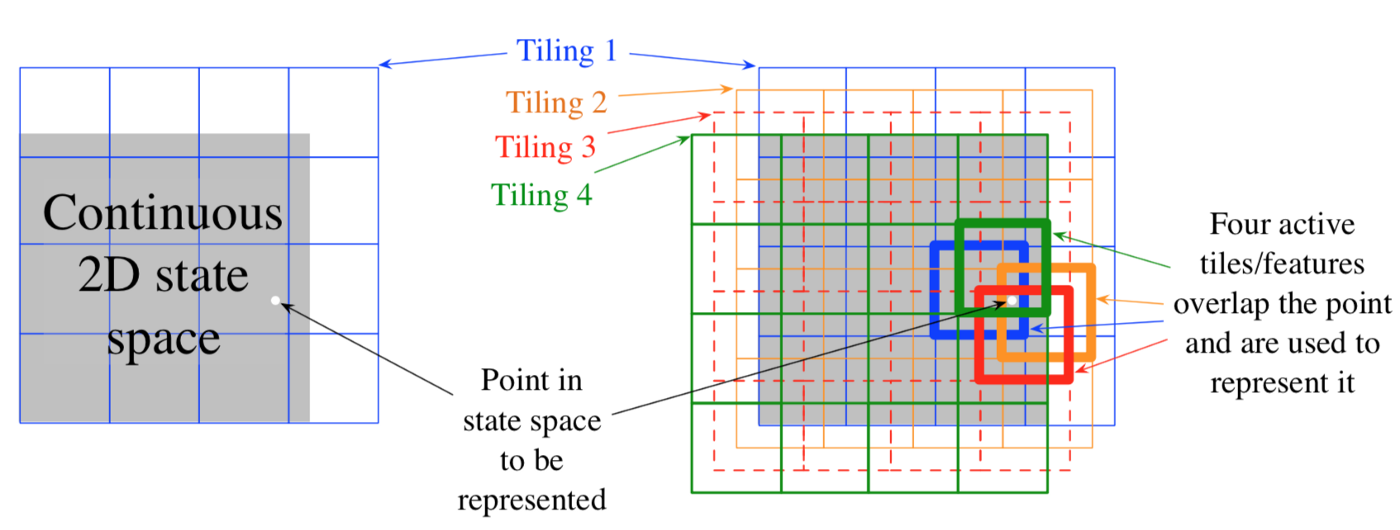
\includegraphics[width=0.9\linewidth]{figures/tile-coding}
					\caption[Tile Coding]{Tile Coding; Source: {\small \url{https://towardsdatascience.com/reinforcement-learning-tile-coding-implementation-7974b600762b}}}
					\label{fig:tileCoding}
				\end{figure}
			% end

			\paragraph{Radial Basis Functions}
				\emph{Radial basis functions (\acsp{RBF}\acused{RBF})} are a generalization of coarse coding where the features are in the interval \((0, 1]\). A typical \ac{RBF} is the Gaussian
				\begin{equation}
					\phi_j(\vec{x}) = \exp\Biggl\{ -\frac{\lVert \vec{x} - \vec{c}_j \rVert_2^2}{2 \sigma_j^2} \Biggr\}
				\end{equation}
				with center \(\vec{c}_j\) and bandwidth \( \sigma_j^2 \).
			% end

			\paragraph{Neural Networks}
				A very powerful alternative to hand-crafting features are \emph{\aclp{NN} (\acsp{NN}\acused{NN}).} By stacking multiple layers of learned features, they are very powerful prediction machines.
			% end
		% end

		\subsection{Likelihood-Ratio Trick}
			\label{subsec:likelihoodRatio}

			Suppose we need to differentiate the expectation of some function \( f(x) \) w.r.t. \(\theta\) where \( x \sim p_\theta(\cdot) \). However, we cannot directly calculate \( \E_{x \sim p_\theta}[f(x)] \) or "differentiate through sampling." Instead, we can use the identity
			\begin{equation}
				\dv{z} \log h(z) = \frac{h'(z)}{h(z)}
				\qquad\implies\qquad
				f'(z) = h(z) \, \dv{z} \log h(z)
			\end{equation}
			to reformulate the derivative of the expectation as
			\begin{equation}
				\pdv{\theta} \E_{x \sim p_\theta}[f(x)]
					= \int\! f(x) \pdv{\theta} p_\theta(x) \dd{x}
					= \int\! f(x) \biggl( \pdv{\theta} p_\theta(x) \biggr) p_\theta(x) \dd{x}
					= \E_{x \sim p_\theta} \biggl[ f(x) \, \pdv{\theta} p_\theta(x) \biggr].
			\end{equation}
			While this is a very powerful approach, the gradient estimator exhibits high variance!
		% end

		\subsection{Reparametrization Trick}
			Suppose we need to differentiate the expectation of some function \( f(x) \) w.r.t. \(\theta\) where \( x \sim p_\theta(\cdot) \). However, we cannot directly calculate \( \E_{x \sim p_\theta}[f(x)] \) or "differentiate through sampling." Instead, we reformulate the expectation with a function \( x = g_\theta(\varepsilon) \) that separates the random components \(\varepsilon\) from the deterministic ones \(\theta\) such that we can reparameterize the expectation as
			\begin{equation}
				\E_{x \sim p_\theta}[f(x)] = \E_\varepsilon\bigl[ f\bigl( g_\theta(\varepsilon) \bigr) \bigr].
			\end{equation}
			For instance, if \( p_\theta(x) = \mathcal{N}(\mu_\theta, \sigma_\theta^2) \) is a Gaussian, \( g_\theta(\varepsilon) = \mu_\theta + \sigma_\theta \varepsilon \) with \( \varepsilon \sim \mathcal{N}(0, 1) \). We can now simply use the chain rule to take the derivative w.r.t. \(\theta\). Compared to the likelihood-ratio trick, this estimator has less variance!
		% end
	% end

	\section{Miscellaneous}
		Finally, this section contains all the stuff that does not fit into the categories before.

		\subsection{Useful Integrals}
			The following hold for a distribution \( p_\theta(x) \):
			\begin{align}
				\int\! \pdv{\theta} p_\theta(x) \dd{x} &= 0 &
				\int\! \pdv{\theta} \log p_\theta(x) \dd{x} &= \int\! \frac{\pdv{\theta} p_\theta(x)}{p_\theta(x)} \dd{x} = 0
				\label{eq:usefulIntegrals}
			\end{align}
			The first identity can be shown by swapping the integral and derivative and using the normalization condition of probability densities. For the second we use integration by parts with \( f' = \pdv{\theta} p_\theta(x) \), for which \(f = 0\) due to the first integral. Hence, the second follows.
		% end
	% end
% end

\chapter{Markov Decision Processes and Policies}
	In this chapter we will develop the groundwork for all upcoming chapters and define some important mathematical concepts.

	\section{Markov Decision Processes}
		A \emph{\ac{MDP}} describes the environment for \ac{RL} \emph{formally} for the case where we can fully observe the environment, i.e., we directly "see" the state. Also, the current state fully characterized the system and future states are independent from the past \emph{(Markov property).} This mathematical framework allows precision and rigorous reasoning on, for instance, optimal solutions and convergence (note, however, that we will only touch the tip of the iceberg in theoretical analysis and we will be less rigorous than some mathematician may wish). The nice this of \acp{MDP} is there wide applicability: we can frame almost all \ac{RL} problems as \acp{MDP}. Most of the remaining chapter here focuses on fully observable and finite \acp{MDP}, i.e., the number of states and actions is finite. \autoref{tab:markovModels} shows an overview over different Markov models.

		We now went over some mathematical definitions for building up the "Markovian framework."

		\begin{table}
			\centering
			\begin{tabular}{c|cc}
				\toprule
				                  & \multicolumn{2}{c}{\textbf{All states observable?}} \\
				\textbf{Actions?} &           Yes           &            No             \\ \midrule
				       Yes        & Markov Decision Process & Partially Observable MDP  \\
				       No         &      Markov Chain       &    Hidden Markov Model    \\ \bottomrule
			\end{tabular}
			\caption{Types of Markov Models}
			\label{tab:markovModels}
		\end{table}

		\begin{definition}[Markov Property]
			A stochastic process \(X_t\) is \emph{Markovian} or \emph{fulfills the Markov property} if \( P_t(S_{t + 1} = s' \given S_t = s, S_{t - 1} = k_{t - 1}, \dots, S_0 = k_0) = P_t(S_{t + 1} = s' \given S_t = s) \) for all \(t\).
		\end{definition}

		\begin{definition}[Stationary Transition Probabilities]
			If \( P_t(S_{t + 1} = s' \given S_t = s) \) is time invariant, \( p_{ss'} \coloneqq P_t(S_{t + 1} = s' \given S_t = s) \) are the \emph{stationary transition probabilities.}
		\end{definition}

		\begin{definition}[State Transition Matrix]
			With the transition probabilities \(p_{ss'}\), let \( \mat{P}_{ss'} \coloneqq p_{ss'} \) for all \(s\), \(s'\) be the \emph{transition matrix.}
		\end{definition}

		\begin{definition}[Markov Chain]
			A \emph{Markov chain} is a tuple \( \langle \mathcal{S}, \mat{P}, \iota \rangle \) with the (finite) set of discrete-time states \(S_t \in \mathcal{S}\), \( n \coloneqq \lvert \mathcal{S} \rvert \), transition matrix \( \mat{P} \in [0, 1]^{n \times n} \), and the initial state distribution \( \iota_i = P(S_0 = i) \).
		\end{definition}

		\begin{definition}[Probability Row Vector]  \label{def:probRowVector}
			The vector \( \vec{p}_t \coloneqq \sum_{i = 1}^{n} P(S_t = i) \vec{e}_i^\transposed \) with the \(i\)-th unit vector \(\vec{e}_i\) and includes the probability of being in the \(i\)-th state at time step \(t\).
		\end{definition}

		\begin{theorem}[Chapman-Kolmogorov for Finite Markov Chains]
			The probability row vector \( \vec{p}_{t + k} \) at time step \(t + k\) starting from \(\vec{p}_t\) at time step \(t\) is given by \( \vec{p}_{t + k} = \vec{p}_t \mat{P}^k \).
		\end{theorem}
		\begin{proof}
			Assume w.l.o.g. \( t = 0 \) We proof this by induction. For the base case, let \(k = 1\). Let \( \vec{p}_0 = (p_{0, 1}, p_{0, 2}, \dots, p_{0, n}) \) be an arbitrary probability row vector. By linearity, we have
			\begin{align}
				\vec{p}_0 \mat{P}_{ss'}
					&= \sum_{i = 1}^{n} p_{0, 1} \vec{e}_i^\transposed \mat{P}
					 = \sum_{i = 1}^{n} p_{0, 1} \mat{P}_i \\
				\intertext{where \(\mat{P}_i\) is the \(i\)-th row of \(\mat{P}\). Rewriting this equation in terms of explicit transition probabilities, we have}
					&= \sum_{i = 1}^{n} P(S_0 = i) \sum_{j = 1}^{n} \vec{e}_j^\transposed P(S_1 = j \given S_0 = i)
					 = \sum_{j = 1}^{n} \vec{e}_j^\transposed \,\sum_{i = 1}^{n} P(S_0 = i) P(S_1 = j \given S_0 = i) \\
					&= \sum_{j = 1}^{n} \vec{e}_j^\transposed \,\sum_{i = 1}^{n} P(S_1 = j, S_0 = i)
					 = \sum_{j = 1}^{n} \vec{e}_j^\transposed P(S_1 = j)
					 = \sum_{j = 1}^{n} p_{1, j} \vec{e}_j^\transposed
					 = \vec{p}_1.
			\end{align}
			The first equality is due to the definition of \(\mat{P}_i\), the third is due to the definition of conditional probabilities, the fourth is due to marginalizing out \(S_0\), and the final is just another application of the definit ion of the probability row vector. For the induction step \( k \to k + 1 \), assume that \( \vec{p}_k = \vec{p}_t \mat{P}^k \) holds for some \(k\). We then have \( \vec{p}_{k + 1} = \vec{p}_k \mat{P} = \vec{p}_0 \mat{P}^k \mat{P} = \vec{p}_0 \mat{P}^{k + 1} \) where the first equality is due to the base case and the second is due to the induction hypothesis.
		\end{proof}

		\begin{definition}[Steady State]
			A probability row vector \(\vec{p}\) is called a \emph{steady} state if an application of the transition matrix does not change it, i.e., \( \vec{p} = \vec{p} \mat{P} \).
		\end{definition}
		\begin{remark}
			While the steady state is in general not independent of the initial state (consider, for instance, \( \mat{P} = \mat{I} \)), it gives insights in which states of the Markov chain are visited in the long run.
		\end{remark}

		\begin{definition}[Absorbing, Ergodic, and Regular Markov Processes]
			A Markov process is called \dots
			\begin{itemize}
				\item \dots \emph{absorbing} if it has at least one \emph{absorbing state} (i.e., a state that can never be left) and if that state can be reached from every other state (not necessarily in one step).
				\item \dots \emph{ergodic} if all states are \emph{recurrent} (i.e., visited an infinite number of times) and \emph{aperiodic} (i.e., visited without a systematic period).
				\item \dots \emph{regular} if some power of the transition matrix has only positive (non-zero) elements.
			\end{itemize}
		\end{definition}

		\subsection{Example}
			\todo{Example; 2.11, 2.12, 2.13}
		% end
	% end

	\section{Markov Reward Processes}
		\begin{definition}{Markov Reward Process}  \label{def:mrp}
			A \emph{Markov reward process} is a tuple \( \langle \mathcal{S}, \mat{P}, R, \gamma, \iota \rangle \) with the (finite) set of discrete-time states \(S_t \in \mathcal{S}\), \(n \coloneqq \lvert \mathcal{S} \rvert\), transition matrix \( \mat{P}_{ss'} = P(s' \given s) \), reward function \( R : \mathcal{S} \to \R : s \mapsto R(s) \), discount factor \( \gamma \in [0, 1] \), and the initial state distribution \( \iota_i = P(S_0 = i) \). We call \( r_t = R(s_t) \) the immediate reward at time step \(t\).
		\end{definition}

		\subsection{Time Horizon, Return, and Discount}
			Note that in \autoref{def:mrp} we did not clearly specify how the reward is computed. Especially we did not define how much time steps the reward "looks" into the future. For this we generally have three options: finite, indefinite, and infinite. The first computes the reward for a fixed and finite number of steps, the second until some stopping criteria is met, and the third infinitely.

			\begin{definition}[Cumulative Reward]
				The \emph{cumulative reward} summarizes the reward signals of a \ac{MRP}. We define the following:
				\begin{align}
					J_t^\mathrm{total} &\coloneqq \sum_{k = 1}^{T} r_{t + k} &
					J_t^\mathrm{average} &\coloneqq \frac{1}{T} \sum_{k = 1}^{T} r_{t + k} &
					J_t \equiv J_t^\mathrm{discounted} &\coloneqq \sum_{k = t + 1}^{T} \gamma^{k - t - 1} r_k,
				\end{align}
				For an infinite horizon, we take the limit of these as \(T \to \infty\).
			\end{definition}
			\begin{theorem}
				The cumulative discounted reward fulfills the recursive relation \( J_t = r_{t + 1} + \gamma J_{t + 1} \).
			\end{theorem}
			\begin{proof}
				\(
					J_t = \sum_{k = t + 1}^{T} \gamma^{k - t - 1} r_k
						= r_{t + 1} + \sum_{k = t + 2}^{T} \gamma^{k - t - 1} r_k
						= r_{t + 1} + \gamma \sum_{k = t + 2}^{T} \gamma^{k - t - 2} r_k
						= r_{t + 1} + \gamma J_{t + 1}
				\)
			\end{proof}
			\begin{definition}[Return]
				The \emph{return} \(J(\tau)\) of a trajectory \( \tau = (s_t)_{t = 1}^{T} \) is the discounted reward \( J(\tau) \coloneqq J_0(\tau) \).
			\end{definition}
			\begin{remark}
				The infinite horizon discounted cumulative reward for \(r_t = 1\) (for all \(t\)) is a geometric series and we have \( J_t = \lim_{T \to \infty} \sum_{k = t + 1}^{T} \gamma^{k - t - 1} r_k = \sum_{k = 0}^{\infty} \gamma^k = 1/(1 - \gamma) \) for \(\gamma < 1\). If the reward is lower/upper bounded by \(r_\mathrm{min}\)/\(r_\mathrm{max}\), we have \( J_t \in \bigl[ r_\mathrm{min}/(1 - \gamma), r_\mathrm{max}/(1 - \gamma) \bigr] \). Similarly, the return is lower/upper-bounded.
			\end{remark}

			We can interpret the discount factor \(\gamma\) as a "measure" how important future rewards are to the current state (how delayed vs. immediate the reward is). For instance, \(\gamma \approx 0\) yields myopic evaluation and \(\gamma \approx 1\) yields far-sighted evaluation. An alternative interpretation is that the discount factor is the probability that the process continues (such that the discounted return is the expected return w.r.t. the discount factor). Despite the obvious advantage that including a discount factor prevents the return from diverging, we also have a couple of other reasons why it makes sense to weigh future rewards less:
			\begin{itemize}
				\item we might be \emph{uncertain} about the future (e.g., with imperfect) models
				\item if the reward is \emph{financial,} immediate rewards earn more interest than delayed rewards
				\item \emph{animal and human behavior} also shows preference for immediate rewards---and why try to mimic biology in the end
			\end{itemize}
			However, sometimes we still use \emph{undiscounted} \acp{MRP} (i.e., \( \gamma = 1 \)), for instance if all sequences are guaranteed to terminate.
		% end

		\subsection{Value Function}
			\begin{definition}[Value Function for MRP]
				The \emph{state value function} for a \ac{MRP} is \( V(s) \coloneqq \E_{\mat{P}}[J_t \given s_t = s] \) for any \(t\).That is, the \emph{expected} return starting from state \(s\) where the expectation is w.r.t. the state dynamics.
			\end{definition}
			\begin{theorem}[Bellman Equation]
				For all states \(s \in \mathcal{S}\), we have \( V(s) = R(s) + \gamma \E\bigl[ V(s_{t + 1}) \biggiven s_t = s \bigr] \).
			\end{theorem}
			\begin{proof}
				\(
					V(s)
						= \E\bigl[ J_t \biggiven s_t = s \bigr]
						= R(s) + \gamma \E\bigl[ J_{t + 1} \biggiven s_t = s \bigr]
						= R(s) + \gamma \E\bigl[ V(s_{t + 1}) \biggiven s_t = s \bigr]
				\)
			\end{proof}
			The Bellman equation allows us to decompose the value of any state into its immediate reward and the value of the subsequent states (in expectation). As we only consider discrete \acp{MRP}, we can also express the Bellman equation in matrix form,
			\begin{equation}
				\vec{V} = \vec{R} + \gamma \mat{P} \vec{V}
				\qquad\iff\qquad
				\vec{V} = (\mat{I} - \gamma \mat{P})^{-1} \vec{R},
				\label{eq:closedFormBellman}
			\end{equation}
			where \(\vec{V}\) and \(\vec{R}\) are columns vectors with the values and rewards, respectively, and \(\mat{P}\) is the transition matrix. We can therefore directly solve this linear equation and get the values of the states! However, for \(n\) states the complexity is \(\mathcal{O}(n^3)\) and hence this is only possible for small \acp{MRP}. For large \acp{MRP}, a variety of efficient iterative methods exist. In the following chapters, we will cover \emph{dynamic programming} (\autoref{c:dp}) \emph{Monte-Carlo evaluation} (\autoref{c:mc}) and \emph{temporal difference learning} (\autoref{c:td}).
		% end

		\subsection{Example}
			\todo{Example; 2.17, 2.22, 2.23, 2.24, 2.26}
		% end
	% end

	\section{Markov Decision Processes}
		So far, we only considered processes \emph{without} actions, i.e., we were not able to interact with the process. The next natural extension is from \acp{MRP} to \acp{MDP}:
		\begin{definition}[Markov Decision Process]
			A \emph{Markov decision process} is a tuple \( \langle \mathcal{S}, \mathcal{A}, \mat{P}, R, \gamma, \iota \rangle \) with the (finite) set of discrete-time states \(S_t \in \mathcal{S}\), \(n \coloneqq \lvert \mathcal{S} \rvert\), (finite) set of actions \(A_t \in \mathcal{A}\), \( m \coloneqq \lvert \mathcal{A} \rvert \), transition matrix \( \mat{P}_{ss'}^{a} = P(s' \given s, a) \), reward function \( R : \mathcal{S} \times \mathcal{A} : (s, a) \mapsto R(s, a) \), discount factor \( \gamma \in [0, 1] \), and the initial state distribution \( \iota_i = P(S_0 = i) \). We call \( r_t = R(s_t) \) the immediate reward at time step \(t\).
		\end{definition}
		An interesting---yet philosophical---question is, whether a scalar reward is adequate to formulate a goal? The big hypothesis underlying its usage is the \emph{Sutton hypothesis} that wall we mean by goals can be formulated as the maximization of a sum of immediate rewards. While this hypothesis might be wrong, it turns out to be so simple and flexible that we just use it. Also, it forces us to simplify our goal and to actually formulate \emph{what} we want instead of \emph{why.} Hence, the goal must be outside of the agent's direct control, i.e., it must not be a component of the agent. However, the agent must be able to measure successes explicitly and frequently.

		In order to reason about an agent and what it might do, we first have to introduce \emph{policies.}

		\subsection{Policies}
			A \emph{policy} defines, at any point in time, what action an agent takes, i.e., it fully defines the \emph{behavior} if the agent. Policies are very flexible and can be Markovian or history-dependent, deterministic or stochastic, stationary or non-stationary, etc.
			\begin{definition}[Policy]
				A \emph{policy} \(\pi\) is a distribution over actions given the state \(s\), i.e., \( \pi(a \given s) = P(a \given s) \).
			\end{definition}
			Note that we can reduce a deterministic policy \( a = \pi(s) \) to a stochastic one using \( \pi(a \given s) = \mathbbm{1}\!\bigl[ a = \pi(s) \bigr] \) for discrete and \( \pi(a \given s) = \delta\bigl( a - \pi(s) \bigr) \) for continuous action spaces. Given an \ac{MDP} \( \mathcal{M} = \langle \mathcal{S}, \mathcal{A}, \mat{P}, R, \gamma, \iota \rangle \) and a policy \(\pi\), let \( \mathcal{M}^\pi = \langle \mathcal{S}, \mathcal{A}, \mat{P}^\pi, R^\pi, \gamma, \iota \rangle \) be the policy \(\pi\)'s \ac{MRP} with
			\begin{align}
				\mat{P}_{ss'}^\pi &= \E_{a \sim \pi(\cdot \given s)}\bigl[ \mat{P}_{ss'}^a \bigr] &
				R^\pi(s) &= \E_{a \sim \pi(\cdot \given s)}\bigl[ R(s, a) \bigr].
				\label{eq:mdpToMrp}
			\end{align}
			This allows us to apply theory of \acp{MRP} and Markov chains to \acp{MDP}. However, it is often useful to exploit the action distribution instead of reducing it to the state dynamics.

			\subsubsection{Value Functions}
				Like for \acp{MRP}, we define the value function for \acp{MDP}:
				\begin{definition}[Value Function for MDP]
					The \emph{state value function} of a \ac{MDP} is \( V^\pi(s) \coloneqq \E_{\mat{P}, \pi}[J_t \given s_t = s] \) for any \(t\). That is, the \emph{expected} return starting from state \(s\) where the expectation is w.r.t. the state dynamics and policy.
				\end{definition}
				However, as we seek to maximize the return and therefore want to steer towards the largest point of the value function, it is helpful to also define the \emph{action} value function:
				\begin{definition}[Action Value Function]
					The \emph{action value function} of a \ac{MDP} is \( Q^\pi(s, a) \coloneqq \E_{\mat{P}, \pi}[J_t \given s_t = s, a_t = a] \) for any \(t\). That is, the \emph{expected} return starting from state \(s\), taking action \(a\) in the first step and subsequently following policy \(\pi\) where the expectation is w.r.t. the state dynamics and policy.
				\end{definition}
				Hence, if we know the action value function for some policy \(\pi\), we can easily choose the action that steers the system to the largest return achievable following \(\pi\) by locally maximizing \(Q(s, a)\) over \(a\) for a given state \(s\): \( \pi(s) = \argmax_a Q(s, a) \).

				Similar to \acp{MRP}, we can also decompose the state and action value function according to a Bellman equation.

				\begin{theorem}[Bellman Expectation Equation]
					For all states \(s \in \mathcal{S}\), we have the following decompositions:
					\begin{align}
						V^\pi(s) &= \E_{a, s'}\bigl[ R(s, a) + \gamma V^\pi(s') \biggiven s \bigr] = \E_{a}\bigl[ Q^\pi(s, a) \bigr] \\
						Q^\pi(s, a) &= R(s, a) + \gamma \E_{s', a'} \bigl[ Q^\pi(s', a') \biggiven s, a \bigr] = R(s, a) + \gamma \E_{s'}\bigl[ V^\pi(s') \biggiven s, a \bigr]  \label{eq:bellmanExpEqQ}
					\end{align}
					Note that the \(Q\)-function decomposition is very similar to the \ac{MRP}-decomposition of the state value function.
				\end{theorem}
				\begin{proof}
					Left as an exercise for the reader (hint: plug in the definitions of the individual components).
				\end{proof}

				Due to the reformulation \eqref{eq:mdpToMrp}, we can reformulate the Bellman equation analogous to \eqref{eq:closedFormBellman} as \( \vec{V}^\pi = \vec{R}^\pi + \gamma \mat{P}^\pi \vec{V}^\pi \) which we can solve in closed form. However, also analogous to the \ac{MRP}-case, this is inefficient for high-dimensional state spaces.

				\begin{definition}[Bellman Operator]  \label{def:bellmanOperator}
					The \emph{Bellman operator} for \(V\) and \(Q\) is an operator \(T^\pi\) mapping from state and action value functions to state and action value functions. It is defined as follows:
					\begin{align}
						(T^\pi V)(s) &= \E_{a, s'}\bigl[ R(s, a) + \gamma V(s') \biggiven s \bigr] \\
						(T^\pi Q)(s, a) &= R(s, a) + \gamma \E_{s', a'} \bigl[ Q(s', a') \biggiven s, a \bigr]
					\end{align}
				\end{definition}
				\begin{theorem}  \label{th:bellmanOperatorContract}
					The Bellman operator is an \(\alpha\)-contraction mapping w.r.t. \( \lVert \cdot \rVert_\infty \) if \( \gamma \in (0, 1) \).
				\end{theorem}
				\begin{proof}
					\todo{Proof: Bellman Contraction}
				\end{proof}
				\begin{remark}
					With these operators, we can compactly write the Bellman equation(s) as \( T^\pi V^\pi = V^\pi \) and \( T^\pi Q^\pi = Q^\pi \) and the policy's state and action value functions are the \emph{unique} respective fixed points of \(T^\pi\). With \autoref{th:bellmanOperatorContract}, repeated application of \(T^\pi\) to any vector converges towards this fixed point.
				\end{remark}
			% end

			\subsubsection{Optimality}
				\begin{definition}[Optimality]  \label{def:optimalValueFunc}
					The optimal state/action-value function is the maximum value over all policies:
					\begin{align}
						V^\ast(s) &\coloneqq \max_\pi V^\pi(s) &
						Q^\ast(s, a) &\coloneqq \max_\pi Q^\pi(s, a).
					\end{align}
					The optimal value function then specifies the \emph{best} possible performance in the \ac{MDP} and we call an \ac{MDP} \emph{solved} when we know the optimal value function.
				\end{definition}
				\begin{definition}[Policy Ordering]
					For two policies \(\pi\), \(\pi'\), we write \( \pi \geq \pi' \) iff \( V^\pi(s) \geq V^{\pi'}(s) \) for all \( s \in \mathcal{S} \).
				\end{definition}
				\begin{theorem}
					For any \acl{MDP} there exists a optimal policy \(\pi^\ast\) with \( \forall \pi : \pi^\ast \geq \pi \) and all policies achieve the unique optimal state- and action-value functions (\autoref{def:optimalValueFunc}). There exists a deterministic optimal policy.
				\end{theorem}
				\begin{remark}
					We can recover the optimal deterministic policy by maximizing \(Q^\ast(s, a)\) over \(a\):
					\begin{equation}
						\pi^\ast(s \given a) =
							\begin{cases*}
								1 & if \( a = \argmax_{a \in \mathcal{A}} Q^\ast(s, a) \) \\
								0 & otherwise
							\end{cases*}
					\end{equation}
				\end{remark}

				With these definitions at hand, we can take a look at Bellman's principle of optimality:
				\begin{center}
					"An optimal policy has the property that whatever the initial state and initial decision are, the remaining decisions must constitute an optimal policy with regard to the state resulting from the first decision." (Richard~Bellman,~1957)
				\end{center}
				This principle is formalized in the \emph{Bellman optimality equation.}

				\begin{theorem}[Bellman Optimality Equation]
					For all states \(s \in \mathcal{S}\), we have the following decompositions:
					\begin{align}
						V^\ast(s) &= \max_{a \in \mathcal{A}} Q^\ast(s, a)
						           = \max_{a \in \mathcal{A}} \;\Bigl\{ R(s, a) + \gamma \E_{s'}\bigl[ V^\ast(s') \biggiven s \bigr] \Bigr\} \\
						Q^\ast(s, a) &= R(s, a) + \gamma \E_{s'}\bigl[ V^\ast(s') \biggiven s \bigr]
						              = R(s, a) + \gamma \E_{s'}\bigl[ \textstyle\max_{a' \in \mathcal{A}}\displaystyle Q^\ast(s', a') \biggiven s \bigr]  \label{eq:bellmanOptEqQ}
					\end{align}
				\end{theorem}
				\begin{proof}
					Left as an exercise for the reader (hint: plug in the definitions of the individual components).
				\end{proof}

				\begin{definition}[Bellman Optimality Operator]  \label{def:bellmanOptimalityOperator}
					The \emph{Bellman optimality operator} for \(V\) and \(Q\) is an operator \(T^\ast\) mapping from state- and action-value functions to state- and action-value functions. It is defined as follows:
					\begin{align}
						(T^\ast V)(s) &= \max_{a \in \mathcal{A}} \;\Bigl\{ R(s, a) + \gamma \E_{s'}\bigl[ V(s') \biggiven s \bigr] \Bigr\} \\
						(T^\ast Q)(s, a) &= R(s, a) + \gamma \E_{s'}\bigl[ \textstyle\max_{a' \in \mathcal{A}}\displaystyle Q(s', a') \biggiven s \bigr]
					\end{align}
				\end{definition}
				\begin{theorem}  \label{th:bellmanOptimalityOperatorContract}
					The Bellman optimality operator is an \(\alpha\)-contraction mapping w.r.t. \( \lVert \cdot \rVert_\infty \) if \( \gamma \in (0, 1) \).
				\end{theorem}
				\begin{proof}
					\todo{Proof: Bellman Contraction}
				\end{proof}
				\begin{remark}
					With these operators, we can compactly write the Bellman equation(s) as \( T^\ast V^\ast = V^\ast \) and \( T^\ast Q^\ast = Q^\ast \) and the optimal state- and action-value functions are the \emph{unique} fixed points of \(T^\ast\). Also, repeated application of \(T^\ast\) to any state- or action-value function converges to the optimal state- or action-value function.
				\end{remark}

				While we had closed-form solutions for the \ac{MRP} and policy value functions, it is not possible to solve the Bellman optimality equation in closed form as its a nonlinear equation system (due to the involved maximizations). In the following chapters we will look at a variety of methods for solving this problem iteratively, starting with \emph{dynamic programming.}
			% end
		% end

		\subsection{Example}
			\todo{Example; 2.31, 2.36, 2.43, 2.45, 2.48}
		% end
	% end

	\section{Wrap-Up}
		\begin{itemize}
			\item definition of \aclp{MRP} and \aclp{MDP}
			\item definition of the two value functions and how to compute them
			\item definition of an optimal policy
			\item the Bellman equation
			\item the Bellman expectation and optimality equations
			\item Additional reading material:
				\begin{itemize}
					\item Book: "Introduction to Reinforcement Learning" (Sutton and Barto, 2018), Chapter 3  % TODO: Read
					\item Book: "Markov Decision Processes" (Puterman, 2005), Chapter 2
				\end{itemize}
		\end{itemize}
	% end
% end

\chapter{Dynamic Programming}
	\label{c:dp}

	In this chapter we will look into a very general approach of solving problem, \emph{\ac{DP},} and will apply it to \acp{MDP}. All these methods have in common that we have a perfect model of the world (e.g., a given \ac{MDP}) and we want to find a policy that maximizes the \ac{MDP}'s reward. The general idea is to break the overall problem down into smaller sub-problems which we then solve optimally. By combining optimal sub-solutions, we get an optimal global solution, assuming that \emph{Bellman's principle of optimality} applies and that the decomposition is possible. An additional assumption is that the sub-problems \emph{overlap,} i.e., they may recur many times and we can cache and reuse their solutions.

	Both of these assumptions are fulfilled by \acp{MDP} where the Bellman equation gives recursive decompositions and the value function stores and reuses solutions. For finite-horizon \acp{MDP}, \ac{DP} is straightforward by starting from \(k = T - 1\) and iterating backwards, \(k = T - 1, T, \dots, 0\), reusing the sub-solutions. The value function and policy are then \(k\)-dependent and we get the optimal value function and policy for \(k = 0\) (when the information was able to "flow" through the \ac{MDP}). Compare to brute-force policy search, we get an exponential speedup! As \ac{DP} for finite-horizon problems is straightforward, we will now stick to infinite-horizon problems.

	Note that we have two central problems we can solve in an \ac{MDP}: \emph{prediction} and \emph{control.} In prediction, we just want to predict the \acp{MDP}'s behavior, i.e., measure its value function given a policy. In control, we want to find the optimal value function and policy. As these problems are closely related and we need the former for the latter, we will discuss them jointly.

	\section{Policy Iteration}
		\emph{\ac{PI}} is an algorithm for solving infinite-horizon \acp{MDP} by repeating the following steps:
		\begin{enumerate}
			\item Policy Evaluation: estimate \(V^\pi\)
			\item Policy Improvement: find a \(\pi' \geq \pi\)
		\end{enumerate}
		The following sections describe these steps in detail and also discuss convergence.

		\subsection{Policy Evaluation}
			In \emph{policy evaluation,} we want to compute the value function \(V^\pi\) for a given policy \(\pi\) (i.e., perform prediction). For this we would either directly solve the Bellman expectation equation using \eqref{eq:closedFormBellman}, but this has complexity \(\mathcal{O}(n^3)\). Instead, we start with some approximation \( V_{k = 0} \) of the value function (which can be arbitrarily bad) and repeatedly apply the Bellman operator (\autoref{def:bellmanOperator}) until convergence:
			\begin{equation}
				V^{(k + 1)}(s)
					\gets (T^\pi V^{(k)})(s)
					= \sum_{a \in \mathcal{A}} \pi(s \given a) \Biggl( R(s, a) + \gamma \sum_{s' \in \mathcal{S}} P(s' \given s, a) V^{(k)}(s') \Biggr).
			\end{equation}
			The sequence \(\bigl(V^{(k)}\bigr)_{k = 0}^{\infty}\) converges, by Banach's fixed point theorem and \autoref{th:bellmanOperatorContract}, to the fixed point \(V^\pi\). In matrix form, we can also write this update as \( \vec{V}^{(k + 1)} = \vec{R}^\pi + \gamma \mat{P}^\pi \vec{V}^{(k)} \).

			However, in subsequent steps we need the action-value function \(Q^\pi\). There are generally two options for this: either recover \(Q^\pi\) from \(V^\pi\) using \eqref{eq:bellmanExpEqQ} or directly estimate it by repeatedly applying its Bellman operator. As this is completely analogous, we will skip the explicit equations here.
		% end

		\subsection{Policy Improvement}
			In \emph{policy improvement,} we want to use find a better policy \(\pi' \geq \pi\) using \(Q^\pi\). We do this by acting greedily, i.e., \( \pi'(s) = \argmax_{a \in \mathcal{A}} Q^\pi(s, a) \). With this definition, we have the following inequality:
			\begin{equation}
				Q^\pi\bigl( s, \pi'(s) \bigr)
					= \max_{a \in \mathcal{A}} Q^\pi(s, a)
					\geq Q^\pi\bigl( s, \pi(s) \bigr)
					= V^\pi(s).
			\end{equation}
			\begin{theorem}[Policy Improvement Theorem]  \label{th:policyImprovement}
				Let \(\pi\) and \(\pi'\) be policies with \( Q^\pi\bigl( s, \pi'(s) \bigr) \geq V^\pi(s) \). Then \( \pi' \geq \pi \).
			\end{theorem}
			\begin{proof}
				By repeatedly applying the premise \((\ast)\), the Bellman expectation equation \((\dagger)\), and the definition of the value function \((\ddagger)\), we find the following inequality chain:
				\begin{align}
					V^\pi(s)
						&\overset{\mathclap{(\ast)}}{=} Q^\pi\bigl( s, \pi'(a) \bigr)
						 \overset{\mathclap{(\dagger)}}{=} \E_{\pi', \mat{P}}\bigl[ r_{t + 1} + \gamma V^\pi(s_{t + 1}) \biggiven s_t = s \bigr]
						 \overset{\mathclap{(\ast)}}{=} \E_{\pi', \mat{P}}\bigl[ r_{t + 1} + \gamma Q^\pi\bigl( s_{t + 1}, \pi'(s_{t + 1}) \bigr) \biggiven s_t = s \bigr] \\
						&\overset{\mathclap{(\ast\dagger)}}{=} \E_{\pi', \mat{P}}\bigl[ r_{t + 1} + \gamma r_{t + 2} + \gamma^2 Q^\pi\bigl( s_{t + 2}, \pi'(s_{t + 2}) \bigr) \biggiven s_t = s \bigr]
						 \overset{\mathclap{(\ast\dagger)}}{=} \E_{\pi', \mat{P}}\bigl[ r_{t + 1} + \gamma r_{t + 2} + \dots \biggiven s_t = s \bigr]
						 \overset{\mathclap{(\ddagger)}}{=} V^{\pi'}(s)
				\end{align}
			\end{proof}

			With this theorem of which the premise is fulfilled when acting greedily, we see that the policy is either improved or, if improvement stops and \( V^{\pi'} = V^\pi \), we found the optimal policy through the Bellman optimality equation \( Q^\pi\bigl( s, \pi(s) \bigr) = V^\pi(s) \). Hence, \ac{PI} always converges to the optimal policy \(\pi^\ast\)!
		% end

		\subsection{Remarks}
			As both policy evaluation and improvement converge to a unique fixed point, policy iteration overall converges to the optimal policy! The algorithm is summarized in \autoref{alg:pi}. Note that recovering \(Q^\pi\) from \(V^\pi\) requires a model of the \ac{MDP}. While this is not a problem for policy iteration as the policy evaluation step requires a model anyway, later on we will estimate the value differently and may not have a model. If so, it makes more sense to directly estimate the action-value function.

			\begin{algorithm}  \DontPrintSemicolon
				\KwIn{Markov decision process \( \mathcal{M} = \langle \mathcal{S}, \mathcal{A}, \mat{P}, R, \gamma, \iota \rangle \)}
				\KwOut{optimal \(V^\ast\), \(Q^\ast\), and \(\pi^\ast\)}
				initialize \( \pi \) arbitrarily \;
				\Repeat{until convergence}{
					\tcp{Policy Evaluation}
					\( k \gets 0 \) \;
					initialize \( Q^{(k)} \) arbitrarily \;
					\Repeat{until convergence}{
						\( V^{(k + 1)}(s) \gets \sum_{a \in \mathcal{A}} \pi(s \given a) R(s, a) + \gamma \sum_{s' \in \mathcal{S}} P(s' \given s, a) Q^{(k)}(s', a) \) \;
						\( k \gets k + 1 \) \;
					}
					\tcp{Recover the action-value function.}
					\( Q^{(\infty)}(s, a) \gets R(s, a) + \gamma \sum_{s' \in \mathcal{S}} P(s' \given s, a) V^{(\infty)}(s') \) \;
					\vspace{5pt}
					\tcp{Policy Improvement}
					\(
						\pi(a \given s) \gets
							\begin{cases}
								1 & \text{if }a = \argmax_{a \in \mathcal{A}} Q^{(\infty)}(s, a) \\
								0 & \text{otherwise}
							\end{cases}
					\) \;
				}
				\Return \( V^{(\infty)} \), \( Q^{(\infty)} \), \( \pi \)
				\caption{Policy Iteration}
				\label{alg:pi}
			\end{algorithm}
		% end

		\subsection{Examples}
			\todo{Example; 3.13, 3.14, 3.15; 3.20, 3.10}
		% end
	% end

	\section{Value Iteration}
		\emph{Value iteration (\acsu{VI})} follows a similar idea as \ac{PI}. However, we do not explicitly compute a policy \(\pi\) but instead only find the optimal value function \(V^\ast\) from which we can recover the optimal policy (using \eqref{eq:bellmanOptEqQ} and greedy updates). To find the optimal value function, we repeatedly apply the Bellman optimality operator (\autoref{def:bellmanOptimalityOperator})
		\begin{equation}
			V^{(k + 1)}(s) = \max_{a \in \mathcal{A}} \;\Bigl\{ R(s, a) + \gamma \E_{s'}\bigl[ V^{(k)}(s') \biggiven s \bigr] \Bigr\}.
		\end{equation}
		As this an \(\alpha\)-contraction due to \autoref{th:bellmanOptimalityOperatorContract}, multiple applications converge to the optimal state-value function \(V^\ast\) for an arbitrary initialization \(V^{(0)}\). This procedure is summarized in \autoref{alg:vi}. We also have the following theorem on the accuracy of the value function estimates.

		\begin{theorem}
			Let \( \lVert V \rVert_\infty = \max_{s \in \mathcal{S}} V(s) \) be the maximum-norm of \(V\) and let \(\epsilon > 0\). If the following inequality holds two successive state-value functions \( V_{i + 1} \) and \( V_i \):
			\begin{equation}
				\lVert V_{i + 1} - V_i \rVert_\infty < \epsilon,
			\end{equation}
			then the error w.r.t. the maximum norm of \(V_{i + 1}\) is upper-bounded by
			\begin{equation}
				\lVert V_{i + 1} - V^\ast \rVert_\infty < \frac{2 \epsilon \gamma}{1 - \gamma}
			\end{equation}
			where \(\gamma\) is the discount factor.
		\end{theorem}

		\begin{algorithm}  \DontPrintSemicolon
			\KwIn{Markov decision process \( \mathcal{M} = \langle \mathcal{S}, \mathcal{A}, \mat{P}, R, \gamma, \iota \rangle \)}
			\KwOut{optimal \(V^\ast\) and \(\pi^\ast\)}
			\tcp{Find optimal state-value function.}
			\( k \gets 0 \) \;
			initialize \( V^{(k)} \) arbitrarily \;
			\Repeat{until convergence}{
				\( V^{(k + 1)}(s) = \max_{a \in \mathcal{A}} \;\Bigl\{ R(s, a) + \gamma \sum_{s' \in \mathcal{S}} P(s' \given s, a) V^{(k)}(s') \Bigr\} \) \;
				\( k \gets k + 1 \) \;
			}
			\tcp{Recover optimal policy.}
			\(
				\pi(a \given s) =
					\begin{cases}
						1 & \text{if }a = \argmax_{a \in \mathcal{A}} \;\Bigl\{ R(s, a) + \gamma \sum_{s' \in \mathcal{S}} P(s' \given s, a) V^{(k)}(s') \Bigr\} \\
						0 & \text{otherwise}
					\end{cases}
			\) \;
			\Return \( V^{(\infty)} \), \( \pi \)
			\caption{Value Iteration}
			\label{alg:vi}
		\end{algorithm}
	% end

	\section{Remarks}
		In \ac{VI}, we had to repeatedly apply max-operations which can be costly. In contrast, \ac{PI} does not require these redundant maximizations, but needs to carry around an explicit policy. However, both algorithms are in the same complexity class: for \(m\) actions and \(n\) states, the state-value based methods is in \( \mathcal{O}(m n^2) \) and the action-value based methods (where instead of recovering \(Q^\pi\) from \(V^\pi\) we estimate it directly) is in \( \mathcal{O}(m^2 n^2) \).

		Note that this chapter only considered \emph{synchronous} \ac{DP} which is only applicable to problems with a relatively small\footnote{A few million, but for high-dimensional problems the state space increases exponentially (cure of dimensionality).} state space. \emph{Asynchronous} \ac{DP}, on the other hand, allows high parallelization and can be applied to larger problems.

		\begin{table}
			\centering
			\begin{tabular}{ccc}
				\toprule
				\textbf{Problem} &           \textbf{Core Equation}            & \textbf{Algorithm} \\ \midrule
				   Prediction    &              Bellman Exp. Eq.               & Policy Evaluation  \\
				    Control      & Bellman Exp. Eq., Greedy Policy Improvement &  Policy Iteration  \\
				    Control      &           Bellman Optimality Eq.            &  Value Iteration   \\ \bottomrule
			\end{tabular}
			\caption{Synchronous Dynamic Programming}
			\label{fig:syncDp}
		\end{table}
	% end

	\section{Wrap-Up}
		\begin{itemize}
			\item dynamic programming
			\item computing optimal policies and value functions for environments with known dynamics
			\item Additional reading material:
				\begin{itemize}
					\item Book: "Introduction to Reinforcement Learning" (Sutton and Barto, 2018), Chapter 4
				\end{itemize}
		\end{itemize}
	% end
% end

\chapter{Monte-Carlo Methods}
	\label{c:mc}

	While \ac{DP} requires a model of the world (in terms of a fully specified \ac{MDP}) and can perform planning inside an \ac{MDP}, \ac{MC} methods and algorithm are \emph{model-free.} They are mostly based on \ac{PI} which---when estimating the action-value functions directly---does not require a model of the world during policy improvement. To evaluate the policy, \ac{MC} methods use repeated random sampling and just produce an estimate. However, they still assume finite \acp{MDP}. We can again identify two tasks:
	\begin{itemize}
		\item \emph{Model-Free Prediction:} estimate the value function of an unknown \ac{MDP} given a policy
		\item \emph{Model-Free Control:} find the optimal value function and policy of an unknown \ac{MDP}; achieved by combining policy improvement with \ac{MC} prediction
	\end{itemize}
	The core idea is to use the mean return of multiple episodes as an estimation for the value of a state. Hence, \ac{MC} methods can only be applied to episodic \acp{MDP}, i.e., ones which eventually terminate. Here we have two options:
	\begin{itemize}
		\item \emph{First-Visit \ac{MC}:} estimate the value of a state \(s\) by averaging the returns \emph{only for the first time} \(s\) is visited in an episode; yields an \emph{unbiased} estimator; see \autoref{alg:firstVisitMCPE}
		\item \emph{Every-Visit \ac{MC}:} estimate the value of a state \(s\) by averaging the returns \emph{every time} \(s\) is visited in an episode; yields a \emph{biased} but still \emph{consistent} estimator; see \autoref{alg:everyVisitMCPE}
	\end{itemize}
	\todo{MC: Why is first-visit biased and every-visit only consistent?}

	\begin{algorithm}  \DontPrintSemicolon
		\KwIn{policy \(\pi\)}
		\KwOut{approximate \(V^\pi\)}
		initialize \(V^{(k)}\) arbitrarily \;
		initialize \(\mathit{Returns}(s)\) as an empty list for all \(s \in \mathcal{S}\) \;
		\Repeat{convergence}{
			\( (s_0; r_1, s_1; r_2, s_2; \dots; r_{T - 1}, s_{T - 1}, r_T) \gets \text{generate episode} \) \;
			\ForEach{\( t = 0, 1, \dots, T \)}{
				\If{\(s_t\) is visited for the first time}{
					\( J_t \gets \sum_{k = t + 1}^{T} \gamma^{k - t - 1} r_k \)  \quad\tcp{cumulative discounted reward}
					append \(J_t\) to \(\mathit{Returns}(s_t)\) \;
					\( V(s_t) \gets \text{average}\bigl(\mathit{Returns}(s_t)\bigr) \)  \quad\tcp{update value estimate}
				}
			}
		}
		\Return \(V\) \;
		\caption{First-Visit Monte-Carlo Policy Evaluation}
		\label{alg:firstVisitMCPE}
	\end{algorithm}
	\begin{algorithm}  \DontPrintSemicolon
		\KwIn{policy \(\pi\)}
		\KwOut{approximate \(V^\pi\)}
		initialize \(V^{(k)}\) arbitrarily \;
		initialize \(\mathit{Returns}(s)\) as an empty list for all \(s \in \mathcal{S}\) \;
		\Repeat{convergence}{
			\( (s_0; r_1, s_1; r_2, s_2; \dots; r_{T - 1}, s_{T - 1}, r_T) \gets \text{generate episode} \) \;
			\ForEach{\( t = 0, 1, \dots, T \)}{
				\( J_t \gets \sum_{k = t + 1}^{T} \gamma^{k - t - 1} r_k \)  \quad\tcp{cumulative discounted reward}
				append \(J_t\) to \(\mathit{Returns}(s_t)\) \;
				\( V(s_t) \gets \text{average}\bigl(\mathit{Returns}(s_t)\bigr) \)  \quad\tcp{update value estimate}
			}
		}
		\Return \(V\) \;
		\caption{Every-Visit Monte-Carlo Policy Evaluation}
		\label{alg:everyVisitMCPE}
	\end{algorithm}

	\section{Example}
		\todo{Example; 3.42, 3.43, 3.44, 3.45, 3.46, 3.47, 3.48, 3.49, 3.50, 3.51, 3.52, 3.53, 3.54, 3.55, 3.56, 3.57}
	% end

	\section{Wrap-Up}
		\begin{itemize}
			\item approximation of value functions when the dynamics are not available
			\item differences of \ac{DP} and \ac{MC}
			\item Additional reading material:
				\begin{itemize}
					\item Book: "Introduction to Reinforcement Learning" (Sutton and Barto, 2018), Chapter 5  % TODO: Read
					\item Book: "Monte-Carlo Simulation-Based Statistical Modeling" (Chen and Chen, 2017)
				\end{itemize}
		\end{itemize}
	% end
% end

\chapter{Temporal Difference Learning}
	\label{c:td}

	We will now turn to methods that feel more like "reinforcement learning" rather than \ac{DP} and control theory: \emph{\ac{TD} learning.} Like \ac{MC} methods, \ac{TD} learning learns directly from experience and is also \emph{model-free,} i.e., it has no knowledge of the \ac{MDP} dynamics. However, \ac{TD} methods can learn from incomplete episodes and therefore do not require episodic \acp{MDP}, making them readily applicable to all kinds of problems. The core idea is to update an estimate towards a \emph{better estimate.} Consider \emph{incremental} every-visit \ac{MC} policy evaluation,
	\begin{equation}
		V(s_t) \gets V(s_t) + \alpha \bigl( J_t - V(s_t) \bigr) = (1 - \alpha) V(s_t) + \alpha J_t,  \label{eq:mcUpdate}
	\end{equation}
	where \(J_t\) is the return following \(s_t\) and \(\alpha\) is a trade-off between the two estimates. Note that for \( \alpha = 1/(K + 1) \) where \(K\) is the number of samples collected before this sample, this update reduces to plain every-visit \ac{MC}. The idea of \ac{TD} learning is to replace the return \(J_t\) which requires all future samples with an estimate of the return using the immediate reward \(r_{t + 1}\) together with an estimate of the value function \(V_{t + 1}\). This process of using an estimate to update another estimate is called \emph{bootstrapping.} This yields the simplest \ac{TD} learning algorithm, TD(\(0\)), with the following update:
	\begin{equation}
		V(s_t) \gets V(s_t) + \alpha \bigl( r_{t + 1} + \gamma V(s_{t + 1}) - V(s_t) \bigr) = V(s_t) + \alpha \delta_t.  \label{eq:tdUpdate}
	\end{equation}
	We call \( r_{t + 1} + \gamma V(s_t) \) the \emph{\ac{TD} target} and \( \delta_t \coloneqq r_{t + 1} + \gamma V(s_t) - V(s_t) \) the \emph{\ac{TD} error.} Again, \(\alpha\) is a trade-off between the two estimates where \(\alpha \approx 0\) just sticks to the previous estimate and \(\alpha \approx 1\) directly jumps to the new (bootstrapped) estimate.

	\begin{algorithm}  \DontPrintSemicolon
		\KwIn{environment}
		\KwOut{value function}
		\Repeat{convergence}{
			initialize \(s\) \;
			\While{\(s\) is not terminal}{
				take action \( a \sim \pi(\cdot \given s) \), observe reward \(r\) and next state \(s'\) \;
				\( \delta \gets r + \gamma V(s') - V(s) \) \;
				\( V(s) \gets V(s) + \alpha \delta \) \;
				\( s \gets s' \) \;
			}
		}
		\Return \(V\) \;
		\caption{TD(\(0\))}
		\label{alg:td0}
	\end{algorithm}

	\section{Temporal Differences vs. Monte-Carlo (vs. Dynamic Programming)}
		While both \ac{TD} and \ac{MC} methods are model-free, they still have some major differences. Firstly, \ac{TD} can learn before and even \emph{without} knowing the final outcome of an episode. This enables online learning (i.e., learning while running) whereas \ac{MC} has to wait for an episode to end and the final return is known before learning anything. This directly transfers to continuing (i.e., non-terminating) environments where \ac{TD} can be employed and \ac{MC} cannot.

		As usual, we have a bias-variance trade-off between the methods, or more precisely between the two updates \eqref{eq:mcUpdate} and \eqref{eq:tdUpdate}. While the return \(J_t\) is an unbiased estimate of \(V^\pi(s_t)\) and therefore the (first-visit) \ac{MC} update is unbiased, the \ac{TD} target has much lower variance as it only depends on a single random action-transition-reward triple. However, the \ac{TD} target is biased unless \( V(s_{t + 1}) = V^\pi(s_t) \), i.e., the true value function, is found.

		While \ac{TD} actively exploits the Markov property, \ac{MC} does not at all. Of course, this makes \ac{MC} more well-rounded and applicable to non-Markovian environments while \ac{TD}'s wrong assumptions can hurts its efficiency. However, for very complicated environments we might not be able to use tabular methods (\autoref{c:tabular}), but have to resort to function approximations (\autoref{c:funcApprox}) where \ac{MC} excels. Also, \ac{TD} is more efficient to the initial values as \ac{MC} which makes sense as \ac{MC} might not use them at all.

		See \autoref{fig:comparisonDpMcTd} for a comparison of \ac{DP}, \ac{MC}, and \ac{TD} with regard to bootstrapping and sampling.

		\begin{table}
			\centering
			\begin{tabular}{c|cc}
				\toprule
				  \textbf{Method}    & \textbf{Uses Bootstrapping} & \textbf{Uses Sampling} \\ \midrule
				Dynamic Programming  &             Yes             &           No           \\
				    Monte-Carlo      &             No              &          Yes           \\
				Temporal Differences &             Yes             &          Yes           \\ \bottomrule
			\end{tabular}
			\caption{Dynamic Programming vs. Monte-Carlo vs. Temporal Difference}
			\label{fig:comparisonDpMcTd}
		\end{table}

		\subsection{Backup}
			\todo{TD/MC: Backup; 3.69, 3.70, 3.71}
		% end
	% end

	\section{\acs{TD}(\(\lambda\))}
		\label{sec:tdLambda}

		Looking at \eqref{eq:tdUpdate}, one might ask why we only look \emph{one} step into the future an not, for instance, three steps. In fact, this is possible and we can consider the \emph{\(n\)-step return}
		\begin{equation}
			J_t^{(n)} \coloneqq r_{t + 1} + \gamma r_{t + 2} + \dots + \gamma^{n - 1} r_{t + n} + \gamma^n V(s_{t + n})
		\end{equation}
		with \(n\)-step \ac{TD} learning,
		\begin{equation}
			V(s_t) \gets V(s_t) + \alpha \bigl( J_t^{(n)} - V(s_t) \bigr).
		\end{equation}
		Increasing \(n\) has the advantage of reducing the estimate's bias for the cost of increasing its variance (as with a larger \(n\), more random factors come into play). With \(n \to \infty\), this update approaches \eqref{eq:mcUpdate}, the \ac{MC} update.

		\subsection{Forward-View}
			The natural next idea is to average multiple \(n\)-step returns to combine information from different time steps. For instance, we could average the \(2\)- and \(4\)-step returns \( \tilde{J} = J^{(2)}/2 + J^{(4)}/2 \). But can we come up with a principled way of weighing different \(n\)-step returns? A fruitful idea is to use an exponential weighting, i.e., to weigh samples in the future exponentially less than close samples. This is the idea of the \emph{\(\lambda\)-return}
			\begin{equation}
				J_t^\lambda = (1 - \lambda) \sum_{n = 1}^{\infty} \lambda^{n - 1} J_t^{(n)}
			\end{equation}
			which uses the weighting function \( (1 - \lambda) \lambda^{n - 1} \), \( \lambda \in [0, 1) \) for the \(n\)-step return. The factor \((1 - \lambda)\) is necessary for the sum to be convex, i.e.,
			\begin{equation}
				(1 - \lambda) \sum_{n = 1}^{\infty} \lambda^{n - 1}
					= (1 - \lambda) \sum_{n = 0}^{\infty} \lambda^n
					= (1 - \lambda) \frac{1}{1 - \lambda}
					= 1.
			\end{equation}
			We call the resulting update \( V(s_t) \gets V(s_t) + \alpha \bigl( J_t^\lambda - V(s_t) \bigr) \) \emph{forward-view TD(\(\lambda\)).} Of course now we are back to the initial problem we tried to avoid using \ac{TD} methods: the forward-view \ac{TD} target can only be computed for complete episodes!
		% end

		\subsection{Backward-View and Eligibility Traces}
			We saw that forward-view TD(\(\lambda\)) provides a good approach to reduce the bias of the \ac{TD} target. However, it had the disadvantage of only working in episodic settings, i.e., only with complete episodes. An alternative is \emph{backward-view TD(\(\lambda\))} following a similar idea, but looking backward in time, allowing updates from incomplete episodes. However, now we have the \emph{credit assignment problem:} how to weigh past rewards and states? Two common heuristics are the \emph{frequency} and \emph{recency} heuristic, i.e., assigning credit to the most frequent or most recent states, respectively. Both of these ideas can be summarized into \emph{eligibility traces.} For every time step \(t\), we keep an eligibility value \( z_t(s) \) for every state \(s\) describing the weight of state \(s\) at time step \(t\). Starting with \( z_{-1}(s) = 0 \), we iteratively compute the next time step as
			\begin{equation}
				z_t(s) = \gamma \lambda z_{t - 1}(s) + \mathbbm{1}[s = s_t],
			\end{equation}
			where \(\gamma\) is the discount factor and \(\lambda\) is the exponential decay for the eligibility. The intuition of this update is as follows: Whenever we take a step in the environment, we decrease the weight by multiplying with \(\lambda\) (implementing the recency heuristic); by adding one whenever we see a state, we implement the frequency heuristic (by adding one often for frequent states) and "give the recency heuristic something to work with," i.e., some value it can actually decrease. The update (applied to all states and not just the current state) then is
			\begin{equation}
				V(s) \gets V(s) + \alpha \delta_t z_t(s)
			\end{equation}
			where \(\delta_t\) is the \ac{TD} error. Note that for \(\lambda = 0\), the update collapses exactly on the TD(\(0\)) update \eqref{eq:tdUpdate}, hence the name. The algorithm is summarized in \autoref{alg:backwardViewTdLambda}.

			\todo{Backward-View TD(lambda): Equivalence of forward- and backward-view.}

			\begin{algorithm}  \DontPrintSemicolon
				\KwIn{environment}
				\KwOut{value function}
				\Repeat{converged}{
					\( z(s) \gets 0 \) for all \( s \in \mathcal{S} \) \;
					initialize \(s\) \;
					\While{\(s\) is not terminal}{
						take action \( a \sim \pi(\cdot \given s) \), observe reward \(r\) and next state \(s'\) \;
						\( \delta \gets r + \gamma V(s') - V(s) \) \;
						% TODO: Backward-View TD(lambda): Why update the eligibility traces like this and not like the equation states?
						\( z(s) \gets z(s) + 1 \) \;
						\ForEach{\( \tilde{s} \in \mathcal{S} \)}{
							\( V(\tilde{s}) \gets V(\tilde{s}) + \alpha \delta z(\tilde{s}) \) \;
							\( z(\tilde{s}) \gets \gamma \lambda z(\tilde{s}) \) \;
						}
						\( s \gets s' \) \;
					}
				}
				\Return \(V\) \;
				\caption{Backward-View TD(\(\lambda\))}
				\label{alg:backwardViewTdLambda}
			\end{algorithm}
		% end
	% end

	\section{Example}
		\todo{Example; 3.61, 3.62}
	% end

	\section{Wrap-Up}
		\begin{itemize}
			\item differences of \ac{DP}, \ac{MC}, and \ac{TD}
			\item definition of eligibility traces
			\item computation of TD(\(\lambda\))
			\item Additional reading material:
				\begin{itemize}
					\item Book: "Introduction to Reinforcement Learning" (Sutton and Barto, 2018), Chapters 6, 7, and 12  % TODO: Read
				\end{itemize}
		\end{itemize}
	% end
% end

\chapter{Tabular Reinforcement Learning}
	In this chapter we cover methods from \emph{tabular} \ac{RL} where the state-action-space is small enough such that we can represent the action-value function as a table. We distinguish two categories of methods: on- and off-policy learning. In the former the algorithm learns "on the job," i.e., the experience is sampled from the policy that is being trained. In the latter the algorithms learns "by looking over someone's shoulder," i.e., the experience is samples from a different policy \(q\) that the one that is being trained.

	\section{On-Policy Methods}
		In this section we discuss tabular on-policy methods.

		\subsection{Monte-Carlo Methods and Exploration vs. Exploitation}
			\label{subsec:mcExploration}

			In \emph{generalized} \ac{PI}, we do not evaluate the state-value function (for which a greedy policy improvement needs the transition dynamics), but instead evaluate the action-value. However, just using the deterministic policy found during policy improvement for \ac{MC} policy evaluation means that we do not have exploration (no "new" actions are tried)! This brings us to the \emph{exploration vs. exploitation dilemma.}

			During decision-making, we have two options: \emph{exploit} the current knowledge to make the best known decision or \emph{explore} and gather more information. In other words, the best long-term options (which we want to find) might involve short-term sacrifices. This dilemma is a fundamental problem in \ac{RL} and we do not have a satisfying solution yet. Two common approaches are \emph{\(\epsilon\)-greedy},
			\begin{align}
				a =
					\begin{cases*}
						a^\ast & with probability \(1 - \epsilon\) \\
						\text{random action} & with probability \(\epsilon\)
					\end{cases*},
			\end{align}
			and \emph{softmax.} A softmax policy biases the action selection towards exploitation. The most common softmax is the Boltzmann distribution
			\begin{equation}
				\pi(a \given s) = \frac{\exp\bigl\{ Q(s, a) / \tau \bigr\}}{\exp\bigl\{ \sum_{a' \in \mathcal{A}} Q(s, a') / \tau \bigr\}}
			\end{equation}
			with a \emph{temperature} \(\tau\) defining how uniform the distribution is. For \(\tau \to \infty\), the distribution approaches a uniform distribution of \(a\) and for \(\tau = 0\) it acts greedy.

			\subsubsection{\(\epsilon\)-Greedy Exploration and Policy Improvement}
				The simplest exploration strategy, \(\epsilon\)-greedy, can also be formulated as a distribution:
				\begin{equation}
					\pi(a \given s) =
						\begin{cases*}
							\epsilon/m + 1 - \epsilon & if \( a = \argmax_{a \in \mathcal{A}} Q(s, a) \) \\
							\epsilon/m                & otherwise
						\end{cases*}
				\end{equation}
				Interestingly, the \(\epsilon\)-greedy policy still causes monotonic improvements as for any \(\epsilon\)-greedy policy \(\pi\), the \(\epsilon\)-greedy policy w.r.t. \(Q^\pi\) fulfills the premise of the policy improvement theorem (\autoref{th:policyImprovement}):
				\begin{align}
					Q^\pi\bigl( s, \pi'(s) \bigr)
						&= \sum_{a \in \mathcal{A}} \pi'(a \given s) Q^\pi(s, a)
					 = \sum_{a \in \mathcal{A}} Q^\pi(s, a)
							\begin{cases*}
								\epsilon/m + 1 - \epsilon & if \( a = \argmax_{a \in \mathcal{A}} Q^\pi(s, a) \) \\
								\epsilon/m                & otherwise
							\end{cases*} \\
						&\overset{\mathclap{(\ast)}}{=} \frac{\epsilon}{m} \sum_{a \in \mathcal{A}} Q^\pi(s, a) + (1 - \epsilon) \max_{a \in \mathcal{A}} Q^\pi(s, a) \\
						&\overset{\mathclap{(\dagger)}}{\geq} \frac{\epsilon}{m} \sum_{a \in \mathcal{A}} Q^\pi(s, a) + (1 - \epsilon) \sum_{a \in \mathcal{A}} \frac{\pi(a \given s) - \epsilon/m}{1 - \epsilon} Q^\pi(s, a)
					 \overset{\mathclap{(\ddagger)}}{=} \sum_{a \in \mathcal{A}} \pi(a \given s) Q^\pi(s, a)
					 = V^\pi(s)
				\end{align}
				In step \((\ast)\) we explicitly plugged in the policy \(\pi'\) using that its first case is applied exactly once for the maximum of \(Q^\pi(s, a)\). Hence, we can pull it out of the sum. In step \((\dagger)\), we "inverse plugged in" an \(\epsilon\)-greedy policy using the relations
				\begin{align}
					\frac{\pi(a \given s) - \epsilon/m}{1 - \epsilon} &= \frac{\epsilon/m - \epsilon/m}{1 - \epsilon} = 0 &
					\frac{\pi(a \given s) - \epsilon/m}{1 - \epsilon} &= \frac{\epsilon/m + 1 - \epsilon - \epsilon/m}{1 - \epsilon} = 1
				\end{align}
				for the "maximum" \(a\) and all others, respectively. Note that this maximum is \emph{not} w.r.t. \( Q^\pi(s, a) \) and hence the sum over all actions must be less than or equal to the maximum value of \(Q^\pi(s, a)\). Finally, in step \((\ddagger)\), we used the definition of \(\pi\) and that \(Q^\pi(s, a)\) is its action-value function.

				Using \(\epsilon\)-greedy exploration therefore gives monotonic improvement while not shutting canceling exploration during policy evaluation!
			% end

			\subsubsection{\acs{GLIE} Monte-Carlo}
				\begin{definition}[Greedy in the Limit of Infinite Exploration (\acs{GLIE})]
					A policy \(\pi\) is \emph{\acl{GLIE} (\acsu{GLIE})} if all state-action pairs are explore infinitely many times,
					\begin{equation}
						\lim\limits_{k \to \infty} N^{(k)}(s, a) \to \infty,
					\end{equation}
					and the policy converges to a greedy policy,
					\begin{equation}
						\lim\limits_{k \to \infty} \pi_k(a \given s) = \mathbbm{1}\bigl[ a = \argmax_{a' \in \mathcal{A}} Q^{(k)}(s, a') \bigr].
					\end{equation}
					Here \(k\) is the policy iteration index.
				\end{definition}

				\ac{GLIE} \ac{MC} achieves this by choosing \( \epsilon_k = 1/k \) and \( \pi = \epsilon\text{-greedy} \). We then also have the following theorem.

				\begin{theorem}[Convergence of \acs{GLIE} Monte-Carlo]
					\ac{GLIE} \ac{MC} converges to the \emph{optimal} action-value function.
				\end{theorem}
			% end
		% end

		\subsection{\acs{TD}-Learning: \acs{SARSA}}
			We already saw in \autoref{c:td} that \ac{TD} learning has several advantages over \ac{MC}, namely lower variance, online capabilities, and learning from incomplete sequences. So a natural idea is to replace \ac{MC} with \ac{TD} in the control loop, i.e., applying \ac{TD} to the action-value function using \(\epsilon\)-greedy policy improvement. In \acsu{SARSA} (for "\acl{SARSA}"), we use the policy's proposed action during the \ac{TD} update, i.e.,
			\begin{equation}
				Q(s_t, a_t) \gets Q(s_t, a_t) + \alpha \bigl( r_{t + 1} + \gamma Q(s_{t + 1}, a_{t + 1}) - Q(s_t, a_t) \bigr),
			\end{equation}
			where \( a_{t + 1} \sim \pi^Q(\cdot \given s_{t + 1}) \) is sampled from a policy derived from \(Q\) (indicated by the superscript). Hence, \ac{SARSA} is an on-policy algorithm. The pseudocode is depicted in \autoref{alg:sarsa}. If we choose the step sizes \(\alpha\) wisely, we also have convergence guarantees!

			\begin{theorem}[Convergence of \acs{SARSA}]
				If the policies \( \pi_t(s, a) \) constitute a \ac{GLIE} sequence and the step sizes \(\alpha_t\) constitute a Robbins-Monro sequence, i.e., \( \sum_{t = 1}^{\infty} \alpha_t = \infty \) and \( \sum_{t = 1}^{\infty} \alpha_t^2 < \infty \), \ac{SARSA} converges to the optimal action-value function.
			\end{theorem}

			\begin{algorithm}  \DontPrintSemicolon
				\KwIn{environment}
				\KwOut{(optimal) action-value function}
				initialize \(Q\) arbitrarily except \(Q(\mathrm{terminal}, \cdot) = 0\) \;
				\Repeat{converged}{
					initialize \(s\) \;
					choose \( a \sim \pi^Q(\cdot \given s) \) \;
					\While{\(s\) is not terminal}{
						take action \(a\), observe reward \(r\) and next state \(s'\) \;
						choose \( a' \sim \pi^Q(\cdot \given s') \) \;
						\( \delta \gets r + \gamma Q(s', a') - Q(s, a) \) \;
						\( Q(s, a) \gets Q(s, a) + \alpha \delta \) \;
						\( s \gets s' \) \;
						\( a \gets a' \) \;
					}
				}
				\Return \(Q\) \;
				\caption{\acs{SARSA}}
				\label{alg:sarsa}
			\end{algorithm}

			\subsubsection{Eligibility Traces and \acs{SARSA}(\(\lambda\))}
				Similar to \acs{TD}(\(\lambda\)) (\autoref{sec:tdLambda}), could use the \(n\)-step return \(J_t^{(n)}\) in the \ac{SARSA} update,
				\begin{equation}
					Q(s_t, a_t) \gets Q(s_t, a_t) + \alpha \bigl( J_t^{(n)} - Q(s_t, a_t) \bigr).
				\end{equation}
				We can again generalize this to the \(\lambda\)-return \(J_t^\lambda\) with exponential decay. However, we have the same disadvantage with this \emph{forward-view} as before: now we need complete sequences to calculate the TD target! Hence, we instead use the equivalent \emph{backward-view} and eligibility traces for state-action pairs,
				\begin{equation}
					z_t(s, a) = \gamma \lambda z_{t - 1}(s, a) + \mathbbm{1}[s = s_t, a = a_t],
				\end{equation}
				kicking the recursion off with \( z_{-1}(s, a) = 0 \).

				\begin{algorithm}  \DontPrintSemicolon
					\KwIn{environment}
					\KwOut{(optimal) action-value function}
					initialize \(Q\) arbitrarily except \(Q(\mathrm{terminal}, \cdot) = 0\) \;
					\Repeat{converged}{
						\( z(s, a) \gets 0 \) for all \(s \in \mathcal{S}\) and \(a \in \mathcal{A}\) \;
						initialize \(s\) \;
						choose \( a \sim \pi^Q(\cdot \given s) \) \;
						\While{\(s\) is not terminal}{
							take action \(a\), observe reward \(r\) and next state \(s'\) \;
							choose \( a' \sim \pi^Q(\cdot \given s') \) \;
							\( \delta \gets r + \gamma Q(s', a') - Q(s, a) \) \;
							\( z(s, a) \gets z(s, a) + 1 \) \;
							\ForEach{\( \tilde{s} \in \mathcal{S} \)}{
								\( Q(s, a) \gets Q(s, a) + \alpha \delta z(s, a) \) \;
								\( z(s, a) \gets \gamma \lambda z(s, a) \) \;
							}
							\( s \gets s' \) \;
							\( a \gets a' \) \;
						}
					}
					\Return \(Q\) \;
					\caption{\acs{SARSA}(\(\lambda\))}
					\label{alg:sarsaLambda}
				\end{algorithm}
			% end

			\subsubsection{Example}
				\todo{Example; 4.28, 4.29, 4.33}
			% end
		% end
	% end

	\section{Off-Policy Methods}
		While on-policy methods are great and often exhibit convergence guarantees, they have a major flaw: exploration has to be built into the policy, for instance using \(\epsilon\)-greed. \emph{Off-policy} methods, on the other hand, learn about a target policy \(\pi(a \given s)\) while following a behavioral policy \(q(a \given s)\). We can directly transfer this approach to a variety of tasks such as learning directly from a human or other agents, re-use experience of old policies, explore while learning an optimal policy, or learning multiple policies while following a single.

		\subsection{Monte-Carlo}
			The core concept for off-policy \ac{MC} is \emph{importance sampling} (\autoref{subsec:importanceSampling}). Hence, we update the return \(J_t\) sampled from a behavioral policy \(q\) by the importance sampling corrections,
			\begin{equation}
				J_t^{\pi/q} = \frac{\pi(a_t \given s_t)}{q(a_t \given s_t)} \frac{\pi(a_{t + 1} \given s_{t + 1})}{q(a_t \given s_t)} \cdots \frac{\pi(a_T \given s_T)}{q(a_T \given s_T)} J_t.
			\end{equation}
			Note that we only need to correct using the policy distributions even though the return distribution contains factors of the state dynamics. However, these are the same for both policies so they cancel in the importance sampling weights. We then update the action-value towards this corrected return:
			\begin{equation}
				Q(s_t, a_t) \gets Q(s_t, a_t) + \alpha \bigl( J_t^{\pi/q} - Q(s_t, a_t) \bigr).
			\end{equation}
			While this allows off-policy \ac{MC}, importance sampling can dramatically increase the variance even further! Also, it is not possible to sample actions for which \(q\) is zero but \(\pi\) is non-zero.
		% end

		\subsection{\acs{TD} and Q-Learning}
			Similar to off-policy \ac{MC}, we can also use importance sampling in \ac{TD} learning by weighing the \ac{TD} error accordingly:
			\begin{align}
				\rho_t &= \frac{\pi(a_t \given s_t)}{q(s_t \given a_t)} &
				V(s_t) &\gets V(s_t) + \alpha \rho_t \delta_t.
			\end{align}
			Compared to \ac{MC}, the \ac{TD} has much lower variance and the policies only need to be similar over a single step, hence the risk of \(q \approx 0\) is reduced. But we can do better and mitigate the use of importance sampling at all!

			In \emph{Q-learning,} we update the action-value towards the value of an alternative action,
			\begin{equation}
				Q(s_t, a_t) \gets Q(s_t, a_t) + \alpha \bigl( r_{t + 1} + \gamma Q(s_t, a') - Q(s_t, a_t) \bigr),  \label{eq:qLearningUpdatePre}
			\end{equation}
			where \( a_t \sim q(\cdot \given s_t) \) is sampled from the behavioral policy and \( a' \sim \pi(\cdot \given s_{t + 1}) \) is sampled from another policy. With a greedy \(\pi\) and, for instance, an \(\epsilon\)-greedy \(q\), the Q-learning target simplifies to
			\begin{equation}
				r_{t + 1} + \gamma Q(s_{t + 1}, a')
					= r_{t + 1} + \gamma Q\bigl( s_{t + 1}, \textstyle\argmax_{a' \in \mathcal{A}}\displaystyle Q(s_{t + 1}, a') \bigr)
					= r_{t + 1} + \gamma \textstyle\max_{a' \in \mathcal{A}}\displaystyle Q(s_{t + 1}, a')
			\end{equation}
			which we can directly plug into \eqref{eq:qLearningUpdatePre} yielding the following update rule:
			\begin{equation}
				Q(s, a) \gets Q(s, t) + \alpha \bigl( r_{t + 1} + \gamma \textstyle\max_{a' \in \mathcal{A}}\displaystyle Q(s_{t + 1}, a') - Q(s_t, a_t) \bigr)  \label{eq:tabularQLearning}
			\end{equation}
			The algorithm is summarized in \autoref{alg:qLearning}. For convergence, we have again a nice guarantee:
			\begin{theorem}[Convergence of Q-Learning]
				Q-learning converges to the optimal action value function.
			\end{theorem}

			\begin{algorithm}  \DontPrintSemicolon
				\KwIn{environment}
				\KwOut{(optimal) action-value function}
				initialize \(Q\) arbitrarily except \(Q(\mathrm{terminal}, \cdot) = 0\) \;
				\Repeat{converged}{
					initialize \(s\) \;
					\While{\(s\) is not terminal}{
						take action \( a \sim q^Q(\cdot \given s) \), observe reward \(r\) and next state \(s'\) \;
						\( \delta \gets r + \gamma \max_{a' \in \mathcal{A}} Q(s', a') - Q(s, a) \) \;
						\( Q(s, a) \gets Q(s, a) + \alpha \delta \) \;
						\( s \gets s' \) \;
					}
				}
				\Return \(Q\) \;
				\caption{Q-Learning}
				\label{alg:qLearning}
			\end{algorithm}

			\paragraph{Example}
				\todo{Example; 3.44}
			% end
		% end
	% end

	\section{Remarks}
		Both \ac{SARSA} and Q-learning are great algorithms on their own, but of course have some differences. While \ac{SARSA} is an on-policy \ac{TD} algorithm, Q-learning is off-policy. Also, if \(\epsilon \neq 0\), \ac{SARSA} performs better online, but for \(\epsilon \to 0\), both converge to the optimal solution. Note that for a true online application, constant exploration (and therefore \(\epsilon \neq 0\)) can be necessary! \autoref{fig:dpTdRelationship} shows the relationship between \ac{DP} and \ac{TD}.

		\begin{table}
			\centering
			\begin{tabular}{c|c}
				\toprule
				                               \textbf{Full Backup (Dynamic Programming)}                                 &                              \textbf{Sample Backup (Temporal Differences)}                              \\ \midrule
				                                       Iterative Policy Evaluation                                        &                                            \acs{TD} Learning                                            \\
				               \( V(s) \gets \E_{a, s'}\bigl[ R(s, a) + \gamma V(s') \biggiven s \bigr] \)                &                  \( V(s_t) \overset{\alpha}{\gets} r_{t + 1} + \gamma V(s_{t + 1}) \)                   \\
				                                                                                                          &                                                                                                         \\
				                                           Q-Policy Iteration                                             &                                               \acs{SARSA}                                               \\
				         \( Q(s, a) \gets R(s, a) + \gamma \E_{s', a'}\bigl[ Q(s', a') \biggiven s, a \bigr] \)           &          \( Q(s_t, a_t) \overset{\alpha}{\gets} r_{t + 1} + \gamma Q(s_{t + 1}, a_{t + 1}) \)           \\
				                                                                                                          &                                                                                                         \\
				                                            Q-Value Iteration                                             &                                               Q-Learning                                                \\
				\( Q(s, a) \gets R(s, a) + \gamma \E_{s'}\bigl[ \max_{a' \in \mathcal{A}} Q(s', a') \biggiven s \bigr] \) & \( Q(s_t, a_t) \overset{\alpha}{\gets} r_{t + 1} + \gamma \max_{a' \in \mathcal{A}} Q(s_{t + 1}, a') \) \\ \bottomrule
			\end{tabular}
			\caption{Relationship Between Dynamic Programming and Temporal Difference Learning}
			\label{fig:dpTdRelationship}
		\end{table}
	% end

	\section{Wrap-Up}
		\begin{itemize}
			\item differences of on- and off-policy learning
			\item relationship between model-free control and generalized \ac{PI}
			\item sufficient conditions for an effective exploration strategy
			\item how to use \(\epsilon\)-greedy for exploration
			\item \ac{SARSA} and its application in on-policy control
			\item incorporation of \(\lambda\)-returns in \ac{TD} control
			\item off-policy learning with importance sampling
			\item off-policy control with Q-learning without importance sampling
			\item relationship of the Bellman equations and the \ac{TD} target
			\item Additional reading material:
				\begin{itemize}
					\item Book: "Introduction to Reinforcement Learning" (Sutton and Barto, 2018), Chapters 5, 6, 7, and 12  % TODO: Read
				\end{itemize}
		\end{itemize}
	% end
% end

\chapter{Function Approximation}
	So far, we considered only discrete (and finite) \acp{MDP} for which we were able to represent the value functions as tables. However, most \ac{RL} problems are not discrete and the state-action-space is continuous and infinite! To handle these kinds of environments, we need to use \emph{function approximation} for the value functions (and also policies). As before, we split this chapter into on- and off-policy methods.

	\section{On-Policy Methods}
		For large state-spaces, it is infeasible to store or update \(V(s)\) and \(Q(s, a)\) in a table. Hence, we use function approximations
		\begin{align}
			\hat{V}(s; \vec{w}) &\approx V(s) &
			\hat{Q}(s, a; \vec{w}) &\approx Q(s, a)
		\end{align}
		with weights \(\vec{w} \in \R^d\). Common choices are linear regression, neural networks, regression trees, and Gaussian processes. As the weights are far fewer than the states (otherwise the approximation would not make sense), changing a weight affects the approximation of the value \emph{for all states} and may even decrease the accuracy of some. We measure the accuracy using the \emph{\ac{MSVE}}
		\begin{equation}
			\MSVE(s; \vec{w}) \coloneqq \sum_{s \in \mathcal{S}} \mu(s) \bigl[ V(s) - \hat{V}(s; \vec{w}) \bigr]^2
		\end{equation}
		where \( \mu(s) \geq 0 \), \( \sum_{s \in \mathcal{S}} \mu(s) = 1 \) weighs the importance of the states. For on-policy methods, \(\mu(s)\) is the "fraction of time" spent in state \(s\) following \(\pi\), i.e.,
		\begin{equation}
			\mu(s) = \frac{1}{T + 1} \sum_{t = 0}^{T} \mathbbm{1}[s_t = s].
		\end{equation}

		\subsection{Stochastic Gradient Descent}
			Assuming the real value function \(V(s)\) is known, we can find suitable parameters \(\vec{w}\) for a differentiable \(V(s; \vec{w})\) by \ac{SGD}. For each time step \(t = 0, 1, \dots\), we can then locally update the weights using the update rule
			\begin{equation}
				\vec{w}_{t + 1}
					\gets \vec{w}_t - \frac{1}{2} \alpha \grad_{\vec{w}} \bigl[ V(s_t) - \hat{V}(s; \vec{w}) \bigr]^2 \Bigr\rvert_{\vec{w} = \vec{w}_t}
					= \vec{w}_t + \alpha \bigl[ V(s_t) - \hat{V}(s; \vec{w}_t) \bigr] \grad_{\vec{w}} \hat{V}(s_t; \vec{w}) \bigr\rvert_{\vec{w} = \vec{w}_t}
					\label{eq:sgdFuncApprox}
			\end{equation}
			where \(\alpha > 0\) is the \emph{learning rate.} Note that we update the value function for each step in the trajectory, hence we use a "time" index here. For a proper decay of the learning rate, this is guaranteed to converge to a local optimum. However, we usually do not have access to the real value function---this is why we ultimately need learning!
		% end

		\subsection{Gradient Monte-Carlo}
			As we usually do not have access to the real value function, we replace its appearance in \eqref{eq:sgdFuncApprox} with an arbitrary value estimate \(U_t\):
			\begin{equation}
				\vec{w}_{t + 1} \gets \vec{w}_t + \alpha \bigl[ U_t - \hat{V}(s; \vec{w}_t) \bigr] \grad_{\vec{w}} \hat{V}(s_t; \vec{w}) \bigr\rvert_{\vec{w} = \vec{w}_t}
			\end{equation}
			If \(U_t\) is an unbiased estimate of \(V(s_t)\), i.e., \( \E[U_t] = V(s_t) \), then convergence is guaranteed for a proper \(\alpha\)-decay. One suitable estimate is the \ac{MC} estimate \( J_t = \sum_{k = t + 1}^{T} \gamma^{k - t - 1} r_k \) for which \( \E[J_t] = V(s_t) \) holds by definition of \(V(s_t)\)\footnote{Note that this expectation holds for a specific \(t\), but \( \E[J_t] = V(s) \) does \emph{not} hold, hence every-visit \ac{MC} prediction is biased but gradient \ac{MC} is not.}. This approach is summarized in \autoref{alg:gradientMonteCarlo}. When using a linear function approximator \( \hat{V}(s, \vec{w}) = \vec{w}^\transposed \vec{\phi}(s) \) with features \(\vec{\phi}(s)\), the gradient becomes especially simple: \( \grad_{\vec{w}} \hat{V}(s_t; \vec{w}) = \vec{\phi}(s) \).

			\begin{algorithm}  \DontPrintSemicolon
				\KwIn{policy \(\pi\), differentiable approximator \(\hat{V}\) with parameters \(\vec{w}\)}
				\KwOut{estimated parameters \(\vec{w}\)}
				initialize \(\vec{w}\) arbitrarily \;
				\Repeat{convergence}{
					\( (s_0; r_1, s_1; r_2, s_2; \dots; r_{T - 1}, s_{T - 1}; r_T) \gets \) generate episode \;
					\ForEach{\( t = 0, 1, \dots, T \)}{
						\( J_t \gets \sum_{k = t + 1}^{T} \gamma^{k - t - 1} r_k \) \;
						\( \vec{w} \gets \vec{w} + \alpha \bigl[ V(s_t) - \hat{V}(s; \vec{w}) \bigr] \grad_{\vec{w}} \hat{V}(s_t; \vec{w}) \bigr\rvert_{\vec{w} = \vec{w}} \) \;
					}
				}
				\Return \(\vec{w}\) \;
				\caption{Gradient Monte-Carlo}
				\label{alg:gradientMonteCarlo}
			\end{algorithm}
		% end

		\subsection{Semi-Gradient Methods}
			In chapter \autoref{c:td}, we saw that \ac{MC} methods are not the only way for estimating \(V\) and indeed, we could also use \ac{DP} or bootstrapped \ac{TD} targets, allowing step-based updates and learning from incomplete episodes. The \ac{DP} and \(n\)-step \ac{TD} targets are:
			\begin{align}
				U_t &= \E_{a_{t + 1}, s_{t + 1}}\bigl[ R(s_t, a) + \gamma \hat{V}(s_{t + 1}; \vec{w}) \bigr] &
				U_t &= \sum_{k = t + 1}^{t + n} \gamma^{k - t - 1} r_k + \gamma^n \hat{V}(s_{t + n}; \vec{w}).
			\end{align}
			Note, however, that the targets themselves depend on \(\vec{w}\)! As we just ignore this dependence, the result algorithms are called \emph{semi-gradient} \ac{TD} methods. Using a linear approximator \( \hat{V}(s, \vec{w}) = \vec{w}^\transposed \vec{\phi}(s) \) with features \(\vec{\phi}(s)\), the update rule of semi-gradient TD(\(0\)) becomes
			\begin{align}
				\vec{w}_{t + 1}
					&\eqmakebox[sgm][r]{\(\;\gets\;\)} \vec{w}_t + \alpha \Bigl[ r_{t + 1} + \gamma \hat{V}(s_{t + 1}; \vec{w}_t) - \hat{V}(s_t; \vec{w}_t) \Bigr] \grad_{\vec{w}} \hat{V}(s; \vec{w}) \bigr\rvert_{\vec{w} = \vec{w}_t} \\
					&\eqmakebox[sgm][r]{\(\;=\;\)} \vec{w}_t + \alpha \Bigl[ r_{t + 1} + \gamma \vec{w}_t^\transposed \vec{\phi}(s_{t + 1}) - \vec{w}_t^\transposed \vec{\phi}(s_t) \Bigr] \vec{\phi}(s_t) \\
					&\eqmakebox[sgm][r]{\(\;=\;\)} \vec{w}_t + \alpha \Bigl[ r_{t + 1} \vec{\phi}(s_t) + \gamma \vec{w}_t^\transposed \vec{\phi}(s_{t + 1}) \vec{\phi}(s_t) - \vec{w}_t^\transposed \vec{\phi}(s_t) \vec{\phi}(s_t) \Bigr] \\
					&\eqmakebox[sgm][r]{\(\;\overset{\mathclap{(\ast)}}{=}\;\)} \vec{w}_t + \alpha \Bigl[ r_{t + 1} \vec{\phi}(s_t) + \gamma \vec{\phi}(s_t) \vec{\phi}^\transposed(s_{t + 1}) \vec{w}_t - \vec{\phi}(s_t) \vec{\phi}^\transposed(s_t) \vec{w}_t \Bigr] \\
					&\eqmakebox[sgm][r]{\(\;=\;\)} \vec{w}_t + \alpha \Bigl[ r_{t + 1} \vec{\phi}(s_t) + \vec{\phi}(s_t) \bigl( \gamma \vec{\phi}(s_{t + 1}) - \vec{\phi}(s_t) \bigr)^\transposed \vec{w}_t \Bigr] \\
					&\eqmakebox[sgm][r]{\(\;=\;\)} \vec{w}_t + \alpha \Bigl[ r_{t + 1} \vec{\phi}(s_t) - \vec{\phi}(s_t) \bigl( \vec{\phi}(s_t) - \gamma \vec{\phi}(s_{t + 1}) \bigr)^\transposed \vec{w}_t \Bigr]
			\end{align}
			where \((\ast)\) is due to \( \underbrace{\vec{v}_1^\transposed \vec{v}_2}_\text{scalar} \vec{v}_3 = \vec{v}_3 \vec{v}_1^\transposed \vec{v}_2 \).

			\begin{algorithm}  \DontPrintSemicolon
				\KwIn{policy \(\pi\), differentiable approximator \(\hat{V}\) with parameters \(\vec{w}\)}
				\KwOut{estimated parameters \(\vec{w}\)}
				initialize \(\vec{w}\) arbitrarily \;
				\Repeat{convergence}{
					initialize \(s\) \;
					\While{\(s\) is not terminal}{
						take action \( a \sim \pi(\cdot \given s) \), observe reward \(r\) and next state \(s'\) \;
						\( \delta \gets r + \gamma \hat{V}(s'; \vec{w}) - \hat{V}(s; \vec{w}) \) \;
						\( \vec{w} \gets \vec{w} + \alpha \delta \grad_{\vec{w}} \hat{V}(s; \vec{w}) \bigr\rvert_{\vec{w} = \vec{w}} \) \;
						\( s \gets s' \) \;
					}
				}
				\Return \(w\) \;
				\caption{Semi-Gradient \acs{TD}(\(0\))}
				\label{alg:semiGradientTd}
			\end{algorithm}
		% end

		\subsection{Semi-Gradient \acs{SARSA}}
			Similar to semi-gradient \acs{TD}(\(0\)), we can also approximate the action-value function instead of the state-value function using \ac{SARSA}. The one-step \ac{SARSA} update is then
			\begin{equation}
				\vec{w}_{t + 1} \gets \vec{w}_t + \alpha \bigl[ r_{t + 1} + \gamma \hat{Q}(s_{t + 1}, a_t; \vec{w}_t) - \hat{Q}(s_t, a_t; \vec{w}_t) \bigr] \grad_{\vec{w}} \hat{Q}(s_t, a_t; \vec{w}) \bigr\rvert_{\vec{w} = \vec{w}_t}.
			\end{equation}
			The complete algorithm is summarized in \autoref{alg:semiGradientSarsa}

			\begin{algorithm}  \DontPrintSemicolon
				\KwIn{policy \(\pi\), differentiable approximator \(\hat{Q}\) with parameters \(\vec{w}\)}
				\KwOut{estimated parameters \(\vec{w}\)}
				initialize \(\vec{w}\) arbitrarily \;
				\Repeat{convergence}{
					initialize \(s\) \;
					choose \( a \sim \pi^Q(\cdot \given s) \) \;
					\While{\textbf{true}}{
						take action \( a \sim \pi(\cdot \given s) \), observe reward \(r\) and next state \(s'\) \;
						\If{\(s'\) is terminal}{
							\textbf{break} \;
						}
						choose \( a' \sim \pi^Q(\cdot \given s') \)
						\( \delta \gets r + \gamma \hat{Q}(s', a'; \vec{w}) - \hat{Q}(s, a; \vec{w}) \) \;
						\( \vec{w} \gets \vec{w} + \alpha \delta \grad_{\vec{w}} \hat{Q}(s_t, a_t; \vec{w}) \bigr\rvert_{\vec{w} = \vec{w}_t} \) \;
						\( s \gets s' \) \;
						\( a \gets a' \)
					}
				}
				\Return \(w\) \;
				\caption{Semi-Gradient \acs{SARSA}}
				\label{alg:semiGradientSarsa}
			\end{algorithm}
		% end
	% end

	\section{Off-Policy Methods}
		Of course, we can apply function approximation not only in on-, but also in off-policy methods. For instance, we can apply importance sampling to get off-policy \acs{TD}(\(0\)):
		\begin{align}
			\rho_t &= \frac{\phi(a_t \given s_t)}{q(a_t \given s_t)} &
			\vec{w}_{t + 1} &\gets \vec{w}_t + \alpha \rho_t \delta_t \grad_{\vec{w}} \hat{Q}(s_t, a_t; \vec{w}) \bigr\rvert_{\vec{w} = \vec{w}_t}
		\end{align}
		with, for instance, \( \delta_t = r_{t + 1} + \gamma \hat{V}(s_{t + 1}; \vec{w}) - \hat{V}(s_t; \vec{w}_t) \).

		While off-policy methods might allow better exploration, they have a major flaw: updating the value function \emph{on-policy} is important for convergence. Hence, off-policy methods with approximations can \emph{diverge!}

		\paragraph{Example}
			\todo{Example; 5.34+, 5.35, 5.36}
		% end
	% end

	\section{The Deadly Triad}
		\label{sec:deadlyTriad}

		In fact, we have a lot of instability in methods that are based on the following elements: function approximation, bootstrapping, and off-policy training. However, we need everyone of these! Function approximation to scale, bootstrapping for data efficiency, and off-policy training for heterogeneous experience.
	% end

	\section{Offline Methods}
		So far, we only looked at \emph{online} methods, i.e., methods that only use the current transitions and which can be applied "on the job." \emph{Offline} or \emph{batch} methods, on the other hand, can use data (transitions and trajectories) that was collected previously.

		\subsection{Least-Squares \acs{TD} and Least-Squares \acs{PI}}
			When using linear function approximation, semi-gradient methods are guaranteed to converge to a point near a local optimum. Let \(\tilde{\vec{w}}\) be that solution, then it satisfies the fixed point equation
			\begin{equation}
				\tilde{\vec{w}} = \tilde{\vec{w}} + \alpha (\vec{b} - \mat{A} \tilde{\vec{w}})  \label{eq:lstd}
			\end{equation}
			with \( \vec{b} \coloneqq r_{t + 1} \vec{\phi}(s_t) \) and \( \mat{A} \coloneqq \vec{\phi}(s_t) \bigl( \vec{\phi}(s_t) - \gamma \vec{\phi}(s_{t + 1}) \bigr)^\transposed \). Hence, the fixed point is \( \tilde{\vec{w}} = \mat{A}^{-1} \vec{b} \) and the \ac{MSVE} at the fixed point is bounded by
			\begin{equation}
				\MSVE(s, \tilde{\vec{w}}) \leq \frac{1}{1 - \gamma} \min_{\vec{w}} \MSVE(s, \vec{w}).
			\end{equation}
			If we directly finds the fixed point by solving \eqref{eq:lstd}, we arrive at \emph{\ac{LSTD}}, an \emph{offline} variant of semi-gradient \acs{TD}(\(0\)). Given a set of transitions, \ac{LSTD} first compute the weight matrix and vector,
			\begin{align}
				\hat{\mat{A}}_t &= \sum_{k = 0}^{t - 1} \vec{\phi}(s_k) \bigl( \vec{\phi}(s_k) - \gamma \vec{\phi}(s_{k + 1}) \bigr)^\transposed &
				\hat{\vec{b}}_t &= \sum_{k = 0}^{t - 1} r_{k + 1} \vec{\phi}(s_k),
			\end{align}
			and then solves then computes the fixed point using \( \vec{w}_t = \bigl( \hat{\mat{A}}_t + \varepsilon \mat{I} \bigr)^{-1} \hat{b}_t \) where \( \epsilon \) is a small regularization constant.

			\emph{Least-squares policy iteration (\acsu{LSPI})} extends the idea of \ac{LSTD} to learning the action-value function, forming \ac{LSTDQ} and combines it with greedy policy improvement. A sketch is shown in \autoref{alg:lspi}.

			\begin{algorithm}  \DontPrintSemicolon
				\KwIn{transition data set \( \mathcal{D} = \langle s_i, a_i, r_i, s_i' \rangle_{i = 1}^{N} \)}
				\KwOut{action-value function \(Q\) and policy \(\pi\)}
				initialize \(\pi\) arbitrarily \\
				\Repeat{convergence}{
					\( Q \gets \mathrm{\acs{LSTDQ}}(\mathcal{D}, \pi) \) \;
					\( \pi(s) \gets \argmax_{a \in \mathcal{A}} Q(s, a) \) for all \( s \in \mathcal{S} \) \;
				}
				\Return \(Q\), \(\pi\)
				\caption{Least-Squares Policy Iteration}
				\label{alg:lspi}
			\end{algorithm}
		% end

		\subsection{Fitted Q-Iteration}
			Another approach to offline \ac{RL} is \emph{fitted Q-iteration.} Given a data set of transitions, it solves a sequence of regression problems to find the action-value function. For regression trees and kernel averaging, there are also some stability guarantees. A sketch of the algorithm is given in \autoref{alg:fittedQIteration}.

			\begin{algorithm}  \DontPrintSemicolon
				\KwIn{transition data set \( \mathcal{D} = \langle s_i, a_i, r_i, s_i' \rangle_{i = 1}^{N} \), regressor \(\hat{Q}\)}
				\KwOut{action-value function \(Q\)}
				initialize \(\hat{Q}^{(0)}\) arbitrarily \;
				\( k \gets 0 \) \;
				\Repeat{convergence}{
					\( \mathcal{T} \gets \bigl\langle s_i,\; a_i,\; r_i + \gamma \max_{a \in \mathcal{A}} \hat{Q}^{(k)}(s_i', a) \bigr\rangle_{i = 1}^{N} \)  \quad\tcp{build training dataset}
					\( Q^{(k + 1)} \gets \) freshly trained regressor using \(\mathcal{T}\) \;
					\( k \gets k + 1 \) \;
				}
				\Return \(Q^{(\infty)}\) \;
				\caption{Fitted Q-Iteration}
				\label{alg:fittedQIteration}
			\end{algorithm}
		% end
	% end

	\section{Wrap-Up}
		\begin{itemize}
			\item continuous problems in \ac{RL}
			\item the need for function approximation
			\item usage of function approximation in \ac{RL}
			\item consequences of function approximation
			\item challenged of off-policy training with function approximation
			\item Additional reading material:
				\begin{itemize}
					\item Book: "Introduction to Reinforcement Learning" (Sutton and Barto, 2018), Chapters 9, 10, and 11  % TODO: Read
				\end{itemize}
		\end{itemize}
	% end
% end

\chapter{Policy Search}
	So far, we always learned/estimated a value function and extracted a policy from it. However, why bother to learn a value function and not directly learn a policy which is what we are actually interested in? This is the idea of \emph{policy search.} Given a \ac{MDP}, policy search can be formalized as an explicit optimization problem over the expected reward,
	\begin{equation}
		\pi^\ast
			= \argmax_\pi \; \underbrace{\E_{\tau \sim \pi}[J(\tau)]}_{\mathcal{J}(\pi) \coloneqq}
			= \argmax_\pi \, \mathcal{J}_\pi,
		\label{eq:policySearchOptPart}
	\end{equation}
	where \(J(\tau)\) is the cumulative discounted reward for a trajectory \(\tau\) and the expectation is w.r.t. the initial state distribution, state dynamics, and policy. Policy search has some major advantages:
	\begin{itemize}
		\item obviously, no need to learn a value function which might be difficult
		\item we can encode domain knowledge into the policy
		\item the policy may be initialized with other methods (e.g., with a (suboptimal) result from imitation learning)
		\item we do not have to solve a maximization problem when executing the policy (i.e., there is no need to maximize the value function)
	\end{itemize}
	Of course, we also have some downsides such as no guarantees of convergence to the optimum (but instead to a local optima) and that it is pretty inefficient as policy search depends on \ac{MC} rollouts in the environment. Hence, the methods usually exhibit high variance in the resulting policies.

	As policy search can be applied to both discrete and continuous control actions, we will confine ourselves to the discussion of a discrete set of continuous control variables, i.e., a vector\footnote{Note that even though \(a\) is a vector now, we will stick to the lightface notation for consistency.} \( a = (a_1, a_2, \dots, a_M) \). Like before, \emph{exploration is crucial!} For continuous variables, the most common option is to use a Gaussian action distribution \( \pi_{\vec{\theta}}(a \given s) = \mathcal{N}\bigl( a \biggiven \mu_{\vec{\theta}}(s), \Sigma_{\vec{\theta}}(s) \bigr) \) where the mean and covariance matrix are given by a (usually learnable) state-dependent function approximator with parameters \(\vec{\theta}\). This can, for instance, be a \ac{NN}. For discrete actions, choosing an exploration strategy like a Boltzmann policy (see \autoref{subsec:mcExploration}) is usually a good choice. In fact, we will also confine ourselves to \emph{parametric} policies, i.e., policies \(\pi_{\vec{\theta}}\) with parameters \(\vec{\theta}\) that govern our search space. We can then re-frame the optimization problem \eqref{eq:policySearchOptPart} as
	\begin{equation}
		\pi^\ast
			= \argmax_{\pi \in \{ \pi_{\vec{\theta}_i} \}} \, \mathcal{J}(\pi_{\vec{\theta}})
			= \argmax_{\vec{\theta}} \, \mathcal{J}(\vec{\theta})
	\end{equation}
	That is, we optimize our objective just w.r.t. the policy's parameters \(\vec{\theta}\). We will now go over to a general discussion of \emph{\acl{PG}} methods which we will focus on in this chapter.

	\begin{figure}
		\centering
		\begin{subfigure}[t]{0.3\linewidth}
			\centering
			\begin{tikzpicture}[->, block/.style = { draw, rectangle, rounded corners, minimum width = 1cm, minimum height = 0.75cm }]
				\node [block] (a) {\(Q\)};
				\node [block, below = 1 of a] (b) {\(\mathcal{M}\)};
				\path (a) to coordinate(c) (b);
				\coordinate [left = 2 of b] (e);
				\coordinate [right = 0.5 of a] (f);
				\coordinate [right = 0.5 of b] (g);

				\draw (b) -- node[below]{\(s\)} (e) |- (a);
				\draw (a) -- (f) -- node[right]{\(a\)} (g) -- (b);
				\draw (b) -- node[right]{\(r\)} (a);
			\end{tikzpicture}
			\captionsetup{singlelinecheck=off}
			\caption[Value-Based (Critic-Only)]{
				Value-Based (Critic-Only)
				\begin{itemize}
					\item explicit value function
					\item implicit policy
				\end{itemize}
			}
		\end{subfigure}
		~
		\begin{subfigure}[t]{0.3\linewidth}
			\centering
			\begin{tikzpicture}[->, block/.style = { draw, rectangle, rounded corners, minimum width = 1cm, minimum height = 0.75cm }]
				\node [block] (a) {\(\pi\)};
				\node [block, below = 1 of a] (b) {\(\mathcal{M}\)};
				\path (a) to coordinate(c) (b);
				\coordinate [left = 2 of b] (e);
				\coordinate [right = 0.5 of a] (f);
				\coordinate [right = 0.5 of b] (g);

				\draw (b) -- node[below]{\(s\)} (e) |- (a);
				\draw (a) -- (f) -- node[right]{\(a\)} (g) -- (b);
				\draw (b) -- node[right]{\(r\)} (a);
			\end{tikzpicture}
			\captionsetup{singlelinecheck=off}
			\caption[Policy Search (Actor-Only)]{
				Policy Search (Actor-Only)
				\begin{itemize}
					\item no value function
					\item explicit policy
				\end{itemize}
			}
		\end{subfigure}
		~
		\begin{subfigure}[t]{0.3\linewidth}
			\centering
			\begin{tikzpicture}[->, block/.style = { draw, rectangle, rounded corners, minimum width = 1cm, minimum height = 0.75cm }]
				\node [block] (a) {\(\pi\)};
				\node [block, below = 1 of a] (b) {\(\mathcal{M}\)};
				\path (a) to coordinate(c) (b);
				\node [block, left = 1 of c] (d) {\(Q\)};
				\coordinate [left = 2 of b] (e);
				\coordinate [right = 0.5 of a] (f);
				\coordinate [right = 0.5 of b] (g);
				\coordinate [above = 0.15 of d.east] (h);
				\coordinate [below = 0.15 of d.east] (i);

				\draw (b) -- node[below]{\(s\)} (e) |- (a);
				\draw (a) -- (f) -- node[right]{\(a\)} (g) -- (b);
				\draw (b) |- node[right, pos = 0.25]{\(r\)} (i);
				\draw (h) -| (a);
				\draw (b) -- (e) |- (d.west);
			\end{tikzpicture}
			\captionsetup{singlelinecheck=off}
			\caption[Actor-Critic]{
				Actor-Critic
				\begin{itemize}
					\item explicit value function
					\item explicit policy
				\end{itemize}
			}
		\end{subfigure}
		\caption{Value-Based vs. Policy Search vs. Actor-Critic}
	\end{figure}

	\section{Policy Gradient}
		In \emph{\ac{PG}} methods, we maximize the objective \(\mathcal{J}(\vec{\theta})\) directly by taking its gradient w.r.t. the policy parameters \(\vec{\theta}\), the so-called \emph{\acl{PG}} \( \grad_{\vec{\theta}} \mathcal{J}(\vec{\theta}) \). \autoref{alg:pg} shows a (very rough) prescription on how this works.

		\begin{algorithm}  \DontPrintSemicolon
			\KwIn{environment, differential policy \(\pi_{\vec{\theta}}\) with parameters \(\vec{\theta}\)}
			\KwOut{optimized policy \(\pi\)}
			initialize \(\vec{\theta}\) arbitrarily \;
			\Repeat{convergence}{
				\tcp{Collect data and perform gradient update.}
				\( \mathcal{D} \gets \) generate rollouts using \(\pi_{\vec{\theta}}\) \;
				\( \grad_{\vec{\theta}} \mathcal{J}(\vec{\theta}) \gets \) compute gradient using \(\mathcal{D}\) \;
				\( \vec{\theta} \gets \vec{\theta} + \alpha \grad_{\vec{\theta}} \mathcal{J}(\vec{\theta}) \) \;
			}
			\Return \(\pi_{\vec{\theta}^{(\infty)}}\) \;
			\caption{Policy Search using Policy Gradient}
			\label{alg:pg}
		\end{algorithm}

		\subsection{Computing the Gradient}
			The most pressing question of \ac{PG} methods is how we actually compute the gradient as it goes through an expectation. The naive approach are \emph{finite differences,} i.e., approximating the derivative w.r.t. the \(i\)-th component by
			\begin{equation}
				\pdv{\theta_i} \mathcal{J}(\vec{\theta}) \approx \frac{1}{\epsilon} \bigl( \mathcal{J}(\vec{\theta} + \vec{e}_i \epsilon) - \mathcal{J}(\vec{\theta}) \bigr)
			\end{equation}
			with the \(i\)-th unit vector \(\vec{e}_i\) and a sufficiently small \(\epsilon\). However, this black-box approach has an extremely high variance, is computationally inefficient, and scaled bad in the number of parameters. Also, exploration is performed on a parameter level rather than on policy level (as we vary parameters).

			\subsubsection{Least-Squares-Based Finite Differences}
				A more practical approach to using the finite difference gradient is \emph{\ac{LSFD}.} Instead of component-wise estimation, we evaluate the policy \(N\) times for small but arbitrary perturbations \( \{ \vec{\delta\theta}^{[i]} \}_{i = 1}^{N} \) and once for the unperturbed \(\vec{\theta}\). With
				\begin{equation}
					{\delta J}^{[i]} \coloneqq J(\vec{\theta} + \vec{\delta\theta}^{[i]}) - J(\vec{\theta}),
				\end{equation}
				we can find a gradient estimate by solving
				\begin{equation}
					\grad_{\vec{\theta}}^\mathrm{FD} \mathcal{J}(\vec{\theta}) = \bigl( \mat{\delta\Theta}^\transposed \mat{\delta\Theta} \bigr)^{-1} \mat{\delta\Theta}^\transposed \vec{\delta J}  \label{eq:lsfd}
				\end{equation}
				where \( \mat{\delta\Theta} \coloneqq \bigl( \vec{\delta\theta}^{[1]}, \vec{\delta\theta}^{[2]}, \dots, \vec{\delta\theta}^{[N]} \bigr)^\transposed \) and \( \vec{\delta J} \coloneqq \bigl( {\delta J}^{[1]}, {\delta J}^{[2]}, \dots, {\delta J}^{[N]} \bigr)^\transposed \) collect the perturbations in the parameters and the return.

				\begin{proof}
					For a differentiable \(\mathcal{J}(\vec{\theta})\), we have its Taylor expansion
					\begin{equation}
						\mathcal{J}(\vec{\theta}) = \mathcal{J}(\vec{\theta}_0) + \bigl( \grad_{\vec{\theta}} \mathcal{J}(\vec{\theta}) \bigr)^\transposed \vec{\delta\theta} + \mathcal{O}\bigl( \vec{\delta\theta}^2 \bigr)
					\end{equation}
					around \(\vec{\theta}_0\). With \( \delta\mathcal{J}(\vec{\theta}) \coloneqq \mathcal{J}(\vec{\theta}) - \mathcal{J}(\vec{\theta}_0) \) and by dropping the higher terms, we get an estimate of the gradient by solving
					\begin{equation}
						\delta\mathcal{J}(\vec{\theta}) = \bigl( \grad_{\vec{\theta}}\mathcal{J}(\vec{\theta}) \bigr)^{\!\transposed\,} \vec{\delta\theta}.
					\end{equation}
					However, as we can not compute the left-hand-side directly, we replace it with its \ac{MC} estimate \( {\delta J}^{[i]} \):
					\begin{equation}
						{\delta J}(\vec{\theta})^{[i]} = \bigl( \grad_{\vec{\theta}}\mathcal{J}(\vec{\theta}) \bigr)^{\!\transposed\,} \vec{\delta\theta}^{[i]}.
					\end{equation}
					Stacking up the equations for all \( i = 1, 2, \dots, N \), we arrive at the over-determined system of linear equations,
					\begin{equation}
						\vec{\delta J} = \bigl( \grad_{\vec{\theta}}\mathcal{J}(\vec{\theta}) \bigr)^{\!\transposed\,} \mat{\delta\Theta}.
					\end{equation}
					Solving this system by least squares yields \eqref{eq:lsfd}.
				\end{proof}
			% end

			\subsubsection{Likelihood-Ratio Trick}
				As the \ac{LSFD} gradient still has high variance and is inexact. But we can do better: using the likelihood-ratio trick (\autoref{subsec:likelihoodRatio}), we can compute the gradient of a \ac{MC} estimate of \(\mathcal{J}(\theta)\) exactly!

				By the Markov property, the probability \(p(\tau \given \vec{\theta})\) of a trajectory \(\tau\) can be decomposed into
				\begin{equation}
					p(\tau \given \vec{\theta}) = \iota(s_0) \prod_{t = 0}^{T - 1} P(s_{t + 1} \given s_t, a_t) \, \pi_{\vec{\theta}}(a_t \given s_t)
					\label{eq:markovProperty}
				\end{equation}
				where \(\iota(s_0)\) is the initial state distribution. With this distribution, we can rewrite \( \grad_{\vec{\theta}} \mathcal{J}(\vec{\theta}) \) as
				\begin{equation}
					\grad_{\vec{\theta}} \mathcal{J}(\vec{\theta})
						= \grad_{\vec{\theta}} \int\! J(\tau) \, p(\tau \given \theta) \dd{\tau}
						= \int\! J(\tau) \, \grad_{\vec{\theta}} \, p(\tau \given \theta) \dd{\tau}
					\label{eq:policyGradient}
				\end{equation}
				where we can swap the limits under some mild conditions. By the log-ratio trick, we have \( \grad_{\vec{\theta}} p(\tau \given \vec{\theta}) = p(\tau \given \vec{\theta}) \grad_{\vec{\theta}} \log p(\tau \given \vec{\theta}) \) and \eqref{eq:policyGradient} simplifies to an expectation over the gradient of the log-likelihood,
				\begin{equation}
					\grad_{\vec{\theta}} \mathcal{J}(\vec{\theta})
						= \int\! J(\tau) \, \grad_{\vec{\theta}} \, p(\tau \given \theta) \dd{\tau}
						= \int\! p(\tau \given \vec{\theta}) \, J(\tau) \, \grad_{\vec{\theta}} \log p(\tau \given \vec{\theta}) \dd{\tau}
						= \E_\tau\bigl[ J(\tau) \, \grad_{\vec{\theta}} \log p(\tau \given \vec{\theta}) \bigr].
					\label{eq:policyGradientExp}
				\end{equation}
				And this expectation can be estimated by sampling! Hence, we just have to compute \( \grad_{\vec{\theta}} \log p(\tau \given \vec{\theta}) \). With the decomposition \eqref{eq:markovProperty}, we can apply logarithm rules
				\begin{align}
					\log( \iota(s_0) \prod_{t = 0}^{T - 1} P(s_{t + 1} \given s_t, a_t) \, \pi_{\vec{\theta}}(a_t \given s_t) )
						&= \log \iota(s_0) + \sum_{t = 0}^{T - 1} \log P(s_{t + 1} \given s_t, a_t) + \log \pi_{\vec{\theta}}(a_t \given s_t) \\
						&= \sum_{t = 0}^{T - 1} \log \pi_{\vec{\theta}}(a_t \given s_t) + \const_{\vec{\theta}}
				\end{align}
				and everything except for the log-policy (which we model explicitly) is constant w.r.t. \(\vec{\theta}\)! Hence, we can compute the gradient in closed form if we choose \(\pi\) wisely and have
				\begin{equation}
					\grad_{\vec{\theta}} \log p(\tau \given \vec{\theta}) = \sum_{t = 0}^{T - 1} \grad_{\vec{\theta}} \log \pi_{\vec{\theta}}(a_t \given s_t).
					\label{eq:policyGradientSimple}
				\end{equation}
				This is the simplest likelihood-ratio estimator we can imagine.
			% end
		% end

		\subsection{REINFORCE and Baselines}
			We already saw the simple policy gradient \eqref{eq:policyGradientSimple}. If we combine this with the \ac{MC} estimate of \eqref{eq:policyGradientExp}, we arrive at the \emph{REINFORCE} gradient estimator:
			\begin{equation}
				\grad_{\vec{\theta}}^\mathrm{RF} \mathcal{J}(\vec{\theta})
					= \frac{1}{N} \sum_{i = 1}^{N} \Biggl[ \Biggl(\, \sum_{t = 0}^{T_i - 1} \grad_{\vec{\theta}} \log \pi_{\vec{\theta}}\bigl( a_t^{[i]} \biggiven s_t^{[i]} \bigr) \!\Biggr)\, J\bigl( \tau^{[i]} \bigr) \Biggr].
			\end{equation}
			While this estimator is nice, simple, and \emph{unbiased,} but it has very high variance! In fact, a specific estimate is pretty useless and causes divergence pretty quickly. However, we can introduce a \emph{baseline} to reduce the variance. Let \(\vec{b}\) be the baseline with as many entries as the gradient (i.e., the vectors are of same length). Then we have the \emph{REINFORCE} policy gradient with baseline,
			\begin{equation}
				\grad_{\vec{\theta}}^\mathrm{RF} \mathcal{J}(\vec{\theta})
					= \frac{1}{N} \sum_{i = 1}^{N} \Biggl[ \Biggl(\, \sum_{t = 0}^{T_i - 1} \grad_{\vec{\theta}} \log \pi_{\vec{\theta}}(a_t \given s_t) \!\Biggr) \odot \Bigl( J(\tau) \vec{1} - \vec{b} \Bigr) \Biggr],
				\label{eq:reinforceArbitraryBaseline}
			\end{equation}
			where the \(\odot\) denotes element-wise multiplication and \(\vec{1}\) is the one-vector. While this baseline does not affect the bias as its expectation vanishes,
			\begin{equation}
				\E_\tau\bigl[ \vec{b} \odot \grad_{\vec{\theta}} \log p(\tau \given \vec{\theta}) \bigr]
					= \int\! p(\tau \given \vec{\theta}) \vec{b} \odot \grad_{\vec{\theta}} \log p(\tau \given \vec{\theta}) \dd{\tau}
					= \vec{b} \odot \int\! p(\tau \given \vec{\theta}) \grad_{\vec{\theta}} \log p(\tau \given \vec{\theta}) \dd{\tau}
					= \vec{b} \odot \vec{0}
					= \vec{0},
			\end{equation}
			it still reduces the variance. In each iteration, we can also find an optimal baseline.

			\begin{theorem}[REINFORCE Optimal Baseline]
				The optimal baseline for the REINFORCE gradient \eqref{eq:reinforceArbitraryBaseline} is
				\begin{equation}
					\vec{b}^\mathrm{RF}
						= \argmin_{\vec{b}} \Var_\tau\Bigl[ \overline{\grad_{\vec{\theta}}^\mathrm{RF} \mathcal{J}(\vec{\theta})} \Bigr]
						= \frac{\E_\tau\bigl[ \vec{v}_\tau^2 J(\tau) \bigr]}{\E_\tau\bigl[ \vec{v}_\tau^2 \bigr]}
					\label{eq:reinforceOptimalBaseline}
				\end{equation}
				with \( \vec{v}_\tau \coloneqq  \sum_{t = 0}^{T - 1} \grad_{\vec{\theta}} \log \pi_{\vec{\theta}}(a_t \given s_t) \) where division and exponentiation are element-wise and \( \overline{\grad_{\vec{\theta}}^\mathrm{RF} \mathcal{J}(\vec{\theta})} \) refers to the "\ac{MC} target" of \eqref{eq:reinforceArbitraryBaseline}.
			\end{theorem}
			\begin{proof}
				The variance of the estimator decomposes as
				\begin{equation}
					\Var_\tau\Bigl[  \overline{\grad_{\vec{\theta}}^\mathrm{RF} \mathcal{J}(\vec{\theta})} \Bigr]
						= \E_\tau\biggl[ \Bigl( \overline{\grad_{\vec{\theta}}^\mathrm{RF} \mathcal{J}(\vec{\theta})} \Bigr)^2 \biggr] - \Bigl( \E_\tau\biggl[ \overline{\grad_{\vec{\theta}}^\mathrm{RF} \mathcal{J}(\vec{\theta})} \Bigr] \biggr)^2
				\end{equation}
				where the second term is invariant w.r.t. \(\vec{b}\) by design (the baseline does not effect the expectation of the estimator and therefore it is unbiased for every baseline). Hence, the gradient w.r.t. \(\vec{b}\) reduces to
				\begin{equation}
					\grad_{\vec{b}} \Var_\tau\Bigl[ \overline{\grad_{\vec{\theta}}^\mathrm{RF} \mathcal{J}(\vec{\theta})} \Bigr]
						= \E_\tau\biggl[ \grad_{\vec{b}} \Bigl( \overline{\grad_{\vec{\theta}}^\mathrm{RF} \mathcal{J}(\vec{\theta})} \Bigr)^2 \biggr]
						\propto \E_\tau\Bigl[ \Bigl( \grad_{\vec{b}} \overline{\grad_{\vec{\theta}}^\mathrm{RF} \mathcal{J}(\vec{\theta})} \Bigr) \odot \overline{\grad_{\vec{\theta}}^\mathrm{RF} \mathcal{J}(\vec{\theta})} \Bigr]
					\label{eq:reinforceOptBaselinePart}
				\end{equation}
				where we swapped the limits\footnote{Take a course on measure theory if you want mathematical rigor!} and used the chain rule. We can now take the derivative of \( \overline{\grad_{\vec{\theta}}^\mathrm{RF} \mathcal{J}(\vec{\theta})} \) w.r.t. \(\vec{b}\):
				\begin{equation}
					\grad_{\vec{b}} \overline{\grad_{\vec{\theta}}^\mathrm{RF} \mathcal{J}(\vec{\theta})}
						= \grad_{\vec{b}} \Biggl[ \Biggl(\, \sum_{t = 0}^{T - 1} \grad_{\vec{\theta}} \log \pi_{\vec{\theta}}(a_t \given s_t) \!\Biggr) \odot \Bigl( J(\tau) \vec{1} - \vec{b} \Bigr) \Biggr]
						= \sum_{t = 0}^{T - 1} \grad_{\vec{\theta}} \log \pi_{\vec{\theta}}(a_t \given s_t).
				\end{equation}
				Plugging this result back into \eqref{eq:reinforceOptBaselinePart} yields
				\begin{align}
					\grad_{\vec{b}} \Var_\tau\bigl[ \grad_{\vec{\theta}}^\mathrm{RF} \mathcal{J}(\vec{\theta}) \bigr]
						&\propto \E_\tau\Bigl[ \bigl( \grad_{\vec{b}} \grad_{\vec{\theta}}^\mathrm{RF} \mathcal{J}(\vec{\theta}) \bigr) \grad_{\vec{\theta}}^\mathrm{RF} \mathcal{J}(\vec{\theta}) \Bigr]
						 = \E_\tau\Biggl[ \Biggl(\, \sum_{t = 0}^{T - 1} \grad_{\vec{\theta}} \log \pi_{\vec{\theta}}(a_t \given s_t) \Biggr) \odot \grad_{\vec{\theta}}^\mathrm{RF} \mathcal{J}(\vec{\theta}) \Biggr] \\
						&= \E_\tau\Biggl[ \Biggl(\, \sum_{t = 0}^{T - 1} \grad_{\vec{\theta}} \log \pi_{\vec{\theta}}(a_t \given s_t) \Biggr) \odot \Biggl(\, \sum_{t = 0}^{T - 1} \grad_{\vec{\theta}} \log \pi_{\vec{\theta}}(a_t \given s_t) \!\Biggr) \odot \Bigl( J(\tau) \vec{1} - \vec{b} \Bigr) \Biggr] \\
						&= \E_\tau\Biggl[ \Biggl(\, \sum_{t = 0}^{T - 1} \grad_{\vec{\theta}} \log \pi_{\vec{\theta}}(a_t \given s_t) \Biggr)^{\!2} J(\tau) \Biggr] - \E_\tau\Biggl[ \Biggl(\, \sum_{t = 0}^{T - 1} \grad_{\vec{\theta}} \log \pi_{\vec{\theta}}(a_t \given s_t) \!\Biggr)^{\!2} \odot \vec{b} \Biggr]
						 \overset{!}{=} \vec{0}
				\end{align}
				using the linearity of the expectation. Rearranging the terms then yields \eqref{eq:reinforceOptimalBaseline} as the optimal baseline.
			\end{proof}

			The whole process for calculating the gradient is summarized in \autoref{alg:reinforce} including the \ac{MC} estimation of the optimal baseline.

			\begin{algorithm}  \DontPrintSemicolon
				\KwIn{transition dataset \(\mathcal{D}\), differential policy \(\pi_{\vec{\theta}}\) with parameters \(\vec{\theta}\)}
				\KwOut{policy gradient \( \grad_{\vec{\theta}}^\mathrm{RF} \mathcal{J}(\vec{\theta}) \)}
				\(\displaystyle \vec{v}^{[i]} \gets \sum_{t = 0}^{T_i - 1} \grad_{\vec{\theta}} \log \pi_{\vec{\theta}}\bigl( a_t^{[i]} \biggiven s_t^{[i]} \bigr) \) \;
				\(\displaystyle \vec{b} \gets \frac{\sum_{i = 1}^{N} \bigl(\vec{v}^{[i]}\bigr)^2 J^{[i]}}{\sum_{i = 1}^{N} \bigl(\vec{v}^{[i]}\bigr)^2} \)  \quad\tcp{compute the optimal baseline}
				\(\displaystyle \grad_{\vec{\theta}}^\mathrm{RF} \mathcal{J}(\vec{\theta}) \gets \frac{1}{N} \sum_{i = 1}^{N} \vec{v}^{[i]} \odot \bigl( J\bigl(\tau^{[i]}\bigr) \vec{1} - \vec{b} \bigr) \)  \quad\tcp{estimate the policy gradient}
				\Return \( \grad_{\vec{\theta}}^\mathrm{RF} \mathcal{J}(\vec{\theta}) \) \;
				\caption{REINFORCE Gradient Estimation with Optimal Baseline}
				\label{alg:reinforce}
			\end{algorithm}

			\subsubsection{Example}
				\todo{Example; 6.24, 6.25, 6.26, 6.27, 6.28}
			% end
		% end

		\subsection{\acs{GPOMDP}}
		 \label{subsec:gpomdp}

			Even though a baseline reduces the variance of the REINFORCE gradient estimate, it still has fairly high variance as the returns are extremely noisy (remember from the \ac{MC} methods that they are composed of a lot of random variables). We can further reduce the variance by not considering the total return \( J(\tau) = \sum_{t = 0}^{T - 1} \gamma^t r_{t + 1} \) but instead observing that \emph{returns from the past do not depend on actions in the future,} i.e.,
			\begin{equation}
				\E\bigl[ \grad_{\vec{\theta}} \log \pi_{\vec{\theta}}(a_t \given s_t) r_{k + 1} \bigr] = 0 \quad\forall k \leq t.
			\end{equation}
			Plugging this result into \eqref{eq:reinforceArbitraryBaseline} with a time-dependent baseline yields the \emph{\ac{GPOMDP}\footnote{"\acs{GPOMDP}" stands for "\acl{GPOMDP}" as this approach was first applied for \acp{POMDP}.} gradient}
			\begin{equation}
				\grad_{\vec{\theta}}^\mathrm{GP} \mathcal{J}(\vec{\theta})
					= \E_\tau\Biggl[\, \sum_{k = 0}^{T - 1} \sum_{t = 0}^{k} \grad_{\vec{\theta}} \log \pi_{\vec{\theta}}(a_t \given s_t) \odot ( \gamma^k r_{k + 1} \vec{1} - \vec{b}_k ) \Biggr]
			\end{equation}
			with its optimal baseline
			\begin{align}
				\vec{b}_k &= \frac{\E_\tau\bigl[ \vec{v}_{\tau, k}^2 \gamma^k r_{k + 1} \bigr]}{\E_\tau\bigl[ \vec{v}_{\tau, k}^2 \bigr]} &
				\vec{v}_{\tau, k} &= \sum_{t = 0}^{k} \grad_{\vec{\theta}} \log \pi_{\vec{\theta}}(a_t \given s_t).
			\end{align}
			The derivation of this baseline is analogous to the REINFORCE case. The approach is summarized in \autoref{alg:gpomdp}.

			\begin{algorithm}  \DontPrintSemicolon
				\KwIn{transition dataset \(\mathcal{D}\), differential policy \(\pi_{\vec{\theta}}\) with parameters \(\vec{\theta}\)}
				\KwOut{policy gradient \( \grad_{\vec{\theta}}^\mathrm{GP} \mathcal{J}(\vec{\theta}) \)}
				\(\displaystyle \vec{v}_k^{[i]} \gets \sum_{t = 0}^{k} \grad_{\vec{\theta}} \log \pi_{\vec{\theta}}\bigl( a_t^{[i]} \given s_t^{[i]} \bigr) \) \;
				\(\displaystyle \vec{b}_k^{[i]} \gets \frac{\sum_{i = 1}^{N} \bigl(\vec{v}_k^{[i]}\bigr)^2 \gamma^k r_{k + 1}^{[i]}}{\sum_{i = 1}^{N} \bigl(\vec{v}_k^{[i]}\bigr)^2} \)  \quad\tcp{compute the optimal baseline}
				\(\displaystyle \grad_{\vec{\theta}}^\mathrm{GP} \mathcal{J}(\vec{\theta}) \gets \frac{1}{N} \sum_{i = 1}^{N} \sum_{k = 0}^{T - 1} \vec{v}_k^{[i]} \odot \bigl( \gamma^k r_{k + 1}^{[i]} \vec{1} - \vec{b}_k \bigr) \)  \quad\tcp{estimate the policy gradient}
				\Return \( \grad_{\vec{\theta}}^\mathrm{GP} \mathcal{J}(\vec{\theta}) \) \;
				\caption{\acs{GPOMDP}}
				\label{alg:gpomdp}
			\end{algorithm}
		% end
	% end

	\section{Natural Policy Gradient}
		So far, the gradient methods assumes that the optimization space is Euclidean. However, as we only modify the parameters of a probability distribution, distances between two parameter vectors are not preserved! That is, measuring the distance between parameters gives us close to no information about the distribution's distance. One idea is to use the \ac{KL} divergence of two distributions, but the \ac{KL} is not symmetric and thus not a metric and therefore difficult to use in optimization problems (also, it is hard to compute). Instead we can use the \emph{\ac{FIM}}
		\begin{equation}
			\mat{F}_{\vec{\theta}}
				\doteq \Var_\tau\bigl[ \grad_{\vec{\theta}} \log p_{\vec{\theta}}(\tau) \bigr]
				= \Var_\tau\Biggl[ \sum_{t = 0}^{T} \grad_{\vec{\theta}} \log \pi_{\vec{\theta}}(a_t \given s_t) \Biggr]
		\end{equation}
		as a second-order approximation of the \ac{KL} divergence for small perturbations \(\vec{\delta\theta}\) of the parameters, i.e.,
		\begin{equation}
			\KL\bigl( p_{\vec{\theta} + \vec{\delta\theta}}(\tau) \,\big\Vert\, p_{\vec{\theta}}(\tau) \bigr) \approx \vec{\delta\theta}^\transposed \mat{F}_{\vec{\theta}} \vec{\delta\theta}.
		\end{equation}
		The core idea of the \emph{natural} \ac{PG} is to update the policy under a \ac{KL} constraint \(\varepsilon\). For a given "vanilla" update \( \vec{\delta\theta}^\mathrm{VG} \), we find the natural gradient update \( \vec{\delta\theta}^\mathrm{NG} \) by solving the following optimization problem:
		\begin{equation}
			\begin{aligned}
				\vec{\delta\theta}^\mathrm{NG} &= \argmax_{\vec{\delta\theta}} \; \vec{\delta\theta}^\transposed \vec{\delta\theta}^\mathrm{VG} \\
				\text{s.t.}\qquad&
				\begin{aligned}[t]
					\vec{\delta\theta}^\transposed \mat{F}_{\vec{\theta}} \vec{\delta\theta} &\leq \varepsilon
				\end{aligned}
			\end{aligned}
			\label{eq:ngOptProblem}
		\end{equation}
		Using Lagrangian multipliers, we find the solution of this optimization problem to be
		\begin{equation}
			\vec{\delta\theta}^\mathrm{NG} \propto \mat{F}_{\vec{\theta}}^{-1} \vec{\delta\theta}^\mathrm{VG}
		\end{equation}
		with the optimal learning rate \( \alpha(\varepsilon) = \sqrt{\varepsilon / \bigl(\vec{\delta\theta}^\mathrm{VG}\bigr)^\transposed \mat{F}_{\vec{\theta}}^{-1} \vec{\delta\theta}^\mathrm{VG}} \).
		\begin{proof}
			We first reformulate the inequality constraint as \( \epsilon - \vec{\delta\theta}^\transposed \mat{F}_{\vec{\theta}} \vec{\delta\theta} \geq 0 \). Then the Lagrangian of \eqref{eq:ngOptProblem} is
			\begin{equation}
				\mathcal{L} = -\vec{\delta\theta}^\transposed \vec{\delta\theta}^\mathrm{VG} - \mu \bigl( \varepsilon - \vec{\delta\theta}^\transposed \mat{F}_{\vec{\theta}} \vec{\delta\theta} \bigr)
				\label{eq:ngLagrangian}
			\end{equation}
			with the Lagrangian multiplier \(\mu\) and a flipped sign in the objective to apply the \ac{KKT} conditions for a minimization problem. Setting the gradient w.r.t. \( \vec{\delta\theta} \) to zero then yields the optimal search direction:
			\begin{equation}
				\grad_{\vec{\delta\theta}} \mathcal{L} = -\vec{\delta\theta}^\mathrm{VG} + 2 \mu \mat{F}_{\vec{\theta}} \vec{\delta\theta} \overset{!}{=} 0
				\quad\implies\quad
				\vec{\delta\theta} = \frac{1}{2 \mu} \mat{F}_{\vec{\theta}}^{-1} \vec{\delta\theta}^\mathrm{VG}.
				\label{eq:ngPrimal}
			\end{equation}
			By plugging this result back into \eqref{eq:ngLagrangian}, we get the dual
			\begin{align}
				\mathcal{G}
					&= -\frac{1}{2 \mu} \bigl(\vec{\delta\theta}^\mathrm{VG}\bigr)^\transposed \mat{F}_{\vec{\theta}}^{-1} \vec{\delta\theta}^\mathrm{VG} - \mu \varepsilon + \frac{1}{4 \mu} \bigl(\vec{\delta\theta}^\mathrm{VG}\bigr)^\transposed \mat{F}_{\vec{\theta}}^{-1} \mat{F}_{\vec{\theta}} \mat{F}_{\vec{\theta}}^{-1} \vec{\delta\theta}^\mathrm{VG} \\
					&= -\frac{1}{2 \mu} \bigl(\vec{\delta\theta}^\mathrm{VG}\bigr)^\transposed \mat{F}_{\vec{\theta}}^{-1} \vec{\delta\theta}^\mathrm{VG} - \mu \varepsilon + \frac{1}{4 \mu} \bigl(\vec{\delta\theta}^\mathrm{VG}\bigr)^\transposed \mat{F}_{\vec{\theta}}^{-1} \vec{\delta\theta}^\mathrm{VG} \\
					&= -\mu \varepsilon - \frac{1}{4 \mu} \bigl(\vec{\delta\theta}^\mathrm{VG}\bigr)^\transposed \mat{F}_{\vec{\theta}}^{-1} \vec{\delta\theta}^\mathrm{VG}.
			\end{align}
			Now compute the derivative of the dual w.r.t. the Lagrangian multiplier and set it to zero:
			\begin{equation}
				\pdv{\mathcal{G}}{\mu} = -\varepsilon + \frac{1}{4 \mu^2} \bigl(\vec{\delta\theta}^\mathrm{VG}\bigr)^\transposed \mat{F}_{\vec{\theta}}^{-1} \vec{\delta\theta}^\mathrm{VG} \overset{!}{=} 0
				\quad\implies\quad
				\mu = \sqrt{\frac{\bigl(\vec{\delta\theta}^\mathrm{VG}\bigr)^\transposed \mat{F}_{\vec{\theta}}^{-1} \vec{\delta\theta}^\mathrm{VG}}{4 \varepsilon}}.
			\end{equation}
			Plugging this result back into \eqref{eq:ngPrimal}, we get the new search direction,
			\begin{equation}
				\vec{\delta\theta}
					= \frac{\mat{F}_{\vec{\theta}}^{-1} \vec{\delta\theta}^\mathrm{VG}}{2 \sqrt{\frac{(\vec{\delta\theta}^\mathrm{VG})^\transposed \mat{F}_{\vec{\theta}}^{-1} \vec{\delta\theta}^\mathrm{VG}}{4 \varepsilon}}}
					= \underbrace{\sqrt{\frac{\varepsilon}{\bigl(\vec{\delta\theta}^\mathrm{VG}\bigr)^\transposed \mat{F}_{\vec{\theta}}^{-1} \vec{\delta\theta}^\mathrm{VG}}}}_{\alpha(\varepsilon)} \underbrace{\mat{F}_{\vec{\theta}}^{-1} \vec{\delta\theta}^\mathrm{VG}}_{\grad_{\vec{\theta}}^\mathrm{NG} \mathcal{J}(\vec{\theta})},
			\end{equation}
			where \(\alpha(\varepsilon)\) is the learning rate and \( \grad_{\vec{\theta}}^\mathrm{NG} \mathcal{J}(\vec{\theta}) \) is the natural \ac{PG}.
		\end{proof}
		With this approach, we find policy updates that are \emph{independent} of the policy's parametrization and we actually take steps in the policy space rather than parameter space. Note, however, that the approximation using the \ac{FIM} is only valid for small perturbations! Also note that the \ac{NG} is not a completely new approach, but rather an extension that can be used to improve the previous methods.
	% end

	\section{The Policy Gradient Theorem}
		\begin{definition}[Occupancy Measure]
			Let \( \rho^\pi(s) \) be the \emph{occupancy measure} under policy \(\pi\),
			\begin{equation}
				\rho^\pi(s) \coloneqq \sum_{t = 0}^{\infty} \gamma^t P(s_t = s \given \pi),
			\end{equation}
			where the discount factor \(\gamma\) can be viewed as the \emph{termination probability.}
		\end{definition}
		\begin{remark}
			The occupancy measure is not a proper probability distribution as it is not normalized:
			\begin{equation}
				\int_\mathcal{S} \rho^\pi(s) \dd{s}
					= \int_\mathcal{S} \sum_{t = 0}^{\infty} \gamma^t P(s_t = s \given \pi) \dd{s}
					\oversetfootnotemark{=} \sum_{t = 0}^{\infty} \gamma^t \int_\mathcal{S} P(s_t = s \given \pi) \dd{s}
					= \sum_{t = 0}^{\infty} \gamma^t
					= \frac{1}{1 - \gamma}
					\neq 1
			\end{equation}
			Rather, it can be seen as the (expected) number of visits of a state \(s\) within a trajectory.
			\footnotetext{Again, rigor is for measure theory.}
		\end{remark}
		\begin{definition}[Discounted State Distribution]
			The \emph{discounted state distribution}
			\begin{equation}
				d^\pi(s) \coloneqq (1 - \gamma) \rho^\pi(s)
			\end{equation}
			is the normalized occupancy measure and thus a proper probability distribution.
		\end{definition}
		\begin{theorem}[Policy Gradient Theorem]
			For any \ac{MDP} we can compute the \ac{PG} as
			\begin{equation}
				\grad_{\vec{\theta}} \mathcal{J}(\vec{\theta}) = \int_\mathcal{S} \rho^{\pi_{\vec{\theta}}}(s) \int_\mathcal{A} \bigl( \grad_{\vec{\theta}} \pi_{\vec{\theta}}(a \given s) \bigr) Q^{\pi_{\vec{\theta}}}(s, a) \dd{a} \dd{s}
			\end{equation}
			using the occupancy measure and action-value function.
		\end{theorem}
		\begin{proof}
			We first write the objective \(\mathcal{J}(\vec{\theta})\) in terms of the action-value function,
			\begin{equation}
				\mathcal{J}(\vec{\theta})
					= \E_{\tau}\bigl[ J(\tau) \bigr]
					= \E_{s_0 \sim \iota}\bigl[ V^{\pi_{\vec{\theta}}}(s_0) \bigr]
					= \E_{s_0 \sim \iota, a_0 \sim \pi_{\vec{\theta}}(\cdot \given s_0)}\bigl[ Q^{\pi_{\vec{\theta}}}(s_0, a_0) \bigr],
				\label{eq:pgtDecomp}
			\end{equation}
			and can therefore compute the gradient as
			\begin{align}
				\grad_{\vec{\theta}} \mathcal{J}(\vec{\theta})
					&= \grad_{\vec{\theta}} \E_{s_0 \sim \iota, a_0 \sim \pi_{\vec{\theta}}(\cdot \given s_0)}\bigl[ Q^{\pi_{\vec{\theta}}}(s_0, a_0) \bigr]  \label{eq:pgtDecomp2} \\
					&= \grad_{\vec{\theta}} \int_\mathcal{S} \int_\mathcal{A} \iota(s_0) \pi(a_0 \given s_0) \, Q^{\pi_{\vec{\theta}}}(s_0, a_0) \dd{a_0} \dd{s_0} \\
					&\overset{\mathclap{(\ast)}}{=} \int_\mathcal{S} \int_\mathcal{A} \iota(s_0) \grad_{\vec{\theta}} \bigl[ \pi(a_0 \given s_0) \, Q^{\pi_{\vec{\theta}}}(s_0, a_0) \bigr] \dd{a_0} \dd{s_0} \\
					&= \int_\mathcal{S} \int_\mathcal{A} \iota(s_0) \bigl[ \bigl( \grad_{\vec{\theta}} \pi(a_0 \given s_0) \bigr) Q^{\pi_{\vec{\theta}}}(s_0, a_0) + \pi(a_0 \given s_0) \bigl( \grad_{\vec{\theta}} Q^{\pi_{\vec{\theta}}}(s_0, a_0) \bigr) \bigr] \dd{a_0} \dd{s_0} \\
					&= \int_\mathcal{S} \int_\mathcal{A} \iota(s_0) \bigl( \grad_{\vec{\theta}} \pi(a_0 \given s_0) \bigr) Q^{\pi_{\vec{\theta}}}(s_0, a_0) \dd{a_0} \dd{s_0} + \underbrace{\int_\mathcal{S} \int_\mathcal{A} \iota(s_0) \pi(a_0 \given s_0) \bigl( \grad_{\vec{\theta}} Q^{\pi_{\vec{\theta}}}(s_0, a_0) \bigr) \dd{a_0} \dd{s_0}}_{(\#)}
			\end{align}
			where we can exchange the limits in \((\ast)\) due to an application of some theorem from measure theory and in the last step we used the linearity of integration. We will now focus in the derivative of the action-value function w.r.t. the policy parameters. Using the Bellman expectation equation \eqref{eq:bellmanExpEqQ}, we can write \(\grad_{\vec{\theta}} Q^{\pi_{\vec{\theta}}}\) in terms of the value function \(V^{\pi_{\vec{\theta}}}\) gradient:
			\begin{align}
				\grad_{\vec{\theta}} Q^{\pi_{\vec{\theta}}}(s_0, a_0)
					&= \grad_{\vec{\theta}} \biggl[ R(s_0, a_0) + \gamma \E_{s_1}\bigl[ V^{\pi_{\vec{\theta}}}(s_1) \biggiven s_0, a_0 \bigr] \biggr] \\
					&= \grad_{\vec{\theta}} \biggl[ R(s_0, a_0) + \gamma \int_\mathcal{S} P(s_1 \given s_0, a_0) V^{\pi_{\vec{\theta}}}(s_1) \dd{s_1} \biggr] \\
					&= \gamma \int_\mathcal{S} P(s_1 \given s_0, a_0) \, \grad_{\vec{\theta}} V^{\pi_{\vec{\theta}}}(s_1) \dd{s_1}.
				\label{eq:pgtQDecomp}
			\end{align}
			Analogous to \eqref{eq:pgtDecomp} and \eqref{eq:pgtDecomp2}, we can decompose the state-value function:
			\begin{align}
				\grad_{\vec{\theta}} V^{\pi_{\vec{\theta}}}(s_1)
					&\overset{\mathclap{(\ast)}}{=} \grad_{\vec{\theta}} \int_\mathcal{A} \pi_{\vec{\theta}}(a_1 \given s_1) \, Q^{\pi_{\vec{\theta}}}(s_1, a_1) \dd{a_1} \\
					&\overset{\mathclap{(\dagger)}}{=} \int_\mathcal{A} \bigl[ \bigl( \grad_{\vec{\theta}} \pi_{\vec{\theta}}(a_1 \given s_1) \bigr) Q^{\pi_{\vec{\theta}}}(s_1, a_1) + \pi_{\vec{\theta}}(a_1 \given s_1) \bigl( \grad_{\vec{\theta}} Q^{\pi_{\vec{\theta}}}(s_1, a_1) \bigr) \bigr] \dd{a_1} \\
					&\overset{\mathclap{(\ddagger)}}{=} \int_\mathcal{A} \biggl[ \bigl( \grad_{\vec{\theta}} \pi_{\vec{\theta}}(a_1 \given s_1) \bigr) Q^{\pi_{\vec{\theta}}}(s_1, a_1) + \gamma \int_\mathcal{S} \pi_{\vec{\theta}}(a_1 \given s_1) P(s_2 \given s_1, a_1) \bigl( \grad_{\vec{\theta}} V^{\pi_{\vec{\theta}}}(s_2) \bigr) \dd{s_2} \biggr] \dd{a_1} \\
					&= \int_\mathcal{A} \bigl( \grad_{\vec{\theta}} \pi_{\vec{\theta}}(a_1 \given s_1) \bigr) Q^{\pi_{\vec{\theta}}}(s_1, a_1) \dd{a_1} + \gamma \int_\mathcal{A} \int_\mathcal{S} \pi_{\vec{\theta}}(a_1 \given s_1) P(s_2 \given s_1, a_1) \bigl( \grad_{\vec{\theta}} V^{\pi_{\vec{\theta}}}(s_2) \bigr) \dd{s_2} \dd{a_1},
			\end{align}
			where in step \((\ast)\) we rewrote the action-value function, in step \((\dagger)\) we pushed the gradient into the integral, and in step \((\ddagger)\) we applied the Bellman expectation equation \eqref{eq:bellmanExpEqQ} analogous to \eqref{eq:pgtQDecomp}. We can now plug these results into \((\#)\):
			\begin{align}
				(\#)
					&= \int_\mathcal{S} \int_\mathcal{A} \iota(s_0) \pi(a_0 \given s_0) \bigl( \grad_{\vec{\theta}} Q^{\pi_{\vec{\theta}}}(s_0, a_0) \bigr) \dd{a_0} \dd{s_0} \\
					&= \int_\mathcal{S} \int_\mathcal{A} \iota(s_0) \pi(a_0 \given s_0) \Biggl( \gamma \int_\mathcal{S} P(s_1 \given s_0, a_0) \, \grad_{\vec{\theta}} V^{\pi_{\vec{\theta}}}(s_1) \dd{s_1} \Biggr) \dd{a_0} \dd{s_0} \\
					&= \gamma \int_\mathcal{S} \int_\mathcal{A} \int_\mathcal{S} \iota(s_0) \pi(a_0 \given s_0) P(s_1 \given s_0, a_0) \, \grad_{\vec{\theta}} V^{\pi_{\vec{\theta}}}(s_1) \dd{s_1} \dd{a_0} \dd{s_0}  \label{eq:pgtStep} \\
					&= \gamma \int_\mathcal{S} \int_\mathcal{A} \int_\mathcal{S} \iota(s_0) \pi(a_0 \given s_0) P(s_1 \given s_0, a_0) \Biggl( \int_\mathcal{A} \bigl( \grad_{\vec{\theta}} \pi_{\vec{\theta}}(a_1 \given s_1) \bigr) Q^{\pi_{\vec{\theta}}}(s_1, a_1) \dd{a_1} \\&\qquad\qquad
						+ \gamma \int_\mathcal{A} \int_\mathcal{S} \pi_{\vec{\theta}}(a_1 \given s_1) P(s_2 \given s_1, a_1) \bigl( \grad_{\vec{\theta}} V^{\pi_{\vec{\theta}}}(s_2) \bigr) \dd{s_2} \dd{a_1} \Biggr) \dd{s_1} \dd{a_0} \dd{s_0} \\
					&= \gamma \int_\mathcal{S} \int_\mathcal{A} \int_\mathcal{S} \iota(s_0) \pi(a_0 \given s_0) P(s_1 \given s_0, a_0) \int_\mathcal{A} \bigl( \grad_{\vec{\theta}} \pi_{\vec{\theta}}(a_1 \given s_1) \bigr) Q^{\pi_{\vec{\theta}}}(s_1, a_1) \dd{a_1} \dd{s_1} \dd{a_0} \dd{s_0} \\&\qquad\qquad
						+ \gamma^2 \int_\mathcal{S} \int_\mathcal{A} \int_\mathcal{S} \int_\mathcal{A} \int_\mathcal{S} \iota(s_0) \pi(a_0 \given s_0) P(s_1 \given s_0, a_0) \pi_{\vec{\theta}}(a_1 \given s_1) \\&\qquad\qquad\qquad\qquad
						  P(s_2 \given s_1, a_1) \bigl( \grad_{\vec{\theta}} V^{\pi_{\vec{\theta}}}(s_2) \bigr) \dd{s_2} \dd{a_1} \dd{s_1} \dd{a_0} \dd{s_0}.
			\end{align}
			We can now continue inserting \( \grad_{\vec{\theta}} V^{\pi_{\vec{\theta}}} \) an infinite number of times and with the abbreviation
			\begin{align}
				P(s = s_0 \given \pi_{\vec{\theta}}) &= \iota(s_0) \\
				P(s = s_1 \given \pi_{\vec{\theta}}) &= \int_\mathcal{A} \int_\mathcal{S} \iota(s_0) \pi_{\vec{\theta}}(a_0 \given s_0) P(s_1 \given s_0, a_0) \dd{s_0} \dd{a_0} \\
				&\;\;\vdots \\
				P(s = s_t \given \pi_{\vec{\theta}}) &= \int_{\mathcal{A}^t} \int_{\mathcal{S}^t} \iota(s_0) \prod_{k = 0}^{t - 1} \pi_{\vec{\theta}}(a_k \given s_k) P(s_{k + 1} \given s_k, a_k) \dd{s_k} \dd{a_k}  \label{eq:pgtDef}
			\end{align}
			where \(\mathcal{A}^t\) and \(\mathcal{S}^t\) are the \(t\)-times Cartesian product, we can write the policy gradient as
			\begin{align}
				\grad_{\vec{\theta}} \mathcal{J}(\vec{\theta})
					&= \int_\mathcal{S} \int_\mathcal{A} \iota(s_0) \bigl( \grad_{\vec{\theta}} \pi(a_0 \given s_0) \bigr) Q^{\pi_{\vec{\theta}}}(s_0, a_0) \dd{a_0} \dd{s_0} + (\#) \\
					&= \int_\mathcal{S} P(s = s_0 \given \pi_{\vec{\theta}}) \int_\mathcal{A} \bigl( \grad_{\vec{\theta}} \pi(a_0 \given s_0) \bigr) Q^{\pi_{\vec{\theta}}}(s_0, a_0) \dd{a_0} \dd{s_0} \\&\qquad\qquad
						+ \gamma \int_\mathcal{S} P(s = s_1 \given \pi_{\vec{\theta}}) \int_\mathcal{A} \bigl( \grad_{\vec{\theta}} \pi(a_1 \given s_1) \bigr) Q^{\pi_{\vec{\theta}}}(s_1, a_1) \dd{a_1} \dd{s_1} \\&\qquad\qquad
						+ \gamma^2 \int_\mathcal{S} P(s = s_2 \given \pi_{\vec{\theta}}) \int_\mathcal{A} \bigl( \grad_{\vec{\theta}} \pi(a_2 \given s_2) \bigr) Q^{\pi_{\vec{\theta}}}(s_2, a_2) \dd{a_2} \dd{s_2} \\&\qquad\qquad
						+ \gamma^3 \int_\mathcal{S} P(s = s_3 \given \pi_{\vec{\theta}}) \int_\mathcal{A} \bigl( \grad_{\vec{\theta}} \pi(a_3 \given s_3) \bigr) Q^{\pi_{\vec{\theta}}}(s_3, a_3) \dd{a_3} \dd{s_3} \\&\qquad\qquad
						+ \cdots \\
					&= \sum_{t = 0}^{\infty} \gamma^t \int_{\mathcal{S}} P(s = s_t \given \pi_{\vec{\theta}}) \int_{\mathcal{A}} \bigl( \grad_{\vec{\theta}} \pi_{\vec{\theta}}(a_t \given s_t) \bigr) Q^{\pi_{\vec{\theta}}}(s_t, a_t) \dd{a_t} \dd{s_t}.
			\end{align}

			Note that we have to show this equivalence. First, let
			\begin{align}
				\bigl\{ \grad_{\vec{\theta}} \mathcal{J}(\vec{\theta}) \bigr\}_n
					&\coloneqq \sum_{t = 0}^{n} \gamma^t \int_{\mathcal{S}} P(s = s_t \given \pi_{\vec{\theta}}) \int_{\mathcal{A}} \bigl( \grad_{\vec{\theta}} \pi_{\vec{\theta}}(a_t \given s_t) \bigr) Q^{\pi_{\vec{\theta}}}(s_t, a_t) \dd{a_t} \dd{s_t} \\&\qquad\qquad
						+ \underbrace{\gamma^{n + 1} \int_\mathcal{S} P(s = s_{n + 1} \given \pi_{\vec{\theta}}) \bigl( \grad_{\vec{\theta}} V^{\pi_{\vec{\theta}}}(s_{n + 1}) \bigr) \dd{s_{n + 1}}}_{(\%)}  \label{eq:pgtProofSum}
			\end{align}
			be the policy gradient we get after when terminating after \(n\) expansion. We want to show that \( \bigl\{ \grad_{\vec{\theta}} \mathcal{J}(\vec{\theta}) \bigr\}_n = \grad_{\vec{\theta}} \mathcal{J}(\vec{\theta}) \) for all \( n \in \N_0 \). We show the equivalence by induction. For \(n = 0\), we have
			\begin{align}
				\bigl\{ \grad_{\vec{\theta}} \mathcal{J}(\vec{\theta}) \bigr\}_0
					&= \sum_{t = 0}^{0} \gamma^t \int_{\mathcal{S}} P(s = s_t \given \pi_{\vec{\theta}}) \int_{\mathcal{A}} \bigl( \grad_{\vec{\theta}} \pi_{\vec{\theta}}(a_t \given s_t) \bigr) Q^{\pi_{\vec{\theta}}}(s_t, a_t) \dd{a_t} \dd{s_t} \\&\qquad\qquad
						+ \gamma \int_\mathcal{S} P(s = s_1 \given \pi_{\vec{\theta}}) \bigl( \grad_{\vec{\theta}} V^{\pi_{\vec{\theta}}}(s_1) \bigr) \dd{s_1} \\
					&= \int_{\mathcal{S}} P(s = s_0 \given \pi_{\vec{\theta}}) \int_{\mathcal{A}} \bigl( \grad_{\vec{\theta}} \pi_{\vec{\theta}}(a_t \given s_0) \bigr) Q^{\pi_{\vec{\theta}}}(s_0, a_0) \dd{a_0} \dd{s_0} \\&\qquad\qquad
						+ \gamma \int_\mathcal{S} P(s = s_1 \given \pi_{\vec{\theta}}) \bigl( \grad_{\vec{\theta}} V^{\pi_{\vec{\theta}}}(s_1) \bigr) \dd{s_1} \\
					&= \int_{\mathcal{S}} \iota(s_0) \int_{\mathcal{A}} \bigl( \grad_{\vec{\theta}} \pi_{\vec{\theta}}(a_t \given s_0) \bigr) Q^{\pi_{\vec{\theta}}}(s_0, a_0) \dd{a_0} \dd{s_0} \\&\qquad\qquad
						+ \gamma \int_\mathcal{S} \int_\mathcal{A} \int_\mathcal{S} \iota(s_0) \pi_{\vec{\theta}}(a_0 \given s_0) P(s_1 \given s_0, a_0) \bigl( \grad_{\vec{\theta}} V^{\pi_{\vec{\theta}}}(s_1) \bigr) \dd{s_0} \dd{a_0} \dd{s_1}
			\end{align}
			which exactly equals \eqref{eq:pgtStep} combined with \eqref{eq:pgtDecomp2}. This finishes the induction base. We now have to prove the induction step \( n \to n + 1 \). Assume that the equivalence holds for some \(n\). We can then explicitly expand the last term of the sum, \((\%)\) in \eqref{eq:pgtProofSum}, obtaining
			\begin{align}
				(\%)
					&= \gamma^{n + 1} \int_\mathcal{S} P(s = s_{n + 1} \given \pi_{\vec{\theta}}) \bigl( \grad_{\vec{\theta}} V^{\pi_{\vec{\theta}}}(s_{n + 1}) \bigr) \dd{s_{n + 1}} \\
					&= \gamma^{n + 1} \int_\mathcal{S} P(s = s_{n + 1} \given \pi_{\vec{\theta}}) \Biggl( \int_\mathcal{A} \bigl( \grad_{\vec{\theta}} \pi_{\vec{\theta}}(a_{n + 1} \given s_{n + 1}) \bigr) Q^{\pi_{\vec{\theta}}}(s_{n + 1}, a_{n + 1}) \dd{a_{n + 1}} \\&\qquad\qquad
						+ \gamma \int_\mathcal{A} \int_\mathcal{S} \pi_{\vec{\theta}}(a_{n + 1} \given s_{n + 1}) P(s_{n + 2} \given s_{n + 1}, a_{n + 1}) \bigl( \grad_{\vec{\theta}} V^{\pi_{\vec{\theta}}}(s_{n + 2}) \bigr) \dd{s_{n + 2}} \dd{a_{n + 1}} \Biggr) \dd{s_{n + 1}} \\
					&= \gamma^{n + 1} \int_\mathcal{S} P(s = s_{n + 1} \given \pi_{\vec{\theta}}) \int_\mathcal{A} \bigl( \grad_{\vec{\theta}} \pi_{\vec{\theta}}(a_{n + 1} \given s_{n + 1}) \bigr) Q^{\pi_{\vec{\theta}}}(s_{n + 1}, a_{n + 1}) \dd{a_{n + 1}} \dd{s_{n + 1}} \\&\qquad\qquad
						+ \gamma^{n + 2} \int_\mathcal{S} \int_\mathcal{A} \int_\mathcal{S} P(s = s_{n + 1} \given \pi_{\vec{\theta}}) \, \pi_{\vec{\theta}}(a_{n + 1} \given s_{n + 1}) \\&\qquad\qquad\qquad\qquad
						  P(s_{n + 2} \given s_{n + 1}, a_{n + 1}) \bigl( \grad_{\vec{\theta}} V^{\pi_{\vec{\theta}}}(s_{n + 2}) \bigr) \dd{s_{n + 2}} \dd{a_{n + 1}} \dd{s_{n + 1}} \\
					&= \gamma^{n + 1} \int_\mathcal{S} P(s = s_{n + 1} \given \pi_{\vec{\theta}}) \int_\mathcal{A} \bigl( \grad_{\vec{\theta}} \pi_{\vec{\theta}}(a_{n + 1} \given s_{n + 1}) \bigr) Q^{\pi_{\vec{\theta}}}(s_{n + 1}, a_{n + 1}) \dd{a_{n + 1}} \dd{s_{n + 1}} \\&\qquad\qquad
						+ \gamma^{n + 2} \int_\mathcal{S} P(s = s_{n + 2} \given \pi_{\vec{\theta}}) \bigl( \grad_{\vec{\theta}} V^{\pi_{\vec{\theta}}}(s_{n + 2}) \bigr) \dd{s_{n + 2}}
			\end{align}
			where we split the integral by linearity and then applied \eqref{eq:pgtDef}. Plugging this result back into \eqref{eq:pgtProofSum}, we obtain the induction step
			\begin{align}
				\grad_{\vec{\theta}} \mathcal{J}(\vec{\theta})
					&= \bigl\{ \grad_{\vec{\theta}} \mathcal{J}(\vec{\theta}) \bigr\}_n \\
					&= \sum_{t = 0}^{n} \gamma^t \int_{\mathcal{S}} P(s = s_t \given \pi_{\vec{\theta}}) \int_{\mathcal{A}} \bigl( \grad_{\vec{\theta}} \pi_{\vec{\theta}}(a_t \given s_t) \bigr) Q^{\pi_{\vec{\theta}}}(s_t, a_t) \dd{a_t} \dd{s_t} \\&\qquad\qquad
						+ \gamma^{n + 1} \int_\mathcal{S} P(s = s_{n + 1} \given \pi_{\vec{\theta}}) \bigl( \grad_{\vec{\theta}} V^{\pi_{\vec{\theta}}}(s_{n + 1}) \bigr) \dd{s_{n + 1}} \\
					&= \sum_{t = 0}^{n} \gamma^t \int_{\mathcal{S}} P(s = s_t \given \pi_{\vec{\theta}}) \int_{\mathcal{A}} \bigl( \grad_{\vec{\theta}} \pi_{\vec{\theta}}(a_t \given s_t) \bigr) Q^{\pi_{\vec{\theta}}}(s_t, a_t) \dd{a_t} \dd{s_t} \\&\qquad\qquad
						+ \gamma^{n + 1} \int_\mathcal{S} P(s = s_{n + 1} \given \pi_{\vec{\theta}}) \int_\mathcal{A} \bigl( \grad_{\vec{\theta}} \pi_{\vec{\theta}}(a_{n + 1} \given s_{n + 1}) \bigr) Q^{\pi_{\vec{\theta}}}(s_{n + 1}, a_{n + 1}) \dd{a_{n + 1}} \dd{s_{n + 1}} \\&\qquad\qquad
						+ \gamma^{n + 2} \int_\mathcal{S} P(s = s_{n + 2} \given \pi_{\vec{\theta}}) \bigl( \grad_{\vec{\theta}} V^{\pi_{\vec{\theta}}}(s_{n + 2}) \bigr) \dd{s_{n + 2}} \\
					&= \sum_{t = 0}^{n + 1} \gamma^t \int_{\mathcal{S}} P(s = s_t \given \pi_{\vec{\theta}}) \int_{\mathcal{A}} \bigl( \grad_{\vec{\theta}} \pi_{\vec{\theta}}(a_t \given s_t) \bigr) Q^{\pi_{\vec{\theta}}}(s_t, a_t) \dd{a_t} \dd{s_t} \\&\qquad\qquad
						+ \gamma^{(n + 1) + 1} \int_\mathcal{S} P(s = s_{(n + 1) + 1} \given \pi_{\vec{\theta}}) \bigl( \grad_{\vec{\theta}} V^{\pi_{\vec{\theta}}}(s_{(n + 1) + 1}) \bigr) \dd{s_{(n + 1) + 1}} \\
					&= \bigl\{ \grad_{\vec{\theta}} \mathcal{J}(\vec{\theta}) \bigr\}_{n + 1}.
			\end{align}
			Hence, \( \bigl\{ \grad_{\vec{\theta}} \mathcal{J}(\vec{\theta}) \bigr\}_n = \grad_{\vec{\theta}} \mathcal{J}(\vec{\theta}) \) holds for all \(n \in \N_0\).

			In the limit \(n \to \infty\), we can therefore drop the correction term \((\%)\) and obtain
			\begin{equation}
				\grad_{\vec{\theta}} \mathcal{J}(\vec{\theta}) = \sum_{t = 0}^{\infty} \gamma^t \int_{\mathcal{S}} P(s = s_t \given \pi_{\vec{\theta}}) \int_{\mathcal{A}} \bigl( \grad_{\vec{\theta}} \pi_{\vec{\theta}}(a_t \given s_t) \bigr) Q^{\pi_{\vec{\theta}}}(s_t, a_t) \dd{a_t} \dd{s_t}.
			\end{equation}
			By swapping limits, plugging in the occupancy measure and relabeling \(s_t \mapsto s\) and \(a_t \mapsto a\), we obtain
			\begin{align}
				\grad_{\vec{\theta}} \mathcal{J}(\vec{\theta})
					&= \int_{\mathcal{S}} \sum_{t = 0}^{\infty} \gamma^t P(s = s_t \given \pi_{\vec{\theta}}) \int_{\mathcal{A}} \bigl( \grad_{\vec{\theta}} \pi_{\vec{\theta}}(a_t \given s_t) \bigr) Q^{\pi_{\vec{\theta}}}(s_t, a_t) \dd{a_t} \dd{s_t} \\
					&= \int_{\mathcal{S}} \rho^{\pi_{\vec{\theta}}}(s_t) \int_{\mathcal{A}} \bigl( \grad_{\vec{\theta}} \pi_{\vec{\theta}}(a_t \given s_t) \bigr) Q^{\pi_{\vec{\theta}}}(s_t, a_t) \dd{a_t} \dd{s_t} \\
					&= \int_{\mathcal{S}} \rho^{\pi_{\vec{\theta}}}(s) \int_{\mathcal{A}} \bigl( \grad_{\vec{\theta}} \pi_{\vec{\theta}}(a \given s) \bigr) Q^{\pi_{\vec{\theta}}}(s, a) \dd{a} \dd{s}.
			\end{align}
			This is exactly the result of the policy gradient theorem.
		\end{proof}
		\begin{remark}
			Using the discounted state distribution \( d^{\pi_{\vec{\theta}}}(s) \) and the log-ratio trick, we can rewrite the \ac{PG} as
			\begin{align}
				\grad_{\vec{\theta}} \mathcal{J}(\vec{\theta})
					&= \frac{1}{1 - \gamma} \int_\mathcal{S} d^{\pi_{\vec{\theta}}}(s) \int_\mathcal{A} Q^{\pi_{\vec{\theta}}}(s, a) \, \grad_{\vec{\theta}} \pi_{\vec{\theta}}(a \given s) \dd{a} \dd{s} \\
					&= \frac{1}{1 - \gamma} \int_\mathcal{S} d^{\pi_{\vec{\theta}}}(s) \int_\mathcal{A} \pi_{\vec{\theta}}(a \given s) \, Q^{\pi_{\vec{\theta}}}(s, a) \, \grad_{\vec{\theta}} \log \pi_{\vec{\theta}}(a \given s) \dd{a} \dd{s} \\
					&= \frac{1}{1 - \gamma} \E_{s \sim d^{\pi_{\vec{\theta}}}(\cdot), a \sim \pi_{\vec{\theta}}(\cdot \subgiven s)}\bigl[ Q^{\pi_{\vec{\theta}}}(s, a) \, \grad_{\vec{\theta}} \log \pi_{\vec{\theta}}(a \given s) \bigr] \\
					&\propto \E_{s \sim d^{\pi_{\vec{\theta}}}(\cdot), a \sim \pi_{\vec{\theta}}(\cdot \subgiven s)}\bigl[ Q^{\pi_{\vec{\theta}}}(s, a) \, \grad_{\vec{\theta}} \log \pi_{\vec{\theta}}(a \given s) \bigr]  \label{eq:pgt}
			\end{align}
			and we can readily apply \ac{MC}-based techniques if we know the true action-value function.
		\end{remark}

		Note how nicely the \ac{PG} theorem connects policy search and gradient estimation with value functions. However, we need the action-value function to compute the gradient. If we estimate it using \ac{MC} methods, the calculation is equivalent to \ac{GPOMDP} (\autoref{subsec:gpomdp}). If we estimate the value function using \ac{TD} learning (which is much more robust than \ac{MC}), we finally arrive at \emph{actor-critic} methods which are the current \ac{SOTA} in \ac{RL}.

		\subsection{Compatible Function Approximation}
			While using the value function reduces the variance of the \ac{PG} estimate, now the gradient is biased! A solution is to only use \emph{compatible} approximators.
			\begin{definition}[Compatible Function Approximation]
				A value function approximation \( \hat{Q}_{\vec{\omega}}(s, a) \) is \emph{compatible} to the policy \(\pi_{\vec{\theta}}\) if \( \grad_{\vec{\omega}} \hat{Q}_{\vec{\omega}}(s, a) = \grad_{\vec{\theta}} \log \pi_{\vec{\theta}}(a \given s) \) for all \(s \in \mathcal{S}\) and \(a \in \mathcal{A}\).
			\end{definition}
			\begin{theorem}[Compatible Function Approximation Theorem]
				If \(\hat{Q}_{\vec{\omega}}\) is a compatible to \(\pi_{\vec{\theta}}\) and the value function parameters \(\vec{\omega}\) minimize the \ac{MSE}
				\begin{equation}
					\vec{\omega} = \argmin_{\vec{\omega}} \; \E_{s \sim d^{\pi_{\vec{\theta}}}(\cdot), a \sim \pi_{\vec{\theta}}(\cdot \subgiven s)}\Bigl[ \bigl( Q^{\pi_{\vec{\theta}}}(s, a) - \hat{Q}_{\vec{\omega}}(s, a) \bigr)^2 \Bigr],
				\end{equation}
				then the policy gradient estimate using \(\hat{Q}_{\vec{\omega}}\) is unbiased.
			\end{theorem}
			\begin{proof}
				Let \(\epsilon\) be the \ac{MSE}
				\begin{equation}
					\epsilon \coloneqq \E_{s \sim d^{\pi_{\vec{\theta}}}(\cdot), a \sim \pi_{\vec{\theta}}(\cdot \subgiven s)}\Bigl[ \bigl( Q^{\pi_{\vec{\theta}}}(s, a) - \hat{Q}_{\vec{\omega}}(s, a) \bigr)^2 \Bigr]
				\end{equation}
				then its gradient w.r.t. \(\vec{\omega}\) is
				\begin{align}
					\grad_{\vec{\omega}} \epsilon
						&= 2 \E_{s \sim d^{\pi_{\vec{\theta}}}(\cdot), a \sim \pi_{\vec{\theta}}(\cdot \subgiven s)}\bigl[ \bigl( Q^{\pi_{\vec{\theta}}}(s, a) - \hat{Q}_{\vec{\omega}}(s, a) \bigr) \grad_{\vec{\omega}} \bigl( Q^{\pi_{\vec{\theta}}}(s, a) - \hat{Q}_{\vec{\omega}}(s, a) \bigr) \bigr] \\
						&= 2 \E_{s \sim d^{\pi_{\vec{\theta}}}(\cdot), a \sim \pi_{\vec{\theta}}(\cdot \subgiven s)}\bigl[ \bigl( Q^{\pi_{\vec{\theta}}}(s, a) - \hat{Q}_{\vec{\omega}}(s, a) \bigr) \grad_{\vec{\omega}} \hat{Q}_{\vec{\omega}}(s, a) \bigr] \\
						&= 2 \E_{s \sim d^{\pi_{\vec{\theta}}}(\cdot), a \sim \pi_{\vec{\theta}}(\cdot \subgiven s)}\bigl[ \bigl( Q^{\pi_{\vec{\theta}}}(s, a) - \hat{Q}_{\vec{\omega}}(s, a) \bigr) \grad_{\vec{\theta}} \log \pi_{\vec{\theta}}(a \given s) \bigr]
				\end{align}
				where the last equality is due to the assumption of \(\hat{Q}_{\vec{\omega}}\) being compatible to \(\pi_{\vec{\theta}}\). As \(\vec{\omega}\) minimizes \(\epsilon\), \( \grad_{\vec{\omega}} \epsilon = \vec{0} \) holds. Hence,
				\begin{equation}
					\E_{s \sim d^{\pi_{\vec{\theta}}}(\cdot), a \sim \pi_{\vec{\theta}}(\cdot \subgiven s)}\bigl[ Q^{\pi_{\vec{\theta}}}(s, a) \grad_{\vec{\theta}} \log \pi_{\vec{\theta}}(a \given s) \bigr] = \E_{s \sim d^{\pi_{\vec{\theta}}}(\cdot), a \sim \pi_{\vec{\theta}}(\cdot \subgiven s)}\bigl[ \hat{Q}_{\vec{\omega}}(s, a) \grad_{\vec{\theta}} \log \pi_{\vec{\theta}}(a \given s) \bigr],
				\end{equation}
				and the gradient estimate is unbiased.
			\end{proof}

			We can write the \ac{CFA} as a linear combination of the policy log-gradient,
			\begin{equation}
				\hat{Q}_{\vec{\omega}}(s, a) = \bigl( \grad_{\vec{\theta}} \log \pi_{\vec{\theta}}(a \given s) \bigr)^{\transposed\,} \vec{\omega}.
			\end{equation}
			Plugging the \ac{CFA} into \eqref{eq:pgt} yields
			\begin{align}
				\grad_{\vec{\theta}}^\mathrm{CFA} \mathcal{J}(\vec{\theta})
					&= \E_{s \sim d^{\pi_{\vec{\theta}}}(\cdot), a \sim \pi_{\vec{\theta}}(\cdot \subgiven s)}\bigl[ Q^{\pi_{\vec{\theta}}}(s, a) \, \grad_{\vec{\theta}} \log \pi_{\vec{\theta}}(a \given s) \bigr] \\
					&= \E_{s \sim d^{\pi_{\vec{\theta}}}(\cdot), a \sim \pi_{\vec{\theta}}(\cdot \subgiven s)}\bigl[ \bigl( \grad_{\vec{\theta}} \log \pi_{\vec{\theta}}(a \given s) \bigr)^{\transposed\,} \vec{\omega} \, \bigl( \grad_{\vec{\theta}} \log \pi_{\vec{\theta}}(a \given s) \bigr) \bigr] \\
					&= \E_{s \sim d^{\pi_{\vec{\theta}}}(\cdot), a \sim \pi_{\vec{\theta}}(\cdot \subgiven s)}\Bigl[ \bigl( \grad_{\vec{\theta}} \log \pi_{\vec{\theta}}(a \given s) \bigr) \bigl( \grad_{\vec{\theta}} \log \pi_{\vec{\theta}}(a \given s) \bigr)^{\transposed\,} \Bigr] \, \vec{\omega}
					 = \mat{F}_{\vec{\theta}} \vec{\omega}
			\end{align}
			where the expectation is equal to the \ac{FIM} as the second component of the variance, the expectation-square, vanishes as the expectation over \( \grad_{\vec{\theta}} \log \pi_{\vec{\theta}}(a \given s) \) is zero (see \eqref{eq:usefulIntegrals}).
			% TODO: CFA: Is the linear CFA the only CFA? It should be, right?
		% end

		\subsection{Episodic Natural Actor-Critic}
			\begin{definition}[Advantage Function]
				We advantage function for a policy \(\pi\) is
				\begin{equation}
					A^\pi(s, a) \coloneqq Q^\pi(s, a) - V^\pi(s)
				\end{equation}
				and measures how good an action \(a\) is compared to the policy's behavior.
			\end{definition}
			Obviously, the advantage function has zero mean w.r.t. to the policy \(\pi\):
			\begin{equation}
				\E_{a \sim \pi}\bigl[ A^\pi(s, a) \bigr]
					= \E_{a \sim \pi}\bigl[ Q^\pi(s, a) - V^\pi(s) \bigr]
					= \E_{a \sim \pi}\bigl[ Q^\pi(s, a) \bigr] - V^\pi(s)
					= V^\pi(s) - V^\pi(s)
					= 0
			\end{equation}

			\emph{Episodic natural actor-critic (\acsu{eNAC})} combines the idea of \ac{CFA} with \ac{NG} but estimates the advantage function rather than the action-value function\footnote{Note that this is still a \ac{CFA} its expectation vanishes.},
			\begin{equation}
				\hat{A}(s, a) = \bigl( \grad_{\vec{\theta}} \log \pi_{\vec{\theta}}(a \given a) \bigr)^{\transposed\,} \vec{\omega},
			\end{equation}
			as it usually has lower variance. As the \ac{CFA} and \ac{NG} gradient are given by
			\begin{align}
				\grad_{\vec{\theta}}^\mathrm{CFA} \mathcal{J}_{\vec{\theta}} &= \mat{F}_{\vec{\theta}} \vec{\omega} &
				\grad_{\vec{\theta}}^\mathrm{NG} \mathcal{J}_{\vec{\theta}} &= \mat{F}_{\vec{\theta}}^{-1} \grad_{\vec{\theta}} \mathcal{J}_{\vec{\theta}}.
			\end{align}
			Hence, the \ac{eNAC} gradient is simply
			\begin{equation}
				\grad_{\vec{\theta}}^\mathrm{eNAC} \mathcal{J}_{\vec{\theta}}
					= \mat{F}_{\vec{\theta}}^{-1} \mat{F}_{\vec{\theta}} \vec{\omega}
					= \vec{\omega}.
			\end{equation}
			However, we still have to compute \(\vec{\omega}\)! For this, we also need an approximation of the value function for the initial state. If the initial state does not change, this is just a constant and if it does, we choose a linear approximation \( \hat{V}_{\vec{v}}(s) = \vec{\phi}^\transposed(s) \vec{v} \) using some features \(\vec{\phi}(s)\) of the state \(s\). Now we can write
			\begin{equation}
				J(\tau) = \hat{V}_{\vec{v}}(s_0) + \sum_{t = 0}^{T - 1} \gamma^t \hat{A}_{\vec{\omega}}(s_t, a_t)  \label{eq:enacEq}
			\end{equation}
			which is a linear equation in terms of \(\vec{v}\) and \(\vec{\omega}\) as we know \(J(\tau)\) from sampling. For a set of trajectories \( \bigl\{ \tau^{[i]} \bigr\}_{i = 1}^{N} \), we can formulate \eqref{eq:enacEq} as a matrix-vector linear equation
			\begin{equation}
				\vec{J} = \mat{\Psi} \begin{bmatrix} \vec{\omega} \\ \vec{v} \end{bmatrix}
			\end{equation}
			with
			\begin{align}
				\vec{J} &= \begin{bmatrix} J\bigl( \tau^{[1]} \bigr) \\ J\bigl( \tau^{[2]} \bigr) \\ \vdots \\ J\bigl( \tau^{[N]} \bigr) \end{bmatrix} &
				\mat{\Psi} &= \begin{bmatrix} \bigl(\vec{\psi}^{[1]}\bigr)^\transposed \\ \bigl(\vec{\psi}^{[2]}\bigr)^\transposed \\ \vdots \\ \bigl(\vec{\psi}^{[N]}\bigr)^\transposed \end{bmatrix} &
				\vec{\psi}^{[i]} &= \begin{bmatrix} \sum_{t = 0}^{T_i - 1} \gamma^t \grad_{\vec{\theta}} \log \pi_{\vec{\theta}}\bigl( a_t^{[i]} \biggiven s_t^{[i]} \bigr) \\ \vec{\phi}\bigl(s_0^{[i]}\bigr) \end{bmatrix}.
			\end{align}
			As this system is linear and overdetermined, we can evaluate \(\vec{\omega}\) and \(\vec{v}\) using least squares. Note that this is an \emph{episodic} algorithm as the calculation of \(J(\tau)\) requires a complete episode. \autoref{alg:enac} summarizes this approach.

			\begin{algorithm}  \DontPrintSemicolon
				\KwIn{transition dataset \(\mathcal{D}\), differential policy \(\pi_{\vec{\theta}}\) with parameters \(\vec{\theta}\)}
				\KwOut{policy gradient \( \grad_{\vec{\theta}}^\mathrm{eNAC} \mathcal{J}(\vec{\theta}) \)}
				\tcp{Compute the state features for the value function.}
				\(\displaystyle \vec{\psi}^{[i]} \gets \begin{bmatrix} \sum_{t = 0}^{T_i - 1} \gamma^t \grad_{\vec{\theta}} \log \pi_{\vec{\theta}}\bigl( a_t^{[i]} \biggiven s_t^{[i]} \bigr) \\ \vec{\phi}\bigl(s_0^{[i]}\bigr) \end{bmatrix} \) \;
				\tcp{Fit the advantage and value function (for the initial state).}
				\(\displaystyle \vec{J} \gets \begin{bmatrix} J\bigl( \tau^{[1]} \bigr) & J\bigl( \tau^{[2]} \bigr) & \cdots & J\bigl( \tau^{[N]} \bigr) \end{bmatrix}^\transposed \) \;
				\(\displaystyle \mat{\Psi} \gets \begin{bmatrix} \bigl(\vec{\psi}^{[1]}\bigr) & \bigl(\vec{\psi}^{[2]}\bigr) & \cdots & \bigl(\vec{\psi}^{[N]}\bigr) \end{bmatrix}^\transposed \) \;
				\(\displaystyle \begin{bmatrix} \vec{\omega} \\ \vec{v} \end{bmatrix} \gets \bigl( \mat{\Psi}^\transposed \mat{\Psi} \bigr)^{-1} \mat{\Psi} \vec{J} \) \;
				\Return \( \vec{\omega} \) \;
				\caption{Episodic Natural Actor-Critic}
				\label{alg:enac}
			\end{algorithm}
		% end
	% end

	\section{Wrap-Up}
		\begin{itemize}
			\item difference between value-based, policy search, and actor-critic methods
			\item importance of exploration in policy search
			\item Gaussian policies for continuous control
			\item approaches for \acl{PG}
				\begin{itemize}
					\item finite difference gradient (black-box \ac{RL})
					\item REINFORCE and the importance of the baseline
					\item \ac{GPOMDP} and the fact that rewards from the past do not depend on actions in the future
				\end{itemize}
			\item Fisher information matrix and \acl{NG}
			\item policy gradient theorem and connection between value-based, policy search, and actor-critic
			\item \acl{CFA}
			\item how \ac{eNAC} combines \ac{CFA} and \ac{NG}
			\item Additional reading material:
				\begin{itemize}
					\item Book: "Introduction to Reinforcement Learning" (Sutton and Barto, 2018), Chapters 13  % TODO: Read
					\item Paper: "A Survey on Policy Search for Robotics" (Deisenroth, Neumann, and Peters, 2013), Chapters 1 to 2.4.1  % TODO: Read!
				\end{itemize}
		\end{itemize}
	% end
% end

\chapter{Deep Value-Function Methods}
	So far, we only discussed \ac{RL} methods relying on classical non-deep \ac{ML}, even though it is theoretically possible to plug in a \ac{NN} function approximator into, for instance, \ac{SARSA}. However, as we will see in this chapter, employing \acp{NN} requires a bunch of tricks and hacks to make them working. While this might be annoying, it allows us to bring \ac{RL} to high-dimensional problems and even learning from images! In this chapter we focus on value-based deep \ac{RL} and the next chapter (\autoref{c:deepAC}) covers actor-critic methods.

	\begin{table}
		\centering
		\begin{tabular}{c|lll}
			\toprule
			                   \textbf{Type}                     & \textbf{Name}             & \textbf{Tackled Issue}     & \textbf{Approach}                                        \\ \midrule
			\multirowcell{4}{\rotatebox{90}{\textbf{Essential}}} & Replay Buffer             & distribution shift         & reuse old transitions                                    \\
			                                                     & Target Network            & instability                & use a target network for the \acs{TD} error              \\
			                                                     & Minibatch Updates         & inefficiency               & sample small minibatch                                   \\
			                                                     & Reward-Clipping           & unstable optimization      & clip the reward                                          \\ \midrule
			\multirowcell{5}{\rotatebox{90}{\textbf{Enhance.}}}  & Double \acs{DQN}          & overestimation             & max. over target, evaluate with current                  \\
			                                                     & Prioritized Replay Buffer & sample inefficiency        & bias sampling towards large \acs{TD} error               \\
			                                                     & Dueling \acs{DQN}         & recovering \(V\) and \(A\) & explicitly split \acs{NN} output into \(V\) and \(A\)    \\
			                                                     & Noisy \acs{DQN}           & exploration                & add noisy linear layers                                  \\
			                                                     & Distributional \acs{DQN}  & stochastic rewards         & model return \emph{distribution,} not \emph{expectation} \\ \bottomrule
		\end{tabular}
		\caption{Essential Tricks and Enhancements for \acs{DQN}}
		\label{tab:dqnHacks}
	\end{table}

	\section{Deep Q-Learning: \acs{DQN}}
		In deep Q-learning, we approximate the action-value function using a \ac{NN}, i.e., \( \hat{Q}_{\vec{\omega}}(s, a) \approx Q^\pi(s, a) \). Hence, this methods is also called the \emph{\acl{DQN} (\acsu{DQN}).} In \emph{tabular} Q-learning \eqref{eq:tabularQLearning}, we just set the new action-value to a new estimate. Of course, this is not possible when the action-value function is a \ac{NN} and we therefore instead minimize the expected squared \ac{TD} error,
		\begin{equation}
			\mathcal{L}(\vec{\omega}) = \E_{(s, a, r, s') \sim \mathcal{D}}\Bigl[ \bigl( r + \gamma \max_{a' \in \mathcal{A}} \hat{Q}_{\vec{\omega}}(s', a') - \hat{Q}_{\vec{\omega}}(s, a) \bigr)^2 \Bigr],
		\end{equation}
		where the expectation is over a dataset \(\mathcal{D}\) of trajectories. With this approach, we have a variety of problems:
		\begin{enumerate}
			\item loss contains bootstrapping, is off-policy, and of course works with function approximation; this is the \emph{deadly triad} (\autoref{sec:deadlyTriad})
			\item offline dataset \(\mathcal{D}\) is assumed to be \emph{unavailable} due to the problem's complexity; we can therefore not use offline algorithms, e.g., fitted Q-iteration
			\item data has to be collected online, but training \acp{NN} is online \ac{RL} can lead to \emph{catastrophic forgetting}
		\end{enumerate}
		We now go over some established methods for tackling these problems and making \ac{DQN} work in the first place. The complete deep Q-learning with all essential tricks (\autoref{tab:dqnHacks}) employed is summarized in \autoref{alg:deepQLearning}. While \ac{DQN} is extremely powerful, it comes at high cost! Learning requires many samples, the algorithm is highly sensitive to hyperparameter tuning (e.g., the learning rate), and computation times are enormous.

		\begin{algorithm}  \DontPrintSemicolon
			\KwIn{environment; differential approximator \(\hat{Q}\) with parameters \(\vec{\omega}\)}
			\KwOut{estimated parameters \(\vec{\omega}\)}
			initialize replay buffer \(\mathcal{D}\) to capacity \(N\) \;
			initialize parameters \(\vec{\omega}\) appropriately \;
			initialize target parameters \( \vec{\omega}' \gets \vec{\omega} \) \;
			\Repeat{convergence}{
				initialize \(s\) \;
				\While{\(s\) is not terminal}{
					\tcp{Execute the policy.}
					take action \( a \sim \epsilon\text{-greedy}\bigl( \hat{Q}_{\vec{\omega}} \bigr) \), observe reward \(r\) and next state \(s'\) \;
					store transition \( \langle s, a, r, s' \rangle \) in \(\mathcal{D}\) \;
					\tcp{Sample a minibatch of transitions from the replay buffer.}
					\(\displaystyle \langle s_i, a_i, r_i, s_i' \rangle_{i = 1}^{M} \sim \mathcal{D} \) \;
					\tcp{Compute \acs{TD} targets.}
					\(\displaystyle y_i \gets
						\begin{cases}
							r_i & \text{if }s_i'\text{ is terminal} \\
							r_i + \gamma \max_{a' \in \mathcal{A}} \hat{Q}_{\vec{\omega}'}(s_i', a') & \text{otherwise}
						\end{cases}
					\) \;
					\tcp{Perform the optimization.}
					perform gradient descent step on \( \bigl( y_i - \hat{Q}_{\vec{\omega}}(s_i, a_i) \bigr)^2 \) w.r.t. \(\vec{\omega}\) \;
					every \(C\) steps, update target \( \vec{\omega}' \gets \vec{\omega} \) \;
				}
			}
			\Return \(\vec{\omega}\)
			\caption{Deep Q-Learning using Deep Q-Network}
			\label{alg:deepQLearning}
		\end{algorithm}

		\subsection{Replay Buffer}
			Instead of using just the current data, we collect individual transitions in a \emph{replay buffer} (with finite capacity). Due to off-policy updates, we can re-use transitions from the buffer. This reduces the negative impacts of the \emph{distribution shift,} i.e., the change of the data distribution as our policy changes.
		% end

		\subsection{Target Network}
			Instead of directly updating the policy's \ac{NN} in every step, we keep a copy \(\vec{\omega}'\) of the policy network \(\vec{\omega}\), the \emph{target network,} for computing the \ac{TD} error:
			\begin{equation}
				\mathcal{L}(\vec{\omega}) = \E_{(s, a, r, s') \sim \mathcal{D}}\Bigl[ \bigl( r + \gamma \max_{a' \in \mathcal{A}} \hat{Q}_{\vec{\omega}'}(s', a') - \hat{Q}_{\vec{\omega}}(s, a) \bigr)^2 \Bigr].
			\end{equation}
			Periodically (e.g., every \(C\) steps), we copy the parameters \(\vec{\omega} \to \vec{\omega}'\) to the target network. This avoids some instability induced by the function approximation as the \ac{TD} target does not change as frequent as before.
		% end

		\subsection{Minibatch Updates}
			Instead of using all transitions stored in the replay buffer, we only use a subset (a \emph{minibatch}) for compute the loss. This improves efficiency compared to training on all transitions. Also, random samples are closer to fulfilling the i.i.d.-property assumed by \ac{SGD} compared to the temporally correlated trajectories.
		% end

		\subsection{Reward- and Target-Clipping}
			Instead of using the "real" reward, we clip the values between \( [-1, 1] \). This also clips the \ac{TD} error,
			\begin{equation}
				r + \gamma \max_{a' \in \mathcal{A}} \hat{Q}_{\vec{\omega}}(s', a') - \hat{Q}(s, a) \in [-1, 1],
			\end{equation}
			at it turns out to be sufficient to use the \emph{Huber loss} instead of the quadratic loss. This improves the stability of the optimization as values stay reasonably small.
		% end

		\subsection{Examples}
			\todo{Example; 7.14, 7.15, 7.16, 7.17, 7.18}
		% end
	% end

	\section{\acs{DQN} Enhancements}
		Even though \ac{DQN} is already powerful as is, it still has some flaws we want to and are able to overcome. In this section we discuss some of these flaws and approaches to fixing them. All enhancements are also summarized in \autoref{tab:dqnHacks}.

		\subsection{Overestimation and Double Deep Q-Learning}
			In \ac{DQN}, we have the following loss:
			\begin{equation}
				\mathcal{L}(\vec{\theta}) = \E_{(s, a, r, s') \sim \mathcal{D}}\Bigl[ \bigl( r + \gamma \max_{a' \in \mathcal{A}} \hat{Q}_{\vec{\omega}'}(s', a') - \hat{Q}_{\vec{\omega}}(s, a) \bigr)^2 \Bigr].
			\end{equation}
			However, it is known that the use of the maximum operator leads to overestimation of the action-value. This is not necessarily bad (as at least all state-action-pairs get overestimated), but can cause suboptimal performance in highly stochastic environments. We can fight this problem using the idea of \emph{double Q-learning.} Instead of maximizing over \( \hat{Q}_{\vec{\omega}'}(s', a') \), we find the action that maximizes the online policy \( \hat{Q}_{\vec{\omega}}(s', a') \) and evaluate it using the target value function:
			\begin{equation}
				\mathcal{L}(\vec{\theta}) = \E_{(s, a, r, s') \sim \mathcal{D}}\Bigl[ \bigl( r + \gamma \hat{Q}_{\vec{\omega}'}\bigl( s', \argmax_{a' \in \mathcal{A}} Q_{\vec{\omega}}(s', a') \bigr) - \hat{Q}_{\vec{\omega}}(s, a) \bigr)^2 \Bigr].
			\end{equation}
			Notice that the parameters of the action-value functions being used for maximization are different! We call this approach \emph{\ac{DDQN}}.
		% end

		\subsection{Prioritized Replay Buffer}
			The replay buffer might become extremely big, but it is not reasonable to assume that every transition conveys equal amounts of information! Instead, transitions resulting in a high \ac{TD} error are more informative. An approach to tackle this is to weigh the samples using the \ac{TD} error such that the probability of the \(i\)-th sample is
			\begin{equation}
				P(i) = \frac{p_i^\alpha}{\sum_k p_k^\alpha}
			\end{equation}
			where \( p_i = \lvert \delta \rvert + \epsilon \) with a small \(\epsilon\) to avoid degenerate cases and a regularization \(\alpha\) of the prioritization (where \(\alpha = 0\) equals uniform sampling). However, altering the sampling like this introduces a bias in the loss estimate. Hence, we have to correct the bias using important sampling weights
			\begin{equation}
				w_i = \biggl( \frac{1}{N P(i)} \biggr)^\beta
			\end{equation}
			where \(N\) is the total number of data points and \(\beta\) regulates the strength of the importance sampling (where \(\beta = 1\) fully compensates the bias). For stability reasons, the weights are also normalized by \( 1/\max_i w_i \). In practice, the coefficient is usually annealed from \(\beta_0 < 1\) to \(1\).
		% end

		\subsection{Dueling \acs{DQN}}
			It may be helpful from time to time to recover the state-value and advantage from the action-value function. However, given a \(Q = V + A\), we cannot recover the latter. The idea of \emph{dueling \ac{DQN}} is to split the output of the Q-network into two streams, \(\hat{V}_{\vec{\omega}, \vec{\beta}}\) and \(\hat{A}_{\vec{\omega}, \vec{\alpha}}\), i.e., a network with two regression heads parameterized by \(\vec{\beta}\) and \(\vec{\alpha}\), respectively. However, instead of just adding up the two outputs to get the action-value, dueling \ac{DQN} uses
			\begin{equation}
				\hat{Q}_{\vec{\omega}, \vec{\alpha}, \vec{\beta}}(a, s) = V_{\vec{\omega}, \vec{\beta}}(s) + \bigl( \hat{A}_{\vec{\omega}, \vec{\alpha}}(s, a) - \max_{a' \in \mathcal{A}} \hat{A}_{\vec{\omega}, \vec{\alpha}}(s, a') \bigr)
			\end{equation}
			forcing \( \max_{a \in \mathcal{A}} \hat{Q}_{\vec{\omega}, \vec{\alpha}, \vec{\beta}}(s, a) = V_{\vec{\omega}, \vec{\beta}}(s) \).
			\todo{DQN: Why "dueling"?}
		% end

		\subsection{Noisy \acs{DQN}}
			Usually, exploration is performed directly on policy level using a \(\varepsilon\)-greedy policy. That is, we perturb the action given an action-value function. However, we can also achieve exploration by perturbing the action-value function directly by adding noise variables \(\varepsilon\) to the \ac{NN}'s layers. Optimization of the parameters is then w.r.t. the expected loss over the noise \(\varepsilon\).

			For instance, we can make a linear layer \( \vec{y} = \mat{W} \vec{x} + \vec{b} \) with \( \vec{x} \in \R^p \), \( \vec{y}, \vec{b} \in \R^q \), and \( \mat{W} \in \R^{y \times p} \) noisy using
			\begin{equation}
				\tilde{\vec{y}} = \bigl( \mat{M}_W + \mat{\sigma}_W \odot \mat{\varepsilon}_W \bigr) \vec{x} + (\vec{\mu}_b + \vec{\sigma}_b \odot \vec{\varepsilon}_b)
			\end{equation}
			where \( \mat{M}_W \in \R^{q \times p} \), \( \mat{\sigma}_W \in \R^{q \times p} \), \( \vec{\mu}_b \in \R^q \), and \( \mat{\Sigma}_b \in \R^q \) are learnable parameters and \( \mat{\varepsilon}_W \sim \mathcal{N}(\mat{O}, \mat{I}) \in \R^{q \times p} \) and \( \vec{\varepsilon}_b \sim \mathcal{N}(\vec{0}, \mat{I}) \in \R^q \) are noise variables. In practice, we only make the last layer noisy.
		% end

		\subsection{Distributional/Categorical \acs{DQN}}
			So far, we have always estimated the action-value function directly. That is, we estimate the expected return starting from \(s\) with \(a\):
			\begin{equation}
				Q^\pi(s, a) = \E[J_t \given s_t = s, a_t = a].
			\end{equation}
			The idea of \emph{distributional \ac{DQN}} is to not find a point estimate, but to model the whole return distribution directly\footnote{Note that we do not model the epistemic uncertainty of our model, but the intrinsic aleatoric uncertainty of the environment!}. For this, let \(Z^\pi(s, a)\) be the \emph{distributional} value function. To this end, we also consider the reward \(R(s, a)\) to be a distribution over rewards. To reason about how the distributional value transitions, let \( P^\pi \) be the transition operator such that
			\begin{equation}
				(P^\pi Z^\pi)(s, a) \overset{D}{=} Z^\pi(s', a')
			\end{equation}
			with \( s' \sim P(\cdot \given s, a) \) and \( a' \sim \pi(\cdot \given s') \). Also, we define the \emph{distributional Bellman operator} \( T \) such that
			\begin{equation}
				(T^\pi Z^\pi)(s, a) \overset{D}{=} R(s, a) + \gamma P^\pi Z^\pi(s, a).  \label{eq:distDqnBellman}
			\end{equation}
			Notice that we have three sources of randomness here: the reward, the transition, and the next state-value distribution.

			In practice, we approximate the distributional value function by discretizing the return space into \(K\) so-called \emph{atoms}. These atoms \( z_i \coloneqq V_\mathrm{min} + i {\Delta z} \) with \( {\Delta z} = (V_\mathrm{max} - V_\mathrm{min}) / (N - 1) \) are equidistant across the return space. For each atom \(z_i\), its probability is given by
			\begin{equation}
				\rho_i(s, a) = \frac{\exp f_{\vec{\omega}, i}(s, a)}{\sum_{j = 1}^{K} \exp f_{\vec{\omega}, j}(s, a)}
			\end{equation}
			where \( f_{\vec{\omega}, i}(s, a) \) is the \(i\)-th entry of a function approximator \( \vec{f}_{\vec{\omega}} \) which we want to learn. Hence, we can now write the categorical value distribution approximation \( \hat{Z}_{\vec{\omega}}(s, a) \approx Z^\pi(s, a) \) as
			\begin{equation}
				\hat{Z}_{\vec{\omega}}(s, a) = \begin{bmatrix} \rho_1(s, a) & \rho_2(s, a) & \cdots & \rho_K(s, a) \end{bmatrix}^\transposed.
			\end{equation}
			While we can now explicitly compute the update \eqref{eq:distDqnBellman}, we have a problem: the update shifts the support of our distribution such that \( T^\pi \hat{Z}_{\vec{\omega}} \) and \( \hat{Z}_{\vec{\omega}} \) have close to disjoint support. Hence, we apply a projection \(\Phi\) to project the distribution back to the original support. The projection has the following effect (on the \(i\)-th component),
			\begin{equation}
				\bigl( \Phi T^\pi \hat{Z}_{\vec{\omega}}(s, a) \bigr)_i = \sum_{j = 1}^{K} \clip_1^1\Biggl( 1 - \frac{\bigl\lvert \clip_{V_\mathrm{min}}^{V_\mathrm{max}}(T z_j) -  z_i \bigr\vert}{{\Delta z}} \Biggr) \rho_j\bigl(s', \pi(s')\bigr),
			\end{equation}
			where we define the effect of the Bellman operator to an atom as \( T z = r + \gamma z \). Here, \(\pi\) is greedy w.r.t. \( \E[\hat{Z}_{\vec{\omega}}] \) and \(\langle s, a, r, s' \rangle\) are from a sampled transition. We also define the clipping operation
			\begin{equation}
				\clip_a^b : \R \to [a, b] : x \mapsto \max\bigl\{ a,\, \min\{ b, x \} \bigr\}
			\end{equation}
			to clip any value to \([a, b]\). To find new parameters \( \vec{\omega}_\mathrm{new} \), we now minimize the \ac{KL} divergence between the next and current value function distribution:
			\begin{equation}
				\vec{\omega}_\mathrm{new} = \argmin_{\vec{\omega}'} \; \KL\bigl( \Phi T Z_{\vec{\omega}'}(s, a) \,\big\vert\, Z_{\vec{\omega}}(s, a) \bigr).
			\end{equation}
			Again, this is w.r.t. a sampled transition \(\langle s, a, r, s' \rangle\). As we used a categorical approximation, this algorithm is also called \emph{categorical \ac{DQN}.} For more details on it, see the original paper "A Distributional Perspective on Reinforcement Learning" (Bellemare et al., 2017), especially sections 3.3 and 4.
		% end

		\subsection{Rainbow}
			\emph{Rainbow \ac{DQN}} just throws every of the previous methods,
			\begin{itemize}
				\item double and dueling \ac{DQN} for fighting the estimation bias,
				\item prioritized replay buffer for sample-efficiency,
				\item noise \ac{DQN} for exploration, and
				\item and distributional \ac{DQN} for dealing with uncertain returns,
			\end{itemize}
			into one algorithm and uses them all. This is possible as luckily, all these methods are compatible. With a correct implementation, rainbow is extremely powerful, although hard to implement. Additionally, rainbow uses the \(n\)-step return to estimate the action-value function. See \autoref{fig:rainbowPerformance} for a comparison of rainbow to each method alone.
			\todo{Rainbow DQN: How does rainbow use the n-step return / the estimated Q-values?}

			\begin{figure}
				\centering
				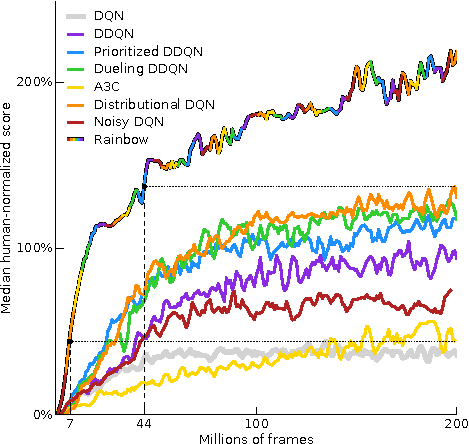
\includegraphics[width=0.5\linewidth]{figures/rainbow-dqn.pdf}
				\caption[Performance of Rainbow \acs{DQN}]{Median performance of Rainbow \acs{DQN} across 57 Atari games; Taken from "Rainbow: Combining Improvements in Deep Reinforcement Learning" (Hessel et al., 2018).}
				\label{fig:rainbowPerformance}
			\end{figure}
		% end
	% end

	\section{Other \acs{DQN}-Based Exploration Techniques}
		In this section we explore some other techniques based on \ac{DQN}, mainly to improve exploration.

		\subsection{Count-Based Exploration}
			Some environment such as jump-n-run games are simply too difficult to be solved. Some reasons for this are sparse rewards (i.e., you only rarely get any reward such as at the end of the episode), complex dynamics, and a high probability of failures (such that it is hard to success by chance). One approach for tackling this problem is to alter the extrinsic (environmental) rewards \(R_\mathrm{ext}(s, a)\) by adding an \emph{intrinsic} rewards \(R_\mathrm{int}(s, a)\):
			\begin{equation}
				R_\mathrm{tot}(s, a) = R_\mathrm{ext}(s, a) + R_\mathrm{int}(s, a).
			\end{equation}
			In order to guide the agent towards exploration, we increase the intrinsic reward in places the agent has visited only a few times,
			\begin{equation}
				R_\mathrm{int}(s, a) = \beta \bigl( N(s) + 0.01 \bigr)^{-1/2},
			\end{equation}
			where \(N(s)\) is the number of times \(s\) was visited and \(\beta\) is a hyper-parameter. We call the idea of exploring where we are uncertain \emph{optimism in the face of uncertainty} and the concrete approach \emph{count-based exploration.} While this approach is straightforward for discrete state-spaces, we cannot just count occurrences in continuous spaces. Instead, we have to define some notion of \emph{similarity} (usually found using unsupervised learning like clustering, \ac{KDE}, auto-encoders, etc.) and count similar states. These counts are then \emph{pseudo-counts.}
		% end

		\subsection{Curiosity-Driven Exploration}
			In \emph{curiosity-driven exploration}, we also add an intrinsic reward \(R_\mathrm{int}(s, a)\), but we use a notion of \emph{curiosity} and want to explore where the knowledge of our model is bad. We hypothesize that states are more interesting if the distance of the predicted next state to the actual next state is large. Hence, we use the intrinsic reward
			\begin{equation}
				R_\mathrm{int}(s, a) = \frac{\eta}{2} \bigl\lVert \vec{\phi}(\tilde{s}') - \vec{\phi}(s') \bigr\lVert_2^2
			\end{equation}
			where \(\tilde{s}'\) is the predicted and \(s'\) is the actual next state and \(\eta\) is a hyper-parameter.
		% end

		\subsection{Ensemble-Driven Exploration}
			Instead of learning a single action-value function, in \emph{ensemble-driven exploration} we train multiple value functions as an ensemble. The ensemble itself is usually implemented by as single \ac{NN} with \(\kappa\) regression heads. During training, each head is trained with different samples where the samples are chosen according to some masking distribution and the value function for acting in the environment is chosen once per trajectory. The corresponding algorithm is called \emph{bootstrapped \ac{DQN}.}
		% end
	% end

	\section{Wrap-Up}
		\begin{itemize}
			\item curse of dimensionality and its effect in \ac{RL}
			\item deep learning in \ac{RL} for handling high-dimensional problems
			\item problems of deep \ac{RL} and some techniques addressing them
			\item the \ac{DQN} algorithm and how to set up experiments with it
			\item enhancing \ac{DQN} by improving function approximation and sample usage
			\item improving key problems of \ac{RL}, e.g., exploration, by combining deep learning techniques and \ac{DQN}
			\item Additional reading material:
				\begin{itemize}
					\item Paper: "Playing Atari with Deep Reinforcement Learning" (Mnih et al., 2013)  % TODO: Read!
					\item Paper: "Deep Reinforcement Learning with Double Q-Learning" (Hasselt et al., 2016)  % TODO: Read!
					\item Paper: "A Distributional Perspective on Reinforcement Learning" (Bellemare et al., 2017)  % TODO: Read!
					\item Paper: "Curiosity-Driven Exploration by Self-Supervised Prediction" (Pathak et al., 2017)  % TODO: Read!
				\end{itemize}
		\end{itemize}
	% end
% end

\chapter{Deep Actor-Critic} % 8.1, 8.6, 8.7, 8.8, 8.9; 8.15
	\label{c:deepAC}

	\todo{Content}

	\section{Surrogate Loss} % 8.10, 8.11, 8.12
		\todo{Content}

		\subsection{Kakade-Langford-Lemma} % 8.13+
			\todo{Content}
		% end

		\subsection{Practical Surrogate Loss} % 8.14
			\todo{Content}
		% end
	% end

	\section{Advantage Actor-Critic (\acs{A2C})} % 8.16, 8.17, 8.18
		\todo{Content}
	% end

	\section{On-Policy Methods} % 8.19
		\todo{Content}

		\subsection{Trust-Region Policy Optimization (\acs{TRPO})} % 8.20, 8.21, 8.28
			\todo{Content}

			\subsubsection{Practical Implementation} % 8.22, 8.23
				\todo{Content}
			% end

			\subsubsection{Conjugate Gradient} % 8.24, 8.25, 8.26, 8.27
				\todo{Content}
			% end
		% end

		\subsection{Proximal Policy Optimization (\acs{PPO})} % 8.29, 8.30
			\todo{Content}
		% end
	% end

	\section{Off-Policy Methods} % 8.31
		\todo{Content}

		\subsection{Deep Deterministic Policy Gradient (\acs{DDPG})} % 8.32, 8.33, 8.34, 8.35
			\todo{Content}
		% end

		\subsection{Twin Delayed DDPG (\acs{TD3})} % 8.36, 8.37
			\todo{Content}
		% end

		\subsection{Soft Actor-Critic (\acs{SAC})} % 8.38, 8.39, 8.40, 8.43, 8.44, 8.45
			\todo{Content}
		% end
	% end

	\section{Wrap-Up} % 8.46, 8.47, 8.48
		\todo{Content}
	% end
% end

\chapter{Frontiers} % 9.1
	\todo{Content}

	\section{Partial Observability} % 9.2, 9.3, 9.4, 9.5, 9.6, 9.7
		\todo{Content}
	% end

	\section{Hierarchical Control} % 9.8, 9.9, 9.10, 9.17
		\todo{Content}

		\subsection{The Options Framework} % 9.11, 9.12, 9.13, 9.14, 9.15, 9.16
			\todo{Content}
		% end
	% end

	\section{Markov Decision Processed Without Reward} % 9.18, 9.19
		\todo{Content}

		\subsection{Intrinsic Motivation} % 9.20, 9.21, 9.22
			\todo{Content}
		% end

		\subsection{Inverse Reinforcement Learning} % 9.23, 9.24, 9.25, 9.26, 9.27
			\todo{Content}
		% end
	% end

	\section{Model-Based Reinforcement Learning} % 9.28, 9.29, 9.30, 9.31, 9.32, 9.33, 9.34
		\todo{Content}
	% end

	\section{Wrap-Up} % 9.35, 9.36
		\todo{Content}
	% end
% end
